\documentclass[10pt]{scrartcl}

% $Id: manual.tex 374 2019-09-14 14:02:58Z jansieber $
%
%\usepackage{CWTWcover}
%\pdfoutput=1
\usepackage[T1]{fontenc}
\usepackage[labelfont={small},textfont={small}]{caption}
\usepackage{subcaption}
\usepackage{tocloft}
% packages from 2.00
\usepackage{amssymb}
\usepackage{graphicx}
\usepackage{amsmath}
%\usepackage{subfigure}
% use other font during editing for better screen readability
\usepackage[scaled=0.9]{helvet}
\usepackage{mathpazo}%[charter]{mathdesign}
% \usepackage[notcite,notref]{showkeys}
% % new packages
% \renewcommand\cftsecfont{\normalfont}
% \renewcommand\cftsecpagefont{\normalfont}
% \renewcommand{\cftsecleader}{\cftdotfill{\cftsecdotsep}}
% \renewcommand\cftsecdotsep{\cftdot}
% \renewcommand\cftsubsecdotsep{\cftdot}
\usepackage{paralist}
\usepackage{typearea}
\usepackage{upquote}
\usepackage[writefile]{listings}
\usepackage[dvipsnames]{xcolor}
\usepackage{microtype}
\usepackage{url}
\usepackage[pdftex]{hyperref}
\usepackage{cleveref}
\definecolor{darkblue}{cmyk}{1,1,0,0}
\definecolor{darkred}{cmyk}{0,1,0,0.7}
\hypersetup{colorlinks, anchorcolor=black,
  citecolor=darkblue, filecolor=darkblue,
  menucolor=darkblue,urlcolor=darkblue,linkcolor=darkblue}

\title{{\DDEBIFCODE\ v. \version{}} Manual --- \\
  Bifurcation analysis
          of delay differential equations} 

% vertical listing of the authors     
\author{J. Sieber, K. Engelborghs, T. Luzyanina, G. Samaey, D. Roose}   

% give the date
\date{\today}

% commands, abbreviations (converted from gdef to newcommand)
\newcommand{\DDEBIFCODE}{\textsc{DDE-BIFTOOL}}
\newcommand{\ddebifweb}{\url{https://sourceforge.net/projects/ddebiftool}}
\newcommand{\ddebifarx}{\url{http://arxiv.org/abs/1406.7144}}
\newcommand{\ddebifwebold}{\url{http://twr.cs.kuleuven.be/research/software/delay/ddebiftool.shtml}}
\newcommand{\version}{3.1}
\newcommand{\file}[1]{\textbf{\texttt{#1}}}
\newcommand{\parm}[1]{\mathsf{#1}}
\newcommand{\define}[1]{\emph{#1}}
\newcommand{\demobase}{\url{../demos/index.html}}
\renewcommand{\i}{\mathrm{i}}
\newcommand{\T}{\mathrm{T}}
\renewcommand{\H}{\mathrm{H}}
\renewcommand{\d}{\mathrm{d}}
\newcommand{\RR}{\mathbb{R}}
\newcommand{\NN}{\mathbb{N}}
\newcommand{\ZZ}{\mathbb{Z}}
\newcommand{\CC}{\mathbb{C}}
%\newcommand{\mod}{\operatorname{mod}}
\renewcommand{\Re}{\operatorname{Re}}
\renewcommand{\Im}{\operatorname{Im}}
\newcommand{\defeq}{:=}
\newcommand\numberthis{\addtocounter{equation}{1}\tag{\theequation}}
\renewcommand{\topfraction}{.85}
\renewcommand{\bottomfraction}{.7}
\renewcommand{\textfraction}{.05}
\renewcommand{\floatpagefraction}{.95}
\renewcommand{\dbltopfraction}{.66}
\renewcommand{\dblfloatpagefraction}{.95}
\setcounter{topnumber}{9}
\setcounter{bottomnumber}{9}
\setcounter{totalnumber}{20}
\setcounter{dbltopnumber}{9}


\newsavebox{\savepar}
\newenvironment{boxit}[1]{\begin{center}\begin{lrbox}{\savepar}
  \begin{minipage}[b]{#1}}{\end{minipage}\end{lrbox}\fbox{\usebox{\savepar}}
  \end{center}}
%% settings and abbreviations for code snippets
\definecolor{var}{rgb}{0,0.28,0.28}
\definecolor{keyword}{rgb}{0,0,1}
\definecolor{comment}{rgb}{0,0.5,0}
\definecolor{string}{rgb}{0.6,0,0.5}
\definecolor{errmsg}{rgb}{1,0,0}
\lstset{language=MATLAB,%
  basicstyle={\ttfamily},%
  commentstyle=\color{comment},%
  stringstyle=\color{string},%
  keywordstyle=\color{keyword},%
  identifierstyle=\color{var},%
  showstringspaces=false,%
  numberbychapter=false,%
  upquote=true,%
  firstnumber=auto,%
  captionpos=b,%
  morekeywords={ones,factorial,inf,why,numel,mod,false,%
    true,warning,continue,@,switch,case,sortrows},%
  deletekeywords={beta,gamma,line,angle,type,plot,mesh}%
}
\newcommand{\mlvar}[1]{\lstinline[keywordstyle=\color{var}]!#1!}
\newcommand{\blist}[1]{\mbox{\lstinline!#1!}}
% set typearea here
\typearea{10}
\begin{document}
\pagenumbering{roman}
\maketitle
%\begin{coverpage}
% \begin{abstract}

% \begin{quotation}             
% {\DDEBIFCODE\ v.~\version} is a collection of MATLAB routines for
% numerical bifurcation analysis of systems of delay differential
% equations with discrete constant and state-dependent delays.
% %
% The package supports continuation and stability analysis of steady
% state solutions and periodic solutions.  Further one can compute and
% continue several local and global bifurcations: fold and Hopf
% bifurcations of steady states; folds, period doublings and torus
% bifurcations of periodic orbits; and
% connecting orbits between equilibria.
% %
% To analyse the stability of steady state solutions, approximations are
% computed to the rightmost, stability-determining roots of the
% characteristic equation which can sub\-sequently be used as starting
% values in a Newton procedure.
% %
% For periodic solutions, approximations to the Floquet multipliers are
% computed.  We describe the structure of the package, its routines, and
% its data and method parameter structures.  We illustrate its use
% through a step-by-step analysis of several demonstrations.
% \end{quotation}
% \end{abstract}

% optionally give keywords and CR (CW) or AMS (TW) classifications

\noindent\textbf{\textsf{Keywords}} nonlinear dynamics, 
delay-differential equations, stability analysis, periodic solutions,
collocation methods, numerical bifurcation analysis, state-dependent
delay.

%\textbf{\textsf{AMS classification}}
% Keywords : keyword1, kw2, kw3.
%\CR XXX, YYY, ZZZ               % CR Subject Classification : XXX, YYY, ZZZ.
%Primary 65J15,            % AMS(MOS) Classification : Primary : XXX, Se-
%Secondary 65P05.          % condary : YYY, ZZZ.

%\end{coverpage}

% \leftmargin    0mm
% \rightmargin -20mm

% \title{{\DDEBIFCODE\ v. \version}: a MATLAB package for bifurcation 
% analysis of delay differential equations}

% \author{K.~Engelborghs, T.~Luzyanina, G.~Samaey, J.~Sieber}

%\maketitle
%
%\begin{abstract}
%DDEBIFTOOL is a collection of Matlab routines for
numerical bifurcation analysis of systems of delay differential
equations with discrete constant and state-dependent delays.

The package supports continuation and stability analysis of steady
state solutions and periodic solutions.  Further one can compute and
continue several local and global bifurcations: fold and Hopf
bifurcations of steady states; folds, period doublings and torus
bifurcations of periodic orbits; and
connecting orbits between equilibria.

To analyse the stability of steady state solutions, approximations are
computed to the rightmost, stability-determining roots of the
characteristic equation which can subsequently be used as starting
values in a Newton procedure.

For periodic solutions, approximations to the Floquet multipliers are
computed.  The manual describes the structure of the package, its routines, and
its data and method parameter structures.

%\end{abstract}
\renewcommand{\contentsname}{}
\tableofcontents
\clearpage
\pagenumbering{arabic}
\section{Citation, license, and obtaining the package}
\label{sec:app:get}
{\DDEBIFCODE} % is freely available for scientific (non-commercial)
% use. It
was started by Koen Engelborghs as part of his PhD at
the Computer Science Department of the K.U.Leuven under supervision
of Prof.\ Dirk Roose.

\paragraph{Citation}
Scientific publications for which the package DDE-BIFTOOL has been
used shall mention usage of the package DDE-BIFTOOL, and shall cite
the following publications to ensure proper attribution and
reproducibility:
\begin{compactitem}\item 
  K. Engelborghs, T. Luzyanina, and D. Roose. Numerical bifurcation
  analysis of delay differential equations using DDE-BIFTOOL, ACM
  Trans. Math. Softw. 28 (1), pp. 1-21, 2002.
\item\textbf{(this manual)} J. Sieber, K. Engelborghs, T. Luzyanina,
  G. Samaey, D. Roose . \DDEBIFCODE\ v. \version{} Manual ---
  Bifurcation analysis
          of delay differential equations, \ddebifarx{}.
\end{compactitem}
The implementation of normal forms for equilibria is based on
\begin{compactitem}
\item M.~M.~Bosschaert, B.~Wage and Y.~Kuznetsov: Description of the
  extension \texttt{ddebiftool\_nmfm}
  \url{http://ddebiftool.sourceforge.net/nmfm_extension_description.pdf}, 2015.
\item B. Wage: Normal form computations for Delay Differential
  Equations in DDE-BIFTOOL. Master Thesis, Utrecht University (NL),
  supervised by Y.A. Kuznetsov (\url{http://dspace.library.uu.nl/handle/1874/296912}, 2014.
\item M. M. Bosschaert, S. G. Janssens, Y. A. Kuznetsov: Switching to
  nonhyperbolic cycles from codimension two bifurcations of equilibria
  of delay differential equations. Preprint \url{https://arxiv.org/abs/1903.08276}, 2017.
\end{compactitem}

All versions of this manual from v.~3.0 onward are available at
\ddebifarx{}.
\paragraph{License}
The following terms cover the use of the software package {\DDEBIFCODE}:
\bigskip\hrule
{\ttfamily
\begin{flushleft} {\parindent0pt
    \parskip5pt \input{../tools/license.txt} }
\end{flushleft}
}
\hrule\bigskip

\paragraph{Download}

Upon acceptance of the above terms, one can obtain the package
{\DDEBIFCODE} (version \version{}) from
\begin{quote}
  \ddebifweb{}.
\end{quote}
Versions up to 3.0 and resources on theoretical background continue to
be available (under a different license) on
\begin{quote}
  \ddebifwebold{}.  
\end{quote}
% The web page
% contains also up-to-date information on newer versions and helpful
% resources.

\section{Version history}
\label{sec:changes}

\subsection{Changes from 3.2a to 3.2b}
\label{sec:v32ato32b}
\begin{itemize}
\item Added ability to perform bifurcation analysis on neutral DDEs
  via delay differential algebraic equations, by permitting a constant
  possibly singular matrix $M$ in front of the left-hand side
  derivative $x'(t)$. A demo \blist{ddae_demo} at
  \url{../demos/ddae_demo/html/ddae_demo.html} on a laser model with
  rotational symmetry is included. The default, when $M$ is not
  provided by the user, is the identity matrix.
\item \textbf{(internal)} The methods for solving nonlinear systems
  and the creation of defining systems have been separated. This
  enables the user to replace \DDEBIFCODE{}'s nonlinear methods with
  other standard methods, such as \blist{fsolve} from Matlab's
  optimization toolbox, or the general continuation package
  \textsc{COCO} \cite{DS13}.  New function:
  \begin{lstlisting}
[f,x0,data]=p_correc_setup(funcs,point,free_par,method,...)
  \end{lstlisting}
  after which one may call, for example, \blist{[x,success]=dde_nsolve(f,x0,method)}
  (the Newton iteration routine coming with \DDEBIFCODE{}) or
  \begin{lstlisting}
    x=fsolve(f,x0,...
      optimoptions('fsolve','SpecifyObjectiveGradient',true))
  \end{lstlisting}
  when using the optimization toolbox routine \blist{fsolve}.
\item A set of demos in folder \url{../demos/coco} and the functions
  in folder \url{../ddebiftool_coco} demonstrate how to create an
  interface to other nonlinear packages by creating an interface for
  \textsc{COCO}. The \textsc{COCO} atlas algorithm has additional
  features such as multi-parameter (e.g. surface) continuation and
  online monitoring of monitoring parameters that are currently not
  implemented in \DDEBIFCODE{}'s native algorithm (\blist{br_contn}).
\item Support for storing collocation polynomials on non-equidistant
  grids on each subinterval, together with pre-defined options of
  storing the polynomials on Chebyshev grids (options
  \blist{'submesh','cheb'} for \blist{SetupPsol}) for periodic
  orbits. This permits collocation polynomials of arbitrarily large
  degree $d$. Note that the computation of error estimates for
  remeshing computes the $d$th derivative, which may become affected
  by numerical overflow for very large degrees.

  The \blist{method.point} field \blist{collocation_parameters} can
  now have one of the names \blist{'legendre'} or \blist{'cheb'} to
  specify in which points on each collocation intervals the DDE is
  enforced.
\item Additional demo \url{../demos/linear_stability} demonstrates
  problems that may occur when computing linear stability of
  equilibria.
\item \textbf{(internal)} The routines for computation of folds of
  periodic orbits have been generalized such that they can be used for
  problems with rotational symmetry.
\item \textbf{(internal, may lead to small changes in behaviour)}
  Utility functions \blist{SetupStst}, \blist{SetupHopf},
  \blist{SetupFold}, \blist{SetupTorusBifurcation},
  \blist{SetupPOfold} etc now perform their initial corrections
  orthogonal to the tangent of the nullspace of the Jacobian in the
  initial guess. Correspondingly, their initial step is along the
  tangent, affecting the meaning of the initial stepsize. This should
  be more robust (permitting starting in folds) but may lead to small
  changes in the computational behaviour (number of steps required
  along branch etc).
\end{itemize}

\subsection{Changes from 3.1.1 to 3.2a}
\label{sec:v311to32a}
\begin{itemize}
\item Added normal form analysis and utility functions for branch
  switching from some steady-state bifurcations of codimension 2 to
  periodic orbit bifurcation of codimension 1 (for state-dependent and
  constant delays). Demos:
  \begin{itemize}
  \item \url{../demos/minimal_demo/html/minimal_demo.html},
  \item \url{../demos/cusp/html/cusp.html}.
  \end{itemize}
(demos \texttt{minimal\_demo}, \texttt{cusp} and tutorials.
\item Added tutorials in folder \texttt{demos} (by M.~M.~Boscchaert).
\item Added ability to automatically generate right-hand side and
  derivatives using symbolic toolbox (folder
  \texttt{ddebiftool\_extra\_nmfm} and demos \texttt{minimal\_demo},
  \texttt{cusp}, \texttt{MackeyGlass}, \texttt{neuron}.
\item Changed default stability computation to Chebyshev-based
  pseudo-spectral method, as in TRACE-DDE \cite{breda09}
  (\blist{dde_stst_eig_cheb}).
\item Added experimental options \blist{'sparse'} for computation of
  periodic orbits and their stability.
\end{itemize}
\subsection{Changes from 3.1 to 3.1.1}
\label{sec:v31to311}
\begin{itemize}
\item Small bug fix: when changing focus on plot window during
  \blist{br_contn}, the online plotting no longer follows focus. This
  keeps the online bifurcation diagram in the same window. An optional
  named argument \blist{'plotaxis'} has been added to \blist{br_contn}
  to explicitly set the plot axes.
\item Added support for rotations (phase oscillators). Periodicity is
  enforced only up to multiples of $2\pi$. Demo
  \url{../demos/phase_oscillator/html/phase_oscillator.html} shows
  how one can track rotations. Demo was contributed by Azamat Yeldesbay.
\item Demos showing detection and computation of Bodganov-Takens
  bifurcation in
  \begin{quote}
    \url{../demos/Holling-Tanner/html/HollingTanner_demo.html}
  \end{quote}
  and cusp in
  \begin{quote}
    \url{../demos/cusp/html/cusp_demo.html}.
  \end{quote}
  Contributed by M.~M.~Boschaert and Y.~Kuznetsov.
\item A description of
  the mathematical formulas behind the normal form computations is now
  in \url{nmfm_extension_description.pdf}, by M.Bossschaert, B.~Wage,
  Y.~Kuznetsov.
\end{itemize}
\subsection{Changes from 3.0 to 3.1}
\label{sec:v3to31}
\paragraph{Change of License and move to Sourceforge}
D. Roose has permitted to change the license to a
Sourceforge-compliant BSD License. Thus, code and newest releases from
version 3.1 onward are now available from \ddebifweb{}. Older versions
will continue to be available from \ddebifwebold{}.
\paragraph{New feature: Normal form computation for bifurcations of
  equilibria}
The new functionality is only applicable for equations with constant
delay. Normal form coefficients can be computed through the extension
\texttt{ddebiftool\_extra\_nmfm}. This extension is included in the
standard \DDEBIFCODE{} archive, but the additional functions are kept
in a separate folder. The following bifurcations are currently
supported.
\begin{itemize}
\item Hopf bifurcation (coefficient $L_1$ determining criticality),
\item generalized Hopf (Bautin) bifurcation (of codimension two,
  typically encountered along Hopf curves)
\item Zero-Hopf interaction (Gavrilov-Guckenheimer bifurcation, of codimension two,
  typically encountered along Hopf curves)
\item Hopf-Hopf interaction (of codimension two, typically encountered
  along Hopf curves) 
\end{itemize}
The extension comes with a demo \texttt{nmfm\_demo}. The demos
\texttt{neuron}, \texttt{minimal\_demo} and \texttt{Mackey-Glass}
illustrate the new functionality, too. Background theory is given in \cite{W14}.
\subsection{Changes from 2.03 to 3.0}
\label{sec:v2to3}

\paragraph{New features}
\begin{itemize}
\item\label{int:pocont} \textbf{\textsf{Continuation of local periodic orbit
    bifurcations}} for systems with constant or state-dependent delay
  is now supported through the extension \texttt{ddebiftool\_extra\_psol}. This
  extension is included in the standard \DDEBIFCODE{} archive, but the
  additional functions are kept in a separate folder.
\item \textbf{\textsf{User-defined functions}} specifying the right-hand side
  and delays (such as \blist{sys_rhs} and \blist{sys_tau}) can have
  arbitrary names.  These user functions (with arbitrary names) get
  collected in a structure \blist{funcs}, which gets then passed on to
  the \DDEBIFCODE{} routines. This interface is similar to other
  functions acting on MATLAB functions such as \blist{fzero} or
  \blist{ode45}. It enables users to add extensions such as
  \texttt{ddebiftool\_extra\_psol} without changing the core routines.
\item \textbf{\textsf{State-dependent delays}} can now have arbitrary levels of
  nesting (for example, periodic orbits of $\dot
  x(t)=\mu-x(t-x(t-x(t-x(t))))$ and their bifurcations can be
  tracked).
\item \textbf{\textsf{Vectorization}}\quad Continuation of periodic orbits
  and their bifurcations benefits (moderately) from
  vectorization of the user-defined functions.
\item \textbf{\textsf{Utilities}}\quad Recurring tasks (such as branching
  off at bifurcations, defining initial pieces of branches, or
  extracting the number of unstable eigenvalues) can now be performed
  more conveniently with some auxiliary functions provided in a
  separate folder \texttt{ddebiftool\_utilities}. See
  \url{../demos/neuron/html/demo1_simple.html} for a demonstration.
\item \textbf{\textsf{Bugs fixed}}\quad Some bugs and problems have been
  fixed in the implementation of the heuristics applied to choose the
  stepsize in the computation of eigenvalues of equilibria
  \cite{VLR08}.
\item \textbf{\textsf{Continuation of relative equilibiria and
      relative periodic orbits}} and their local bifurcations for
  systems with constant delay and rotational symmetry (saddle-node
  bifurcation, Hopf bifurcation, period-doubling, and torus
  bifurcation) is now supported through the extension
  \texttt{ddebiftool\_extra\_rotsym}.
\end{itemize}
Extensions come with demos and separate documentation.

\paragraph{Change of user interface}
Versions from 3.0 onward have a different the user interface for many
\DDEBIFCODE{} functions than versions up to 2.03. They add one
additional input argument \blist{funcs} (this new argument comes
always \emph{first}).  Since \DDEBIFCODE{} v.\,3.0 changed the user
interface, scripts written for \DDEBIFCODE{} v.\,2.0x or earlier will
not work with versions later than 3.0. For this reason version 2.03
will continue to be available. Users of both versions should ensure
that only one version is in the MATLAB path at any time to avoid
naming conflicts.

\section{Capabilities and related reading and
  software}
\label{sec:intro} {\DDEBIFCODE} consists of a set of routines running
in \texttt{MATLAB}\footnote{\url{http://www.mathworks.com}}
\cite{Mat00} or GNU
Octave\footnote{\url{http://www.gnu.org/software/octave}}, both widely
used environments for scientific computing.  The aim of the package is
to provide a tool for numerical bifurcation analysis of steady state
solutions and periodic solutions of differential equations with
constant delays (called DDEs) or state-dependent delays (here called
sd-DDEs). The equations may also be of \emph{neutral} type, when they
are specified i nthe form of delay differential algebraic equations
(here called NDDEs). It also allows users to compute homoclinic and
heteroclinic orbits in DDEs (not NDDEs) with constant delays.

\paragraph{Capabilities}
{\DDEBIFCODE} can perform the following computations:
\begin{compactitem}
\item continuation of steady state solutions (typically in a single
  parameter);
\item approximation of the rightmost, stability-determining roots of
  the characteristic equation which can further be corrected using a
  Newton iteration (for NDDEs computations of roots closest to $0$ is
  recommended);
\item continuation of steady state folds and Hopf bifurcations
  (typically in two system parameters);
\item continuation of periodic orbits using polynomial collocation
  with adaptive mesh selection (starting from a previously computed
  Hopf point or an initial guess of a periodic solution profile);
\item approximation of the largest stability-determining Floquet
  multipliers of periodic orbits (alternatively, the Floquet
  multipliers closest to some complex value $c$);
\item branching onto the secondary branch of periodic solutions at a
  period doubling bifurcation or a branch point;
\item continuation of folds, period doublings and torus bifurcations
  (typically in two system parameters) using the extension
  \texttt{ddebiftool\_extra\_psol};
\item computation of normal form coefficients for Hopf bifurcations
  and codimension-two bifurcations along Hopf bifurcation curves
  (typically in two system parameters) using the extension
  \texttt{ddebiftool\_extra\_nmfm};
\item branching off from codimension-two steady-state bifurcations to
  secondary codimension-one bifurcations using the extension
  \texttt{ddebiftool\_extra\_nmfm} and utility functions from
  \texttt{ddebiftool\_utilities};
\item continuation of connecting orbits (using the appropriate number
  of parameters).  
\end{compactitem}
All computations can be performed for problems with an arbitrary
number of discrete delays. These delays can be either parameters
(DDEs) or functions of the state (sd-DDEs).  The only exception are
computations of connecting orbits, which support only problems with
delays as parameters (and exclude NDDEs and the use of Chebyshev
polynomials) at the moment.

A practical difference to AUTO, MatCont or \textsc{COCO} is that the package
does not detect bifurcations automatically because the computation of
eigenvalues or Floquet multipliers may require more computational
effort than the computation of the equilibria or periodic orbits (for
example, if the system dimension is small but one delay is
large). Instead the evolution of the eigenvalues can be computed along
solution branches in a separate step if required. This allows the user
to detect and identify bifurcations.

% \paragraph{Availability}
% The package is freely available for scientific use.  % A list of the
% % files which constitute {\DDEBIFCODE} is contained in
% % \ref{sec:app:files}.
% A copyright and warranty notice together with
% instructions on obtaining the package can be found in
% Appendix~\ref{sec:app:get}.  Up-to-date information can be found on the web
% page
% \begin{quote}
%   \ddebifweb{}.
% \end{quote}
% Note that the package is typical research software and is provided "as
% is" without warranty of any kind (see \ref{sec:app:get}).

% \DDEBIFCODE{} v. 2.00 is compatible with the previous
% versions. This manual describes both the material of v. 1.00 
% and the extensions of v. 2.00 (support for sd-DDEs and connecting orbits).

\paragraph{About this manual --- related reading}
This manual documents version~\version. Earlier versions of the manual
for earlier versions of \DDEBIFCODE{} continue to be available at the
web addresses
\begin{tabbing}
  versions $\geq3.0$\qquad \= \ddebifarx{}\\
  versions $\leq2.03$ \> \ddebifwebold{}.
\end{tabbing}
For readers who intend to analyse only systems with constant delays,
the parts of the manual related to systems with state-dependent delays
can be skipped (sections \ref{sd_dde}, \ref{sys_def2}).  In the rest
of this manual we assume the reader is familiar with the notion of a
delay differential equation and with the basic concepts of bifurcation
analysis for ordinary differential equations.  The theory on delay
differential equations and a large number of examples are described in
several books. Most notably the early references
\cite{Bell63,Driv77,El's73,Hale77a,Kolm86} and the more recent
references \cite{Azbe91,Kolm92,Hale93,Diek95,Kolm99}.  Several
excellent books contain introductions to dynamical systems and
bifurcation theory of ordinary differential equations, see, e.g.,
\cite{Argy94,Chow82,Guck83,Kuzn04,Seyd94}. For background on numerical
continuation methods one may refer to the textbooks
\cite{DS13,Doed07,G00}.

\paragraph{Tutorial demos}
The tutorial demos \texttt{demo1}, \texttt{minimal\_demo} and
\texttt{sd\_demo}, providing a step-by-step walk-through for the
typical working mode with \DDEBIFCODE{} are included as separate
\texttt{html} files, published directly from the comments in the demo
code. See \demobase{} for links to all demos, many of which are
extensively commented.

For versions prior to 3.0 constructing a branch required creating two
initial guesses and correcting them to obtain the first two points
along the branch. From 3.0 onwards these recurring tasks have been
wrapped in utility functions in folder
\texttt{ddebiftool\_utilities}. These utility functions provide
additional robustness by correcting and predicting along the tangent
and ensuring default initialization of all fields in stuctures. For
these reasons using the utility functions is now the preferred way of
using \DDEBIFCODE{}. Most demos rely on them. Some demos (see
\texttt{demo1}) still demonstrate the use of low-level functions.


\paragraph{Related software}
A large number of packages exist for numerical continuation and
bifurcation analysis of systems of ordinary differential
equations. Currently maintained packages are
\begin{tabbing}
  \texttt{AUTO}\qquad
  \= url: \url{http://sourceforge.net/projects/auto-07p}\qquad\=
  using FORTRAN or C \cite{Doed99,Doed07},\\
  \texttt{MatCont}\>url: \url{http://sourceforge.net/projects/matcont/}\>
  for MATLAB \cite{DGK03,G00}, and\\
  \textsc{COCO}\> url: \url{http://sourceforge.net/projects/cocotools}\> for
  MATLAB \cite{DS13}.\\[1ex]
  For delay differential equations the package\\[0.5ex]
  \texttt{knut}\> url: \url{https://rs1909.github.io/knut/}\> using C++
\end{tabbing}
(formerly \texttt{PDDECONT}) is available as a stand-alone package
(written in C++, but with a user interface requiring no
programming). This package was developed in parallel with
\DDEBIFCODE{} but independently by R.~Szalai \cite{SSH06,RS07}.  For
simulation (time integration) of delay differential equations the
reader is, e.g., referred to the packages ARCHI, DKLAG6, XPPAUT,
DDVERK, RADAR and dde23, see
\cite{Paul95,Thom97,Erme98,Enri97,Sham00,Gugl07}. Julia has a suite of
time integrators able to treat state-dependent and constant delays
\cite{RN17Julia}. Of these, only XPPAUT has a graphical interface (and
allows limited stability analysis of steady state solutions of DDEs
along the lines of \cite{Luzy96}). TRACE-DDE is a MATLAB tool (with
graphical interface) for linear stability analysis of linear
constant-coefficient DDEs
\cite{breda09}.% An up-to-date list of (and links to) available
% software for DDEs can be found on the web page \ddebifweb{}.


% The remainder of this manual is structured as follows.
% In section \ref{code_struct} the structure of {\DDEBIFCODE} is 
% outlined.
% Some necessary notations and properties of delay differential
% equations are briefly described in section \ref{explain_dde}.
% How systems with constant and state-dependent delays can be defined for 
% use inside the package is described in section \ref{sec:system:def}
% by means of two example systems.
% The data structures used to represent points, branches,
% stability information and method parameters are 
% described in section \ref{data_structures}.
% Usage of the code is illustrated  in section \ref{demo}. 
% In section \ref{ride-through}, a step-by-step 
% analysis of the example system with constant delays is described.
% In section \ref{demo2}, specific features in analysis of
% systems with state-dependent delays are shown using
% the example system. Section \ref{demo3} provides a demo
% example for computing connecting orbits.
% Input and output parameter descriptions of routines
% used to compute and manipulate individual points are
% described in section \ref{point_manipulation}.
% Similar descriptions are provided for routines to compute and
% manipulate branches in section \ref{branch_manipulation}.
% More details on the numerical methods and the 
% corresponding method parameters are given in 
% section \ref{numerical_methods}.
% Finally, the report ends with some brief comments on limits to the package
% and future plans in section \ref{limits_sec}.

\begin{figure}[t]
\begin{center}
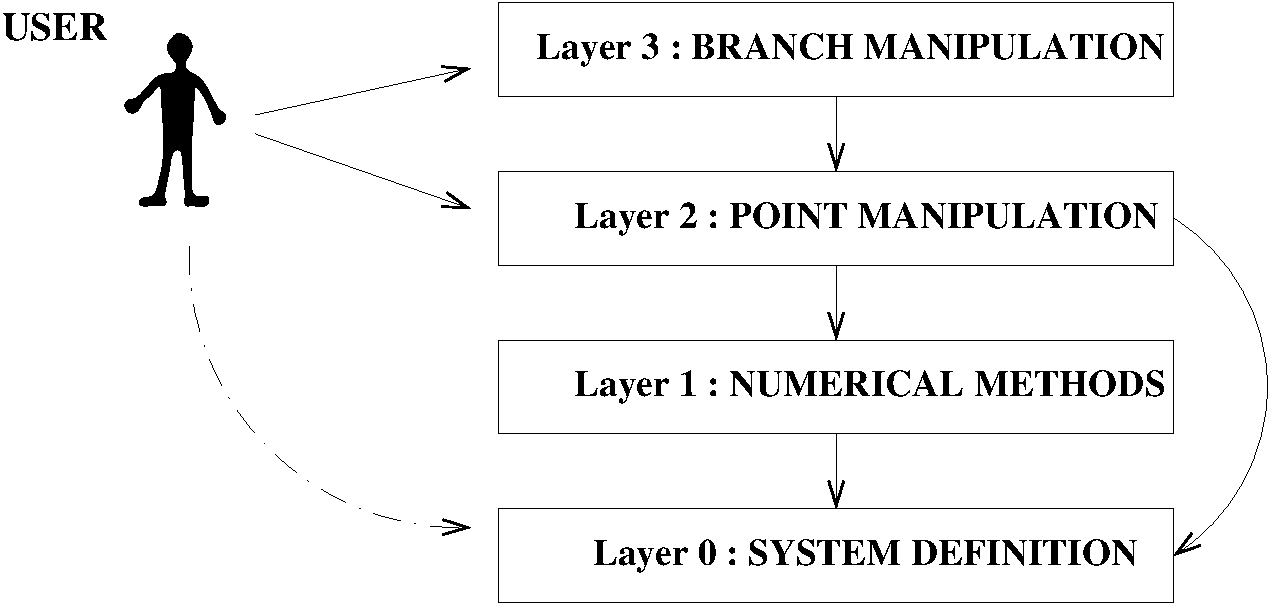
\includegraphics[width=0.8\textwidth]{fig/code_struct}
\end{center}
\caption{\label{struct_pic}
The structure of {\DDEBIFCODE}. Arrows indicate the 
calling ($-$) or writing ($\cdot-$) of routines in a certain layer.} 
\end{figure}

% \bibliographystyle{plain}
% \bibliography{manual}
% \end{document}
\section{Structure of {\DDEBIFCODE}}\label{code_struct}

The structure of the package is depicted in figure \ref{struct_pic}.
It consists of four layers. 

\paragraph{Definition of DDE}
Layer 0 contains the system definition and consists of routines which
allow to evaluate the right hand side $f$ and its derivatives,
state-dependent delays and their derivatives and to set or get the
parameters and the constant delays.  It should be provided by the user
and is explained in more detail in section \ref{sec:system:def}.  All
user-provided functions are collected in a single structure (called
\blist{funcs} in this manual), and are passed on by the user as
arguments to layer-3 or layer-2 functions. It is strongly recommended
that this structure is created using constructors such as
\blist{set_funcs}, \blist{SetupTorusBifurcation}, etc do ensure that
all fields are consistently initialized. \textbf{\emph{Note that this
    is a change in user interface between version 2.03 and
    version~3.0!}}

Layer 1 forms the numerical core of the package and is (normally) not
directly accessed by the user. The defining systems and numerical
methods used are explained briefly in section \ref{numerical_methods},
more details can be found in the papers
\cite{Luzy96,Enge99a,Enge99b,en_d01,engel01,luz01,homoclinic} and in
\cite{Enge00}. Its functionality is hidden by and used through layers
2 and 3. Many of these functions have the prefix \blist{dde_}.

\paragraph{Layer 2 --- Point structures}
Solutions are referred to as \emph{points} in \DDEBIFCODE{}. These are
Matlab \texttt{struct}'s for which \DDEBIFCODE{} has created abstract
functions that can create or manipulate them. A user (or creator of
extensions) can in principle create new \emph{kinds} of points, for
which a specific implementation of point methods and residuals for
layer 1 may have to be then provided.

Layer 2 contains routines to manipulate individual points.  Names of
routines in this layer start with "\file{p\_}".  A point has one of
the following five types.  It can be a steady state point (abbreviated
\blist{'stst'}), steady state Hopf (abbreviated \blist{'hopf'}) or
fold (abbreviated \blist{'fold'}) bifurcation point, a periodic solution point
(abbreviated \blist{'psol'}) or a connecting orbit point (abbreviated
\blist{'hcli'}). Furthermore, a point can contain additional information
concerning its stability.  Routines are provided to compute individual
points, to compute and plot their stability and to convert points from
one type to another.

\paragraph{Layer 3 --- Branch structures}
Layer 3 contains routines to manipulate branches.  Names of routines
in this layer start with "\file{br\_}". A branch is a structure
containing an array of (at least two) points, three sets of method
parameters and specifications concerning the free parameters.  The
\blist{'point'} field of a branch contains an array of points of the
same type ordered along the branch.  The \blist{'method'} field
contains parameters of the computation of individual points, the
continuation strategy and the computation of stability.  The
\blist{'parameter'} field contains specification of the free
parameters (which are allowed to vary along the branch), parameter
bounds and maximal step sizes.  Routines are provided to extend a
given branch (that is, to compute extra points using continuation), to
(re)compute stability along the branch and to visualize the branch
and/or its stability.

Layers 2 and 3 require specific data structures, explained in
section~\ref{data_structures}, to represent points, stability
information, branches, to pass method parameters and to specify
plotting information.  Usage of these layers is
demonstrated %in section~\ref{demo}
through a step-by-step analysis of the demo systems \texttt{neuron},
\texttt{sd\_demo} and \texttt{hom\_demo} (see
\demobase{}).  Descriptions of input/output parameters and
functionality of all routines in layers 2 and 3 are given in
sections~\ref{point_manipulation} respectively
\ref{branch_manipulation}.

\paragraph{Constructor and wrapping utilities}
During construction of branches earlier versions of \DDEBIFCODE{}
required a combination of calls to routines in layer 2 and
3. Constructors in folder \url{../ddebiftool_utilties} automate these
tasks (e.g., \blist{SetupStst}). They also provide additional
automated extraction and creation of stability information
(\blist{GetStability}) plotting (\blist{Plot2dBranch}), branching
(e.g. \blist{ChangeBranchParameters}, \blist{SetupPsol}, 
\blist{BranchFromCodimension2}) and normal form
processing (e.g. \blist{LocateSpecialPoints}).

The distinction between layers (esp. layer 2 and 3) and utilities and
extensions is for historical reasons only. For example, for
computation of linear stability along a branch the utility function
\blist{GetStability} and the layer 3 function \blist{br_stabl} both
call the layer 2 function \blist{p_stabil}, which in turn will call,
for example, the layer 1 function \blist{dde_stst_eig} if the points
in the branch have a suitable \blist{'kind'} field. The utility
function \blist{GetStability} has additional features such as the
counting of unstable eigenvalues depending on \blist{'kind'} field and
the rules provided in \blist{pointtype_list()}.


\section{Delay differential equations}\label{explain_dde}
\label{sec:ddes}
This section introduces the mathematical notation that we refer to in
this manual to describe the problems solved by \DDEBIFCODE{}.
\subsection{Equations with constant delays}\label{dde}

Consider the system of delay differential equations with constant
delays (DDEs),
\begin{equation}\label{the_dde_type}
M\frac{\d}{\d t}{x(t)}=f(x(t),x(t-\tau_1),\ldots,x(t-\tau_m),\eta),
\end{equation}
where $M$ is a constant $n\times n$ matrix, $x(t)\in\RR^n$,
$f:\RR^{n(m+1)}\times\RR^p \rightarrow\RR^n$ is a nonlinear smooth
function depending on a number of parameters $\eta\in\RR^p$, and
delays $\tau_i>0$, $i=1,\ldots,m$.  Call $\tau$ the maximal delay,
\[
\tau=\max_{i=1,\ldots,m}\tau_i.
\]
The linearization of (\ref{the_dde_type}) around a solution $x^*(t)$ 
is the \define{variational equation}, given by,
\begin{equation}\label{the_var_equa}
M\frac{\d}{\d t}{y(t)}=A_0(t)y(t)+\sum_{i=1}^m A_i(t)y(t-\tau_i),
\end{equation}
where, using $f\equiv f(x^0,x^1,\ldots,x^m,\eta)$,  
\begin{equation}\label{A_def}
A_i(t)=\frac{\partial f}{\partial x^i}(x^*(t),x^*(t-\tau_1),\ldots,x^*(t-\tau_m),\eta), 
\ i=0,\ldots,m. 
\end{equation}
For regular $M$ \cref{the_dde_type} is a classical DDE. For singular
$M$, equations of type \eqref{the_dde_type} can create a variety of
different types of equation, including differential algebraic
equations, backward-forward equations and neutral DDEs (NDDEs). \DDEBIFCODE{}
is tested only for neutral DDEs. Consider a NDDE of the form analysed by Hale\& Verduyn-Lunel \cite{Hale93}
\begin{equation}
  \label{eq:nddepure}
  \frac{\d}{\d t}\left[z(t)+f_l(z(t),z(t-\tau_1),\ldots,z(t-\tau_m),\eta)\right]
  =f_r(z(t),z(t-\tau_1),\ldots,z(t-\tau_m),\eta)
\end{equation}
with $n_z$-dimensional $z$.
Equation~\eqref{eq:nddepure} can then be put into the form \eqref{the_dde_type} of dimension $n=2n_z$ with
\begin{align*}
  M&=
  \begin{bmatrix}
    I&0 \\ 0&0 
  \end{bmatrix}\mbox{,}&
  x(t)&=
  \begin{bmatrix}
    y(t)\\ z(t)
  \end{bmatrix}\mbox{,}&
  f\left(
    \begin{bmatrix}
      y_0\\ z_0
    \end{bmatrix}
,     \begin{bmatrix}
      y_1\\ z_1
    \end{bmatrix}
    ,\ldots
        \begin{bmatrix}
      y_m\\ z_m
    \end{bmatrix},\eta\right)&=
  \begin{bmatrix}
    f_r(z_0,z_1,\ldots z_m,\eta)\\
    z_0+f_l(z_0,z_1,\ldots z_m,\eta)-y_0
  \end{bmatrix}
\end{align*}
and the same delays $\tau_1$,\ldots,$\tau_m$. Demos exist only for this type of equation.

\subsubsection{Steady states}
\label{sec:dde:stst}
If $x^*(t)$ corresponds to a steady state solution,
\[
x^*(t)\equiv x^*\in\RR^n,\mathrm{\ with\ }f(x^*,x^*,\ldots,x^*,\eta)=0,
\]
then the matrices 
$A_i(t)$ are constant, $A_i(t)\equiv A_i$, and the corresponding 
variational equation (\ref{the_var_equa})
leads to a \define{characteristic equation}. Define the $n\times n$-dimensional
matrix $\Delta$ as
\begin{equation}
  \Delta(\lambda)=\lambda M - A_0 - \sum_{i=1}^m A_i e^{-\lambda\tau_i}.
\label{eq:deltadef}
\end{equation}
Then the characteristic equation reads,
\begin{equation}\label{the_char_eq}
\det(\Delta(\lambda))=0.
\end{equation}
Equation (\ref{the_char_eq}) has an infinite number of roots
$\lambda\in\CC$ which determine the stability of the steady state
solution $x^*$.  The steady state solution is (asymptotically) stable
provided all roots of the characteristic equation (\ref{the_char_eq})
have negative real part; it is unstable if there exists a root with
positive real part. For regular $M$ (classical DDEs) it is known that
the number of roots in any right half plane $\Re(\lambda)>\gamma$,
$\gamma\in\RR$ is finite, hence, the stability is always determined by
a finite number of roots.

Bifurcations occur whenever roots move through the imaginary
axis as one or more parameters are changed.
Generically a fold bifurcation (or turning point) occurs when
the root is real (that is, equal to zero) and a 
Hopf bifurcation occurs when a pair of complex conjugate roots crosses the imaginary axis.

\subsubsection{Periodic orbits}
\label{sec:dde:psol}
A periodic solution $x^*(t)$ is a solution which repeats itself after
a finite time, that is,
\[ 
x^*(t+T)=x^*(t),\mathrm{\ for\ all\ }t. 
\]
Here $T>0$ is the period.  The stability around the periodic solution
is determined by the time integration operator $S(T,0)$ which
integrates the variational equation (\ref{the_var_equa}) around
$x^*(t)$ from time $t=0$ over the period.  This operator is called the
\define{monodromy operator} and its (infinite number of) eigenvalues,
which are independent of the starting moment $t=0$, are called the
\define{Floquet multipliers}.  Furthermore, for classical DDEs ($M=I$) the operator
$S(T,0)^k=S(kT,0)$ is compact for $k>\tau/T$. Thus, there are at most finitely
many Floquet multipliers outside of any ball around the origin of the
complex plane.

For autonomous systems there is always a \define{trivial} Floquet
multiplier at unity, corresponding to a perturbation along the time
derivative of the periodic solution. The periodic solution is
exponentially stable provided all multipliers (except the trivial one)
have modulus smaller than unity, it is exponentially unstable if there
exists a multiplier with modulus larger than unity. \emph{Local
  bifurcations} are characterized by additional Floquet multipliers on
the unit circle:
\begin{compactitem}
\item Fold of periodic orbits (\blist{POfold}): double Floquet multiplier at $1$;
\item Period doubling (\blist{PeriodDoubling}): Floquet multiplier at $-1$;
\item Torus vbifurcation (\blist{TorusBifurcation}): complex pair of
  Floquet multipliers $\exp(\pm\i\pi\omega)$ with $\omega\in(0,1/2)$.
\end{compactitem}


%G's addition
\subsubsection{Connecting orbits}
\label{sec:dde:hcli}
We call a solution $x^*(t)$ of \cref{the_dde_type} at $\eta=\eta^*$ a 
\textit{connecting orbit} if the limits 
\begin{equation}
\lim_{t\to -\infty} x^*(t)=x^{-}, \qquad \lim_{t\to +\infty} x^*(t)=x^{+},
\end{equation}
exist.  For continuous $f$, $x^-$ and $x^+$ 
are steady state solutions. 
If $x^-=x^+$, the orbit is called homoclinic, otherwise it is heteroclinic. 
%end of G's addition

\subsection{Equations with state-dependent delays}\label{sd_dde}

Consider the system of delay differential equations with
state-dependent delays (sd-DDEs),
\begin{equation}\label{the_dde_type2}
\left\{
\begin{aligned}
M\frac{\d}{\d t}{x(t)}&=f(x_0,x_1,\ldots,x_m,\eta)\mbox{,\quad with}\\
x_j&=x(t-\tau_j(x_0,\ldots,x_{j-1},\eta)\quad\mbox{($\tau_0=0$, $j=1,\ldots,m$)}\mbox{,}
\end{aligned}
\right.
\end{equation}
where $x(t)\in\RR^n$, and
\begin{align*}
 f:&\RR^{n(m+1)}\times\RR^p \to\RR^n\\
 \tau_j:&\RR^{n\,j}\times\RR^p\to[0,\infty)
\end{align*}
are smooth functions depending of their arguments. The right-hand side
$f$ depends on $m+1$ states $x_j=x(t-\tau_j)\in\RR^n$ ($j=0,\ldots,m$)
and $p$ parameters $\eta\in\RR^p$. The $j$th delay function $\tau_j$
depends on all previously defined $j-1$ states $x(t-\tau_i)\in\RR^n$
($i=0,\ldots,j-1$) and $p$ parameters $\eta\in\RR^p$. This
definition permits the user to formulate sd-DDEs with arbitrary levels
of nesting in their function arguments.

The linearization around a solution $(x^*(t),\eta^*)$ of
\eqref{the_dde_type2} (the \define{variational equation}) with respect
to $x$ is given by (see \cite{HKWW06}, we are using the notation
$x^*_0=x^*(t)$, $\tau_j^*(t)=\tau_j(x^*_0,\ldots,x^*_{j-1},\eta^*)$ and
$x^*_j=x^*(t-\tau^*_j(t))$ for $j\geq1$)
\begin{equation}\label{the_var_equa2}
\begin{aligned}
M\frac{\d}{\d t}{y(t)}&=\sum_{j=0}^mA_j(t)Y_k \\
Y_0&=y(t)\\
Y_j&=y(t-\tau^*_j(t))-(x^*)'(t-\tau_j(t))\sum_{k=0}^{j-1}B_{k,j}(t)Y_k\mbox{,\quad($j=1\ldots m$)}
\end{aligned}
\end{equation}
where $(x^*)^{'}(t)={\d}x^*(t)/{\d}t$, and
\begin{equation}\label{A_def2}
\begin{aligned}
  A_j(t)&=\frac{\partial f}{\partial x^j}(x^*_0,x^*_1,\ldots,x^*_m,\eta)\in\RR^{n\times n}
  \mbox{,\quad ($j=0,\ldots,m$),}\\
  B_{j,k}(t)&=\frac{\partial \tau_j}{\partial x^k}(x^*_0,x^*_1,\ldots,x^*_{j-1},\eta^*)\in\RR^{1\times n}\mbox{,\quad ($k=0,\ldots,j-1$, $j=1,\ldots,m$).} 
\end{aligned}
\end{equation}

If $(x^*(t))$ corresponds to a steady state
solution, then $x^*(t)=x^*_0=\ldots=x^*_m\equiv x^*\in\RR^n$, and
$\tau^*_j(t)\equiv \tau_j(x^*,\ldots,x^*,\eta^*)$ for all $j\geq1$, with
\[
f(x^*,x^*,\ldots,x^*,\eta^*)=0\mbox{.}
\]
Then the matrices $A_i(t)$ are constant, $A_i(t)\equiv A_i$, and the
vectors $B_{i,j}(t)$ consist of zero elements only.  In this case, the
corresponding variational equation \eqref{the_var_equa2} is a constant
delay differential equation and it leads to the characteristic
equation (\ref{the_char_eq}), i.e.~a characteristic equation with
constant delays. Hence the stability analysis of a steady state
solution of \eqref{the_dde_type2} is identical to the stability analysis
of \eqref{the_dde_type}.

Note that the right-hand side $f$, when considered as a functional
mapping a history segment into $\RR^n$ is not locally Lipschitz
continuous. This creates technical difficulties when considering a
sd-DDE of type \eqref{the_dde_type2} as an infinite-dimensional
system, because the solution does not depend smoothly on the
initial condition (see Hartung \emph{et al. }\cite{HKWW06} for a
detailed review). However, periodic boundary-value problems for
\eqref{the_dde_type2} can be reduced to finite-dimensional systems of
algebraic equations that are as smooth as the coefficient functions
$f$ and $\tau_j$ \cite{S12}. This implies that all periodic orbits and
their bifurcations and stability as computed by \DDEBIFCODE{} behave as
expected. In particular, branching off at Hopf bifurcations and period
doubling works in the same way as for constant delays (the proof for the Hopf
bifurcation in sd-DDEs is also given in \cite{S12}).

% Note that the Hopf bifurcation theorem has not been proven yet for
% sd-DDEs. However 
% the theorems on existence of periodic solutions for sd-DDEs suggest
% that a Hopf bifurcation theorem holds for these  
% equations.
% In the following we will refer to the situation when 
% the characteristic equation has a pair of pure imaginary roots of 
% multiplicity 1 as a {\normalfont\itshape Hopf-like} bifurcation.

% The stability theory of periodic solutions of sd-DDEs 
% has not yet been fully developed in the mathematical literature. 
% Equation~(\ref{the_var_equa2}) is a 
% linear equation with {\normalfont\itshape time-dependent} (no longer state-dependent)
% delays.
% If the coefficients in the linear equation are smooth and periodic (with
% period $T$) and the delay functions are 
% smooth, then this equation belongs to the class of linear
% periodic equations studied in \cite{Hale77a}.
% For these equations, the solution operator over the
% period $T$ is compact.
Moreover, Mallet-Paret and Nussbaum \cite{MN11} proved that the
stability of the linear variational equation \eqref{the_var_equa2}
indeed reflects the {\normalfont\itshape local stability} of the solution
$(x^*(t))$ of \cref{the_dde_type2}. 
For details on the relevant theory and numerical bifurcation analysis
of differential equations with state-dependent delay see
\cite{luz01,HKWW06,S17} and the references therein.

\section{System definition}\label{sec:system:def}

\subsection{Change from \DDEBIFCODE{} v.~3.1 to v.~3.2: symbolic generation}
\label{sec:symbolic}
The folder \url{../ddebiftool_extra_symbolic} contains routines that
enable the user to create right-hand sides, delays (if
state-dependent) and their derivatives through automatic code
generation. The routines rely on either the symbolic toolbox of Matlab
or the package \texttt{symbolic} of Octave (which relies on the
\texttt{sympy} python library). In particular, right-hand sides and
derivatives generated with the symbolic toolbox do not require the
symbolic toolbox to be used in computations. Right-hand sides and
derivatives generated with Octave can be used in Matlab (and vice
versa).

Previous versions had external Mathematica scripts such as
\url{../external_tools/genr_sys.mth}, provided by D. Pieroux (still available).

For manually implemented derivatives, the user may also provide
directional derivatives instead of the more complex Jacobians.
\subsection{Change from \DDEBIFCODE{} v.~2.03 to
  v.~3.0} Note that from \DDEBIFCODE{} v.~3.0 all
user-provided functions can be arbitrary function handles, collected
into a structure using the function \blist{set_funcs}, explained in
section~\ref{sec:funcs}. The only typical mandatory functions for the
user to provide are the right-hand side (\blist{'sys_rhs'}) and the
function returning the delay indices (\blist{'sys_tau'}). The names of
the user functions can be arbitrary, and user functions can be
anonymous. This is a change from versions $<3.0$. See the tutorials
in \demobase{} for examples of usage, and the function description in
section~\ref{sec:funcs} for details.

The new version also supports \textbf{\emph{vectorized}} right-hand
sides and delays, leadingto speed-up in computations involving periodic orbits.
\subsection{Equations with constant delays}\label{sys_def1}

As an illustrative example we will use the following system of delay 
differential
equations, taken from \cite{Shay99},
\begin{equation}\label{example_sys}
\left\{
\begin{array}{l}
\dot{x_1}(t)=-\kappa x_1(t)+\beta \tanh(x_1(t-\tau_s))+a_{12}\tanh(x_2(t-\tau_2)) \\
\dot{x_2}(t)=-\kappa x_2(t)+\beta \tanh(x_2(t-\tau_s))+a_{21}\tanh(x_1(t-\tau_1)) .
\end{array}
\right.
\end{equation}
This system models two coupled neurons with time delayed connections.
It has two components ($x_1$ and $x_2$), three delays ($\tau_1$,
$\tau_2$ and $\tau_s$), and four parameters ($\kappa$, $\beta$,
$a_{12}$ and $a_{21}$).  The demo \texttt{neuron} (see
\demobase{}) walks through the
bifurcation analysis of system \eqref{example_sys} step by step to
demonstrate the working pattern for \DDEBIFCODE.

To define a system, the user should provide the following MATLAB
functions, given in the following paragraphs for system \eqref{example_sys}.

\subsubsection{Right-hand side --- \texorpdfstring{\blist{sys_rhs}}{sys\_rhs}}\label{sec:constrhs} 
The right-hand side is a function of two arguments. For our example
\eqref{example_sys}, this would have the form (giving the right-hand
side the name \blist{neuron_sys_rhs}) given in \Cref{neuron_sys_rhs}.
\begin{lstlisting}[float,frame=lines,label=neuron_sys_rhs,caption={Definition for right-hand side of \eqref{example_sys} as a variable. See \Cref{neuron_sys_rhs_vec} for the vectorized version.}]
neuron_sys_rhs=@(xx,par)[...
  -par(1)*xx(1,1)+par(2)*tanh(xx(1,4))+par(3)*tanh(xx(2,3));...
  -par(1)*xx(2,1)+par(2)*tanh(xx(2,4))+par(4)*tanh(xx(1,2))];  
%par=[\kappa,\beta, a_{12}, a_{21},\tau_1,\tau_2, \tau_s]
\end{lstlisting}
Meaning of the arguments of the right-hand side function:
\begin{itemize}
\item $\blist{xx}\in\RR^{n\times (m+1)}$ contains the state
variable(s) at the present and in the past,
\item $\blist{par}\in\RR^{1\times
  p}$ contains the parameters, $\blist{par}=\eta$.
\end{itemize}
The delays $\tau_i$ ($i=1\ldots,m$) are considered to be part of the
parameters ($\tau_i=\eta_{j(i)}$, $i=1,\ldots,m$).  This is natural
since the stability of steady solutions and the position and stability
of periodic solutions depend on the values of the delays.  Furthermore
delays can occur both as a `physical' parameter and as delay, as in
$\dot{x}=\tau x(t-\tau)$.  From these inputs the right hand side $f$
is evaluated at time $t$. Notice that the parameters have a specific
order in $\parm{par}$ indicated in the comment line.

\paragraph{Vectorization}
An alternative (vectorized) form would be as given in
\Cref{neuron_sys_rhs_vec}.
\begin{lstlisting}[float,frame=lines,label=neuron_sys_rhs_vec,caption={Alternative definition of the right-hand side of \eqref{example_sys}, vectorized for speed-up of periodic orbit computations.}]
  neuron_sys_rhs=@(xx,p)[...
  -p(1)*xx(1,1,:)+p(2)*tanh(xx(1,4,:))+p(3)*tanh(xx(2,3,:));....
  -p(1)*xx(2,1,:)+p(2)*tanh(xx(2,4,:))+p(4)*tanh(xx(1,2,:))];
\end{lstlisting}
Note the additional colon in argument \blist{xx} and compare to
Listing~\ref{neuron_sys_rhs}. The form shown in
Listing~\ref{neuron_sys_rhs_vec} can be called in many points along a
mesh simultaneously, speeding up the computations during analysis of
periodic orbits.

\subsubsection{Delays --- \texorpdfstring{\blist{sys_tau}}{sys\_tau}} \label{sec:consttau}
For constant delays another function is required which returns the
\emph{position} of the delays in the parameter list. For our example,
this is
\begin{lstlisting}
  neuron_tau=@()[5 6 7];
\end{lstlisting}
This function has no arguments for constant delays, and returns a row
vector of indices into the parameter vector.

\subsubsection{Derivatives or Jacobians of right-hand side ---
  \texorpdfstring{\blist{sys_deri}}{sys\_deri} (optional, but
  recommended)}\label{sec:constjac}
\begin{quote}
  \textbf{Note}: See  \blist{sys_dirderi} in
  \cref{sec:dirderi} for alternatively providing directional derivatives.
\end{quote}
Several derivatives of the right hand side function $f$ need to be
evaluated during bifurcation analysis. By default, \DDEBIFCODE{} uses
a finite-difference approximation, implemented in
\blist{dde_dirderiv}, combined with \blist{dde_gen_deriv}. For
speed-up or in case of convergence difficulties the user may provide
the Jacobians of the right-hand side analytically as a separate
function. Its header is of the format
\begin{lstlisting}
  function J=sys_deri(xx,par,nx,np,v)
\end{lstlisting}
Arguments:
\begin{itemize}
\item $\blist{xx}\in\RR^{n\times (m+1)}$ contains the state
variable(s) at the present and in the past (as for the right-hand side);
\item $\blist{par}\in\RR^{1\times
  p}$ contains the parameters, $\blist{par}=\eta$  (as for the right-hand side);
\item \blist{nx} (empty, one integer or two integers) index (indices) of
  \blist{xx} with respect to which the right-hand side is to be
  differentiated
\item \blist{np} (empty or integer) whether right-hand side is to be
  differentiated with respect to parameters
\item \blist{v} (empty or $\CC^n$) for mixed derivatives with respect
  to \blist{xx}, only the product of the mixed derivative with
  \blist{v} is needed.
\end{itemize}
% and should be supplied via a routine \file{sys\_deri.m}.
% The function \file{sys\_deri} has as input variables $\parm{xx}$ and
% $\parm{par}$ (with ordering of state variables and parameters as
% before), $\parm{nx}$, $\parm{np}$ and $\parm{v}$. Here,
% $v\in\CC^{n\times 1}$ or empty. 
The result \blist{J} is a matrix of
partial derivatives of $f$ which depends on the type of derivative
requested via \blist{nx} and \blist{np} multiplied with \blist{v} (when
nonempty), see table \ref{deri_requested}.
\begin{table}[htbp]
\begin{center}
\begin{tabular}{ccc@{\hspace*{5em}}l}
\noalign{\medskip}\hline\noalign{\smallskip}\blist{length(nx)} & \blist{length(np)}  & \blist{v} & \blist{J} 
\\\noalign{\smallskip}\hline\noalign{\medskip}
1         & 0         & empty      & 
$\frac{\textstyle\partial f}{\textstyle\partial x^{\blist{nx(1)}}}
=A_{\blist{nx(1)}}\in\RR^{n\times n}$ \\[3ex]
0         & 1         & empty      & 
$\frac{\textstyle\partial f}{\textstyle\partial \eta_{\blist{np(1)}}}
\in\RR^{n\times 1}$ \\[3ex]
1         & 1         & empty      & 
$\frac{\textstyle\partial^2 f}{\textstyle\partial x^{\blist{nx(1)}}\partial \eta_{\blist{np(1)}}}
\in\RR^{n\times n}$ \\
2         & 0         & $\in\CC^{n\times1}$ & 
$\frac{\textstyle\partial}{\textstyle\partial x^{\blist{nx(2)}}}
\left(A_{\blist{nx(1)}}v\right)
\in\CC^{n\times n}$\\\noalign{\medskip}\hline
\end{tabular}
\caption{\label{deri_requested}
Results of the function \file{sys\_deri} depending on its
input parameters \blist{nx}, \blist{np} and \blist{v}
using $f\equiv f(x^0,x^1,\ldots,x^m,\eta)$.}
\end{center}
\end{table}

\blist{J} is defined as follows. Initialize \blist{J} with $f$. If
\blist{nx} is nonempty take the derivative of \blist{J} with respect
to those arguments listed in \blist{nx}'s entries. Each entry of
\blist{nx} is a number between $0$ and $m$ based on $f\equiv
f(x^0,x^1,\ldots,x^m,\eta)$.  E.g., if \blist{nx} has only one element
take the derivative with respect to $x^{\blist{nx(1)}}$.  If it has
two elements, take, of the result, the derivative with respect to
$x^{\blist{nx(2)}}$ and so on.  Similarly, if \blist{np} is nonempty
take, of the resulting \blist{J}, the derivative with respect to
$\eta_{\blist{np(i)}}$ where $i$ ranges over all the elements of
\blist{np}, $1\leq i \leq p$.  Finally, if $v$ is not an empty vector
multiply the result with $v$.  The latter is used to prevent \blist{J}
from being a tensor if two derivatives with respect to state variables
are taken (when \blist{nx} contains two elements).  Not all possible
combinations of these derivatives have to be provided.  In the current
version, \blist{nx} has at most two elements and \blist{np} at most
one.  The possibilities are further restricted as listed in table
\ref{deri_requested}.

In the last row of table \ref{deri_requested} the elements of \blist{J}
are given by,
\[
\blist{J}_{i,j}=\left[\frac{\partial}{\partial x^{\blist{nx(2)}}}
A_{\blist{nx(1)}}v\right]_{i,j}
=\frac{\partial}{\partial x_j^{\blist{nx(2)}}}
\left(\sum_{k=1}^n\frac{\partial f_i}{\partial x_k^{\parm{nx(1)}}} v_k
\right),
\]
with $A_l$ as defined in \eqref{A_def}.


The resulting routine is quite long, even for the small system
\eqref{example_sys}; see Listing~\ref{neuron:sys:deri} in
Appendix~\ref{sec:sys:deri} for a printout of the function body.  Furthermore,
implementing so many derivatives is an activity prone to a number of
typing mistakes. Hence a default routine \blist{df\_deriv} is
available which implements finite difference formulas to approximate
the requested derivatives (using several calls to the right-hand
side. It is, however, recommended to provide at least the first order
derivatives with respect to the state variables using analytical
formulas. These derivatives occur in the determining systems for fold
and Hopf bifurcations
%G.'s add
and for connecting orbits,  
%end of G.'s add
and in the computation of characteristic roots and Floquet multipliers.
All other derivatives are only necessary in the 
Jacobians of the respective Newton procedures and thus
influence only the convergence speed. 

\subsection{Directional derivatives}
\label{sec:dirderi}
\begin{lstlisting}[float,floatplacement=t,frame=lines,label=neuron_sys_dirderi,caption={First two directional derivatives of right-hand side of \cref{example_sys} (not vectorized, see \url{../demos/neuron/html/demo1_funcs.html} and note that
 provision of this pair of functions is less complex than the routine
 for \blist{neuron_sys_deri} in \Cref{neuron:sys:deri}).}]
dtanh=@(x)(1-tanh(x)^2);
ddtanh=@(x)(tanh(x)^2-1)*2*tanh(x);
neuron_sys_dirderi{1}=@(x,p,dx,dp)[...
 -dp(1)*x(1,1)-p(1)*dx(1,1)+...
  dp(2)*tanh(x(1,4))+p(2)*dtanh(x(1,4))*dx(1,4)+...
  dp(3)*tanh(x(2,3))+p(3)*dtanh(x(2,3))*dx(2,3);...
 -dp(1)*x(2,1)-p(1)*dx(2,1)+...
  dp(2)*tanh(x(2,4))+p(2)*dtanh(x(2,4))*dx(2,4)+...
  dp(4)*tanh(x(1,2))+p(4)*dtanh(x(1,2))*dx(1,2)];
neuron_sys_dirderi{2}=@(x,p,dx,dp)[...
 -2*dp(1)*dx(1,1)+...
  2*dp(2)*dtanh(x(1,4))*dx(1,4)+p(2)*ddtanh(x(1,4))*dx(1,4)^2+...
  2*dp(3)*dtanh(x(2,3))*dx(2,3)+p(3)*ddtanh(x(2,3))*dx(2,3)^2; ...
 -2*dp(1)*dx(2,1)+...
  2*dp(2)*dtanh(x(2,4))*dx(2,4)+p(2)*ddtanh(x(2,4))*dx(2,4)^2+...
  2*dp(4)*dtanh(x(1,2))*dx(1,2)+p(4)*ddtanh(x(1,2))*dx(1,2)^2];
 \end{lstlisting}
As an alternative to the function \blist{sys_deri} the user may
provide directional derivatives. The $k$th directional derivative of
the right-hand side $f(x_0,\ldots,x_m,\eta)$,
\begin{displaymath}
  \d^kf(x_0,\ldots,x_m,\eta)[\tilde{x}_0,\ldots,\tilde{x}_m,\tilde{\eta}]^k:=
  \frac{\d^k}{\d h^k}f(x_0+h\tilde{x}_0,\ldots,x_m+h\tilde{x}_m,\eta+h\tilde{\eta})\vert_{h=0}\mbox{,}
\end{displaymath}
 has to have the form
\begin{lstlisting}
  function J=sys_dirderi(xx,par,dxx,dpar)
\end{lstlisting}
Arguments:
\begin{itemize}
\item $\blist{xx}\in\RR^{n\times (m+1)}$ contains the state
  variable(s), $\blist{xx(:,j)}=x_{j-1}$, $x_0,\ldots,x_m$, at the present and in the past (as
  for the right-hand side),;
\item $\blist{par}\in\RR^{1\times
  p}$ contains the parameters, $\blist{par}=\eta$  (as for the right-hand side);
\item \blist{dxx}$\in\RR^{n\times(m+1)}$ contains the deviations that is applied to
  \blist{xx}: \blist{dxx(:,j)}$=\tilde{x}_{j-1}$ for
    $j=1\ldots,m+1$(empty, one integer or two integers) index
    (indices) of \blist{xx} with respect to which the right-hand side
    is to be differentiated
\item \blist{dpar}$\in\RR^{1\times
  p}$ contains the deviations to the parameters, $\blist{dpar}=\tilde{\eta}$.
\end{itemize}
The user passes on the set of all directional deriviatives in a
$1\times\blist{maxorder}$ cell array to \blist{set_funcs} (see
\cref{sec:funcs}). For standard bifurcation analysis derivatives up to
order $2$ are used. For normal form analysis derivatives up to order
$5$ are used. Any derivatives that are not provided by either
\blist{sys_deri} or \blist{sys_dirderi} will be approximated by finite
differences. For the example \eqref{example_sys}, the first two
directional derivatives can be implemented as given in
\Cref{neuron_sys_dirderi}.  Directional derivatives are easier to
provide in vectorized form.

\subsection{Equations with state-dependent
  delays}\label{sys_def2}
\DDEBIFCODE{} also permits the delays to depend on parameters and the
state. If at least one delay is state-dependent then the format and
semantics of the function specifying the delays, \blist{sys_tau}, is
different from the format used for constant delays in
section~\ref{sec:consttau} (it now provides the \emph{values} of the
delays).  Note that for a system with only constant delays we
recommend the use of the system definitions as described in
section~\ref{sys_def1} to reduce the computational effort.

As an illustrative example we will use the following system of delay 
differential equations,
\begin{equation}\label{example_sys2}
  \begin{split}
    \frac{\d}{\d t}x_1(t)&=\frac{1}{p_1+x_2(t)}\left(1-p_2x_1(t)x_1(t-\tau_3)
      x_3(t-\tau_3)+p_3x_1(t-\tau_1)x_2(t-\tau_2)\right),\\
    \frac{\d}{\d t}x_2(t)&=\frac{p_4 x_1(t)}{p_1+x_2(t)}+
    p_5\tanh(x_2(t-\tau_5))-1,\\
    \frac{\d}{\d t}x_3(t)&=p_6(x_2(t)-x_3(t))-p_7(x_1(t-\tau_6)-x_2(t-\tau_4))e^{-p_8 \tau_5},\\
    \frac{\d}{\d t}x_4(t)&=x_1(t-\tau_4)e^{-p_1 \tau_5} -0.1,\\
    \frac{\d}{\d t}x_5(t)&=3(x_1(t-\tau_2)-x_5(t))-p_9,
  \end{split}
\end{equation}
where
\begin{align*}
\tau_1, \tau_2 &\mbox{ are constant delays},\\
\tau_3&=2+p_5\tau_1x_2(t)x_2(t-\tau_1),\\
\tau_4&=1-\frac{1}{1+x_1(t)x_2(t-\tau_2)},\\
\tau_5&=x_4(t),\\
\tau_6&=x_5(t).
\end{align*}

This system has five components $(x_1,\ldots,x_5)$, six delays
$(\tau_1,\ldots,\tau_6)$ and eleven parameters $(p_1,\ldots,p_{11})$,
where $p_{10}=\tau_1$ and $p_{11}=\tau_2$.  A step-by-step tutorial
for analysis of sd-DDEs is given in demo \texttt{sd\_demo} (see
\demobase{}) of this system using \eqref{example_sys2}.

To define a system with state-dependent delays, the user should
provide the following MATLAB functions, given in the following
sections for system \eqref{example_sys2}.


\subsubsection{Right-hand side --- \texorpdfstring{\blist{sys_rhs}}{sys\_rhs}}
\label{sec:sdrhs}
The definition and functionality of this routine is identical to the
one described in section \ref{sec:constrhs}.  Notice that the argument
\blist{xx} contains the state variable(s) at the present and in the
past, $\blist{xx}=[x(t)\ x(t-\tau_1)\ \ldots\ \ldots\ x(t-\tau_m)]$.
Possible constant delays ($\tau_1$ and $\tau_2$ in example
\eqref{example_sys2}) are also considered to be part of the
parameters. See Listing \ref{sd_rhs} for the right-hand side to be
provided for example \eqref{example_sys2}. Vectorization will speed up
computation for periodic orbits.
\lstinputlisting[frame=lines,float,label=sd_rhs,
basicstyle={\ttfamily\small},caption={Listing of right-hand side
  \blist{'sys_rhs'} function for \eqref{example_sys2} function for
  \eqref{example_sys2}, here called \blist{sd_rhs}.}]{sd_rhs.m}

\subsubsection{Delays --- \texorpdfstring{\blist{sys_tau}}{sys\_tau} and \texorpdfstring{\blist{sys_ntau}}{sys\_ntau}}
\label{sec:sdtau}
The format and semantics of the routines specifying the delays differ
from the one described in section~\ref{sec:consttau}. The user has to provide two functions:
\begin{lstlisting}
  function ntau=sys_ntau()        
  function  tau=sys_tau(ind,xx,par)
\end{lstlisting}
The function \blist{sys_ntau} has no arguments and  returns the number of (constant and state-dependent) delays. For the example \eqref{example_sys2}, this could be the anonymous function \blist{@()6;}.

The function \blist{sys_tau} has the three arguments:
\begin{itemize}
\item \blist{ind} (integer $\geq1$) indicates, which delay is to be returned;
\item \blist{xx} ($ n\times\blist{ind}$-matrix) is the state:
  \blist{xx(:,1)}$=x(t)$, \blist{xx(:,k)}$=x(t-\tau_{k-1})$ for
  $k=2\ldots\blist{ind}$;
\item \blist{par} (row vector) is the vector of system parameters
\end{itemize}
The output is the value of $\tau_{\blist{ind}}$, the \blist{ind}'th
delay. \DDEBIFCODE{} calls \blist{sys_tau} $m$ times where
$m=$\blist{sys_ntau()}. In the first call \blist{xx} is the $n\times1$
vector, $x(t)$ such that $\tau_1$ may depend on $x(t)$ and
\blist{par}. After the first call to \blist{sys_tau}, \DDEBIFCODE{}
computes $x(t-\tau_1)$. In the second call to \blist{sys_tau},
\blist{xx} is a $n\times2$ matrix, consisting of $[x(t),x(t-\tau_1)]$
such that the delay $\tau_2$ may depend on $x(t)$ , $x(t-\tau_1)$ and
\blist{par}, etc. In this way, the user can define state-dependent
point delays with arbitrary levels of nesting. The delay function for
the example \eqref{example_sys2} is given in \Cref{sd_tau}.

\paragraph{Implicitly defined delays}
Note that, due to the possiblility of specifying a singular matrix $M$
in front of the left-hand side derivative $x'(t)$, it is in principle
possible to specify fully implicit delays. One would introduce $m$
additional scalar variables $x_{n+j}$ and add the $m$ equations 
$0=x_{n+j}(t)-\tau_j(x(t),x(t-\tau_1),\ldots,x(t-\tau_m))$ as part of
the right-hand side $f$ (\blist{sys_rhs}). Then one may define the $j$th delay as equal to
$x_{n+j}$: \blist{sys_tau=@(i,x,p)x(n+i,1,:)}

\paragraph{Order of delays} The order of the delays
requested in \blist{sys_tau} corresponds to the order in which they
appear in \blist{xx} as passed to the functions \blist{sys_rhs} and
\blist{sys_deri}.
\paragraph{Difference to \cref{sec:consttau}} When calling
  \blist{sys_tau} for a state-dependent delay, the \emph{value} of the delay is
  returned.  This is in contrast with the definition of \blist{sys_tau}
  in section \ref{sec:consttau}, where the position in the parameter list
  is returned.

\lstinputlisting[frame=lines,float,label=sd_tau, caption={Listing of
  \blist{'sys_tau'} function for \eqref{example_sys2}, here called
  \blist{sd_tau}.}]{sd_tau.m}

\subsubsection{Jacobian or directional derivatives of right-hand side
  --- \texorpdfstring{\blist{sys_deri}}{sys\_deri} or
  \texorpdfstring{\blist{sys_dirderi}}{sys\_dirderi} (optional, but
  recommended)}
\label{sec:sdjac}
The definition and functionality of this routine is identical to the
one described in section \ref{sec:constjac}.  We do not present here
the routine since it is quite long, see the MATLAB code
\file{sd\_deri.m} in the demo example \file{sd\_demo}. If the user
does not provide a function for the Jacobians the finite-difference
approximation will be used by default.  However, as for constant
delays, it is recommended to provide at least the first order
derivatives with respect to the state variables using analytical
formulas. Alternatively, the user may provide directional derivatives
of \blist{sys_rhs}.


\subsubsection{Jacobians of delays ---
  \texorpdfstring{\blist{sys_dtau}}{sys\_dtau} ({}optional, but
  recommended)}
\label{sec:sddtau}
\begin{quote}
  \textbf{Note}: See alternative \blist{sys_dirdtau} in
  \cref{sec:dirdtau}, providing directional derivatives.
\end{quote}
The routine of the format
\begin{lstlisting}
  function dtau=sd_dtau(ind,xx,par,nx,np)
\end{lstlisting}
supplies derivatives of all delays with respect to the state and
parameters. Its functionality is similar to the function
\blist{sys_deri}. Inputs:
\begin{compactitem}
\item \blist{ind} (integer $\geq1$) the number of the delay,
\item \blist{xx} ($n\times\blist{ind}$ matrix) is the state:
  \blist{xx(:,1)}$=x(t)$, \blist{xx(:,k)}$=x(t-\tau_{k-1})$ for
  $k=2\ldots\blist{ind}$;
\item \blist{par}$\in\RR^{1\times p}$ are the parameters (as for the right-hand side)
\item \blist{nx} (empty, one integer or two integers) index (indices) of
  \blist{xx} with respect to which the right-hand side is to be
  differentiated;
\item \blist{np} (empty or integer) whether right-hand side is to be
  differentiated with respect to parameters.
\end{compactitem}
The result $\parm{dtau}$ is a scalar, vector or matrix of partial
derivatives of the delay with number \blist{ind}, which depends on the
type of derivative requested via \blist{nx} and \blist{np}, see table
\ref{table_sd}. The resulting routine is quite long, even for the small system
\eqref{example_sys2}; see Listing~\ref{sd_dtau} in
Appendix~\ref{sec:sys:deri} for a printout of the function body.

If the user does not provide a \blist{'sys_dtau'} function then the
default routine \blist{dde_dir_deriv} in combination with
\blist{dde_gen_deriv} will be used, which implements finite difference
formulas to approximate the requested derivatives. As in the case of
\blist{sys_deri}, it is recommended to provide at least the first
order derivatives with respect to the state variables using analytical
formulas.

\begin{table}[htbp]
\begin{center}
\begin{tabular}{cc@{\hspace*{5em}}l}
  \noalign{\medskip}\hline\noalign{\smallskip}\blist{length(nx)} & \blist{length(np)}  &  \blist{dtau} 
  \\\noalign{\smallskip}\hline\noalign{\medskip}
  1         & 0      & 
  $\frac{\textstyle\partial \tau_{\blist{ind}\phantom{y}}}{\textstyle\partial x^{\,\blist{nx(1)}}}\in\RR^{n}$ \\[3ex]
  0         & 1         & 
  $\frac{\textstyle\partial \tau_{\blist{ind}\phantom{y}}}{\textstyle
    \partial^{\phantom{l}} \eta_{\blist{np(1)}}} \in\RR$ \\[3ex]
  1         & 1         & 
  $\frac{\textstyle\partial^2 \tau_{\blist{ind}\phantom{y}}}{\textstyle
    \partial x^{\blist{nx(1)}}\ \partial \eta_{\blist{np(1)}}}
  \in\RR^{n}$ \\[3ex]
  2         & 0         & 
  $\frac{\textstyle\partial}{\textstyle\partial x^{\blist{nx(2)}}}
  \left[\frac{\textstyle\partial \tau_{\blist{ind}\phantom{y}}}
    {\textstyle\partial x^{\blist{nx(1)}}}\right] \in\RR^{n\times n}$
  \\\noalign{\medskip}\hline
\end{tabular}
\caption{\label{table_sd} Results of the function
  \blist{sys_dtau} depending on its input parameters \blist{nx} and
  \blist{np} (\blist{ind}$=1,\ldots,m$).}
\end{center}
\end{table}
\subsection{Directional derivatives of delays}
\label{sec:dirdtau}
As an alternative to the function \blist{sys_dtau} the user may
provide directional derivatives. The $k$th directional derivative of
the delay function $\tau_j(x_0,\ldots,x_{j-1},\eta)$,
\begin{displaymath}
  \d^k\tau_j(x_0,\ldots,x_{j-1},\eta)[\tilde{x}_0,\ldots,\tilde{x}_{j-1},\tilde{\eta}]^k:=
  \frac{\d^k}{\d h^k}\tau_j(x_0+h\tilde{x}_0,\ldots,x_{j-1}+h\tilde{x}_{j-1},\eta+h\tilde{\eta})\vert_{h=0}\mbox{,}
\end{displaymath}
 has to have the form
\begin{lstlisting}
  function J=sys_dirdtau(ind,xx,par,dxx,dpar)
\end{lstlisting}
Arguments (similar to \cref{sec:dirderi} for directional derivatives of the right-hand side):
\begin{compactitem}
\item \blist{ind} (integer $\geq1$) the number of the delay,
\item \blist{xx} ($n\times\blist{ind}$ matrix) is the state:
  \blist{xx(:,1)}$=x(t)$, \blist{xx(:,i)}$=x(t-\tau_{i-1})$ for
  $i=2\ldots\blist{ind}$;
\item \blist{par}$\in\RR^{1\times p}$ are the parameters (as for the right-hand side)
\item \blist{dxx} ($n\times\blist{ind}$ matrix) are the deviations $\tilde{x}_i$ from \blist{xx}
\item \blist{dpar}$\in\RR^{1\times
  p}$ contains the deviations to the parameters, $\blist{dpar}=\tilde{\eta}$.
\end{compactitem}
The use passes on the set of all deriviatives in a
$1\times\blist{maxorder}$ cell array to \blist{set_funcs} (see
\cref{sec:funcs}). For standard bifurcation analysis derivatives up to
order $1$ are used. For normal form analysis derivatives up to order
$5$ are used. Any derivatives that are not provided by either
\blist{sys_dtau} or \blist{sys_dirdtau} will be approximated by finite
differences.  Directional derivatives are easier to provide in vectorized form.

\subsection{Extra conditions --- \texorpdfstring{\blist{sys_cond}}{sys\_cond}}\label{sec:syscond}
A system routine \blist{sys_cond} with a header of either of the types
\begin{lstlisting}
  function [res,p]=sys_cond(point)
  function [res,p]=sys_cond(point,pref)
\end{lstlisting}
can be used to add extra conditions during corrections and
continuation, see \cref{extra_cond} for an explanation of
arguments and outputs. Which form \DDEBIFCODE{} assumes is determined
by the argument \blist{sys_cond_reference} (\blist{false} for first
form, \blist{true} for second form).

\subsection{Collecting user functions into a structure --- call
  \texorpdfstring{\blist{set_funcs}}{set\_funcs}}
\label{sec:funcs}
The user-provided functions are passed on as an additional argument to
all routines of \DDEBIFCODE{} (similar to standard MATLAB routines
such as \blist{ode45}). This was changed in \DDEBIFCODE{}\,3.0 from
previous versions. The additional argument is a structure
\blist{funcs} containing all handles to all user-provided functions,
the left-hand side matrix $M$ and supporting information. In order to
create this structure the user is recommended to call the function
\blist{set_funcs} at the beginning of the script performing the
bifurcation analysis:
\begin{lstlisting}
  function funcs=set_funcs(...)
\end{lstlisting}
Its argument format is in the form of name-value pairs (in arbitrary
order, similar to options at the end of a call to \blist{plot}). For
the example \eqref{example_sys} of a neuron, discussed in
section~\ref{sys_def1} and in demo \texttt{neuron} (see
\demobase{}), the call to \blist{set_funcs} could look as
follows:
\begin{lstlisting}
funcs=set_funcs('sys_rhs',neuron_sys_rhs,'sys_tau',@()[5,6,7],...
                'sys_deri',@neuron_sys_deri);
\end{lstlisting}
Note that \blist{neuron_sys_rhs} is a variable (a function handle
pointing to an anonymous function defined as in
section~\ref{sec:constrhs}), and \file{neuron\_sys\_deri.m} is the
filename in which the function providing the system derivatives are
defined (see section~\ref{sec:constjac}). The delay function
\blist{'sys_tau'} is directly specified as an anonymous function in
the call to \blist{set_funcs} (not needing to be defined in a separate
file or as a separate variable). If one does wish to not provide
analytical derivatives, one may drop the \blist{'sys_deri'} pair (then
a finite-difference approximation, implemented in \blist{dde_gen_deriv}, is
used):
\begin{lstlisting}
funcs=set_funcs('sys_rhs',neuron_sys_rhs,'sys_tau',@()[5,6,7]);
\end{lstlisting}
For the sd-DDE example \eqref{example_sys2}, the call could look as follows:
\begin{lstlisting}
funcs=set_funcs('sys_rhs',@sd_rhs,'sys_tau',@sd_tau,...
    'sys_ntau',@()6,'sys_deri',@sd_deri,'sys_dtau',@sd_dtau);  
\end{lstlisting}
Possible names to be used in the argument sequence
equal the resulting field names in \blist{funcs} (see
Table~\ref{tab:funcs} in section~\ref{sec:funcs:struct} later):
\begin{itemize}
\item \blist{'sys_rhs'}: handle of the user function providing the
  right-hand side, described in sections~\ref{sec:constrhs} and
  \ref{sec:sdrhs};
\item \blist{'sys_tau'}: handle of the user function providing the
  indices of the delays in the parameter vector for DDEs with constant
  delays, described in sections~\ref{sec:consttau}, or providing the
  values of the delays for sd-DDEs as described in
  section~\ref{sec:sdtau};
\item \blist{'sys_dirderi'}: (default empty) cell array containing
  handles to directional derviatives of \blist{'sys_rhs'}, described
  in sections~\ref{sec:dirderi} (alternative to \blist{'sys_deri'});
\item \blist{'sys_deri'}: handle of the user function providing the
  Jacobians of right-hand side, described in
  sections~\ref{sec:constjac} and \ref{sec:sdjac};
\item \blist{'sys_ntau'} (relevant for sd-DDEs only): handle of the
  user function providing the number of delays in sd-DDEs as described
  in section~\ref{sec:sdtau};
\item \blist{'sys_dirdtau'}: (relevant for sd-DDEs only, default empty)
  cell array containing handles to directional derviatives of
  \blist{'sys_tau'}, described in sections~\ref{sec:dirdtau}
  (alternative to \blist{'sys_dtau'});
\item \blist{'sys_dtau'} (relevant for sd-DDEs only): handle of the user
  function providing the Jacobians of delays (for sd-DDEs), described
  in section~\ref{sec:constjac};
\item \blist{'lhs_matrix'} (numerical, default identity): the
  $n\times n$ matrix $M$ on the left-hand side of the differential equation;
\item \blist{'sys_cond'} (default empty): handle for user-specified extra conditions
  (see \cref{sec:syscond} and \cref{extra_cond})
\item \blist{'sys_cond_reference'}: (logical, default \blist{false}):
  flag indicating if \blist{'sys_cond'} takes extra argument, see \cref{sec:syscond};
\item \blist{'x_vectorized'} (logical, default \blist{false}): if the
  functions in \blist{'sys_rhs'}, \blist{'sys_dirderi'}
  \blist{'sys_deri'} (if provided), \blist{'sys_tau'} (for sd-DDEs)
  \blist{'sys_dirdtau'} and \blist{'sys_dtau'} (for sd-DDEs if
  provided) can be called with $3$d arrays in their \blist{xx}
  argument. Vectorization will speed up computations for periodic
  orbits.
\item \blist{'x_vectorized'} (logical, default \blist{false}): if the
  functions in \blist{'sys_rhs'}, \blist{'sys_dirderi'}
  \blist{'sys_deri'} (if provided), \blist{'sys_tau'} (for sd-DDEs)
  \blist{'sys_dirdtau'} and \blist{'sys_dtau'} (for sd-DDEs if
  provided) can be called with $3$d arrays in their \blist{xx} (and
  \blist{dxx}) argument. Vectorization will speed up computations for
  periodic orbits.
\item \blist{'p_vectorized'} (logical, default \blist{false}): if the
  functions in \blist{'sys_rhs'}, \blist{'sys_deri'} (if provided),
  \blist{'sys_tau'} (for sd-DDEs) and \blist{'sys_dtau'} (for sd-DDEs
  if provided) can be called with $1\times p\times \blist{nvec}$
  arrays in their \blist{par} (and \blist{dpar})
  argument. Vectorization will speed up computations for periodic
  orbits.
\end{itemize}
An example for a necessary modification of the right-hand side to
permit vectorization is given for the neuron example in
Listing~\ref{neuron_sys_rhs_vec}. The output \blist{funcs} is a
structure containing all user-provided functions and defaults for the
Jacobians if they are not provided. This output is passed on as first
argument to all \DDEBIFCODE{} routines during bifurcation analysis.

\section{Data structures}\label{data_structures}

In this section we describe the data structures used to define the
problem, and to present individual points, stability information, branches
of points, method parameters and plotting information.

% The MATLAB \define{structure array} is an array of \define{fields}
% each of which is a named variable containing some value(s) 
% (similar to the \define{struct} in C and the \define{record} in the Pascal
% programming language).
% The structure allows to group variables into a 
% combined entity using meaningful names.
% Individual fields are addressed by appending a dot and the field name
% to the structure array variable name.
% Defining for instance a steady state point as a
% structure containing the fields 'kind', 'parameter', 'x' and 'stability'
% (see also further) can be done using the following MATLAB commands.
% \begin{verbatim}
% >> stst.kind='stst';
% >> stst.parameter=[1 2 -0.1 5];
% >> stst.x=[0 0]';
% >> stst.stability=[];
% >> stst 
% stst = kind: 'stst'
%   parameter: [1 2 -0.1000 5]
%           x: [2x1 double]
%   stability: []
% \end{verbatim}
% More information about the MATLAB structure array can be obtained
% by typing $\parm{help\ struct}$ on the MATLAB command line.

\subsection{Problem definition (functions) structure}
\label{sec:funcs:struct}
    %           sys_rhs: [function_handle]
    %          sys_ntau: @()0
    %           sys_tau: @()[5,6,7]
    %          sys_cond: @dummy_cond
    %          sys_deri: @neuron_sys_deri
    %          sys_dtau: [function_handle]
    %      x_vectorized: 0
    %            tp_del: 0
    % sys_deri_provided: 1
    % sys_dtau_provided: 0
\begin{table}[htbp]
  \centering
  \begin{tabular}[t]{l@{\hspace*{1ex}}c@{\hspace*{3ex}}p{0.5\textwidth}}
      \hline\noalign{\smallskip}
      field     & content &  default   \\\hline\noalign{\smallskip}
      %
      \blist{'sys_rhs'} \textbf{\textsf{[!]}} & function handle &  function in file \file{sys\_rhs.m} if found in 
      current working folder \\[1ex]
      % 
      \blist{'sys_ntau'} & function handle &  \blist{@()0} \\[1ex]
      %
      \blist{'sys_tau'} \textbf{\textsf{[!]}} & function handle &  function in file 
      \file{sys\_tau.m} if found in current working folder\\[1ex]
      %
      \blist{'sys_cond'} & function handle & \blist{@(p)dummy_cond}, a provided routine that adds no conditions\\[1ex]
      %
      \blist{'sys_cond_reference'} & logical & \blist{false}\\[1ex]
      %
      \blist{'lhs_matrix'} & function handle & \blist{@(sz)eye(sz)}\\[1ex]
      %
      \blist{'sys_deri'} & function handle & \blist{dde_gen_deriv}, coming with 
      \DDEBIFCODE{} and using finite-difference approximation\\[1ex]
      %
      \blist{'sys_dirderi'} & function handle & \blist{dde_gen_deriv}, coming with 
      \DDEBIFCODE{} and using finite-difference approximation\\[1ex]
      %
      \blist{'sys_dtau'} & function handle &  \blist{dde_gen_deriv}, coming with 
      \DDEBIFCODE{} and using finite-difference approximation\\[1ex]
      %
      \blist{'sys_dirdtau'} & function handle &  \blist{dde_gen_deriv}, coming with 
      \DDEBIFCODE{} and using finite-difference approximation\\[1ex]
      %
      \blist{'x_vectorized'} & logical &  \blist{false}\\[1ex]
      %
      \blist{'p_vectorized'} & logical &  \blist{false}\\[1ex]
      %
      (\blist{'tp_del'}) & logical & n/a (automatically
      determined from the number of arguments expected by \blist{funcs.sys_tau})\\[1ex]
      %
      (\blist{'sys_deri_provided'}) & logical & n/a (set automatically)\\[1ex]
      %
      (\blist{'sys_dtau_provided'}) & logical & n/a (set automatically)\\[1ex]
      %
      (\blist{'sys_dirderi_provided'}) & logical & n/a (set automatically)\\[1ex]
      %
      (\blist{'sys_dirtau_provided'}) & logical & n/a (set automatically)
      \\\noalign{\smallskip}\hline
  \end{tabular}
  \caption{\textbf{\textsf{Problem definition structure}} containing
    (at least) the user-provided functions.  Fields in brackets should
    not normally be set or manually changed by the user. See also
    section~\ref{sec:funcs}.  Only fields marked with \textbf{[!]} are
    mandatory (for sd-DDEs \blist{'sys_ntau'} is mandatory, too).}
  \label{tab:funcs}
\end{table}
The user-provided functions described in Section~\ref{sec:system:def}
get passed on to \DDEBIFCODE's routines collected in a single argument
\blist{funcs}, a structure containing at least the fields listed in
Table~\ref{tab:funcs}. Only fields marked with \textbf{[!]} are
mandatory (for sd-DDEs \blist{'sys_ntau'} is mandatory, too). The user
does usually not have to set the fields of this structure manually,
but calls the routine \blist{set_funcs}, which returns the structure
\blist{funcs} to be passed on to other functions. The usage of
\blist{set_funcs} and the meaning of the fields of its output are
described in detail in section~\ref{sec:funcs}. See also the tutorial
demos \texttt{neuron} and \texttt{sd\_demo} (see
\demobase{} for examples of usage.

\subsection{Point structures}\label{sec:point:struct}

\Cref{point_structures} describes the structures used to
represent a single steady state, fold, Hopf, 
%G.'s change
periodic and homoclinic/heteroclinic solution point. If, as a user one
wants to create a variable \blist{pt} of a certain point type the recommended function to use is
\begin{lstlisting}
  pt=dde_kind_create(...)
\end{lstlisting}
where \blist{kind} is replaced by the particular type of point (e.g.,
\blist{stst}, \blist{fold}, \blist{hopf}, \blist{psol},
\blist{hcli}). The arguments of \blist{dde_kind_create} are name value
pairs, similar to the \blist{struct(...)} function. However,
\blist{dde_kind_create} function performs additional sanity checks,
inserts defaults (for example, providing the field \blist{'kind'} is
not necessary) and puts the fields in the order described in \Cref{point_structures}.
\begin{table}[htbp]%\small
{\renewcommand{\blist}[1]{\mbox{\lstinline[basicstyle={\ttfamily\small}]!#1!}}
  \begin{center}
    \begin{subtable}[b]{0.32\textwidth}\centering
      \begin{tabular}[t]{l@{\hspace*{1ex}}c}\hline\noalign{\smallskip}
        field     & content           \\\hline\noalign{\smallskip}
        \blist{'kind'}      & \blist{'stst'}            \\
        \blist{'parameter'} & $\RR^{1\times p}$ \\
        \blist{'x'}         & $\RR^{n\times 1}$ \\
        \blist{'stability'} & \blist{[]}\,or\,struct\\
        \blist{'nmfm'} & \blist{[]}\,or\,struct\\
        \blist{'nvec'} & \blist{[]}\,or\,struct\\
        \blist{'flag'} & \blist{char} array\\
        \\ \\\hline
      \end{tabular}
      \caption{Steady state}
    \end{subtable}
    \begin{subtable}[b]{0.32\textwidth}\centering
      \begin{tabular}[t]{l@{\hspace*{1ex}}c}\hline\noalign{\smallskip}
        field     & content           \\\hline\noalign{\smallskip} 
        \blist{'kind'}      & \blist{'fold'}            \\
        \blist{'parameter'} & $\RR^{1\times p}$ \\
        \blist{'x'}         & $\RR^{n\times 1}$ \\
        \blist{'v'}         & $\RR^{n\times 1}$ \\
        \blist{'stability'} & \blist{[]}\,or\,struct\\
        \blist{'nmfm'} & \blist{[]}\,or\,struct\\
        \blist{'nvec'} & \blist{[]}\,or\,struct\\
        \blist{'flag'} & \blist{char} array\\ \\\hline
      \end{tabular}
      \caption{Steady state fold}
    \end{subtable}
    \begin{subtable}[b]{0.32\textwidth}\centering
      \begin{tabular}[t]{l@{\hspace*{1ex}}c}\hline\noalign{\smallskip}
        field     & content           \\\hline \noalign{\smallskip}
        \blist{'kind'}      & \blist{'hopf'}            \\
        \blist{'parameter'} & $\RR^{1\times p}$ \\
        \blist{'x'}         & $\RR^{n\times 1}$ \\
        \blist{'v'}         & $\CC^{n\times 1}$ \\
        \blist{'omega'}     & $\RR$             \\
        \blist{'stability'} & \blist{[]}\,or\,struct\\
        \blist{'nmfm'} & \blist{[]}\,or\,struct\\
        \blist{'nvec'} & \blist{[]}\,or\,struct\\
        \blist{'flag'} & \blist{char} array\\\hline
      \end{tabular}
      \caption{Steady state Hopf}
    \end{subtable}\vspace*{5ex}
    \begin{subtable}[b]{0.45\textwidth}\centering
      \begin{tabular}[t]{lc}\hline\noalign{\smallskip}
        field     & content           \\\hline \noalign{\smallskip}
       \blist{'kind'}      & \blist{'psol'}            \\
        \blist{'parameter'} & $\RR^{1\times p}$ \\
        \blist{'mesh'}      & $[0,1]^{1\times (Ld+1)}$ \\
        \blist{'degree'}    & $\NN_0$           \\
        \blist{'profile'}   & $\RR^{n\times (Ld+1)}$ \\
        \blist{'period'}    & $\RR^+_0$         \\
        \blist{'stability'} & \blist{[]}\,or\,struct \\ \\ \\ \\ \\ \\ \\ \\\hline
      \end{tabular}
      \caption{Periodic orbit}
    \end{subtable}
    \begin{subtable}[b]{0.45\textwidth}\centering
      % G's addition
      \begin{tabular}[t]{lc}\hline\noalign{\smallskip}
        field     & content           \\\hline \noalign{\smallskip}
        \blist{'kind'}      & \blist{'hcli'}            \\
        \blist{'parameter'} & $\RR^{1\times p}$ \\
        \blist{'mesh'}      & $[0,1]^{1\times (Ld+1)}$ or empty \\
        \blist{'degree'}    & $\NN_0$           \\
        \blist{'profile'}   & $\RR^{n\times (Ld+1)}$ \\
        \blist{'period'}    & $\RR^+_0$         \\
        \blist{'x1'}        & $\RR^{n}$ \\
        \blist{'x2'}        & $\RR^{n}$ \\
        \blist{'lambda_v'}  & $\CC^{s_1}$\\
        \blist{'lambda_w'}  & $\CC^{s_2}$\\
        \blist{'v'}         & $\CC^{n\times s_1}$\\
        \blist{'w'}         & $\CC^{n\times s_2}$\\
        \blist{'alpha'}     & $\CC^{s_1}$\\
        \blist{'epsilon'}   & $\RR$\\\hline
      \end{tabular}
      \caption{Connecting orbit}
    \end{subtable}
    % end of G's addition
  \end{center}
}
\caption{\label{point_structures} \textbf{\textsf{Point structures}}:
Field names and corresponding content for the 
point structures used to represent steady state solutions, fold and Hopf 
points, periodic solutions and connecting orbits. Here, $n$ is 
the system dimension, $p$ is the
number of parameters, $L$ is the number of intervals used to represent
the periodic solution, $d$ is the degree of the polynomial on each
interval, $s_1$ is the number of unstable modes of $x^-$ and $s_2$ is the
number of unstable modes of $x^+$.}
\end{table}
For a point structure \blist{pt} one may call the functions
\begin{lstlisting}
  ind=dde_ind_from_point(pt,free_par_ind)
  x=  dde_x_from_point(pt,free_par_ind)
  pt= dde_point_from_x(x,ptemplate,free_par_ind)
\end{lstlisting}
to convert between the point structure and a numerical vector of
variables used during continuation and equation solving. The output
\blist{ind} of \blist{dde_ind_from_point} returns a structure of
indices, pointing to the location of the variable entries in \blist{x}.
\paragraph{Steady states and their bifurcation points}
A steady state solution is represented by the parameter values
$\eta$ (which contain also the constant delay values, 
see section \ref{sec:system:def})
and $x^*$. A fold bifurcation is represented by the parameter
values $\eta$, its position $x^*$ and a null-vector of the
characteristic matrix $\Delta(0)$. A Hopf bifurcation is represented 
by the parameter
values $\eta$, its position $x^*$, a frequency $\omega$
and a (complex) null-vector of the
characteristic matrix $\Delta(\i \omega)$.

\paragraph{Periodic orbits}
A periodic solution is represented by the parameter
values $\eta$, the period $T$ and 
a time-scaled profile $x^*(t/T)$ on a mesh in $[0,1]$.
The mesh is an ordered 
collection of \define{interval points} $\{0=t_1<t_{d+1}<\ldots<t_{Ld+1}=1\}$
and \define{representation points} $t_{(i-1)d+j}$, $i=1,\ldots,L$,
$j=1,\ldots,d$ which need to be chosen inside of the interval points as
\[
t_{(i-1)d+j}=t_{(i-1)d+1}+b_j(t_{id+1}-t_{(i-1)d+1})\mbox{.}
\]
The \define{scaled internal representation points} $b_j\in[0,1]$ are values that can be set by the user, but
are assumed to be independent of the subinterval $i$.
\begin{quote}
  \textbf{\emph{Warning}}: this assumption is periodically checked
  using the function \blist{dde_coll_check}. It needs to be fulfilled
  for correct results!
\end{quote}
The profile is a continuous piecewise polynomial on the mesh. 
More specifically, it is
a polynomial of degree $d$ on each
subinterval $[t_{(i-1)d+1},t_{id+1}]$ for $i=1,\ldots,L$.
The polynomial $q_i$ on interval $[t_{(i-1)d+1},t_{id+1}]$ is uniquely represented
by its values at the points $\{t_{(i-1)d+j}: j=1,\ldots,d+1\}$.
Hence the complete profile is represented by
its value at all the mesh points,
\[
x^*\left(t_\ell\right),\ \ell=1,\ldots,Ld+1\mbox{.}
\]
Because polynomials on adjacent intervals share the value at the
common interval point $t_{id+1}$ for $i=0,\ldots L$, this
representation is automatically continuous (it is, however, not
continuously differentiable).

The default choice for the scaled internal representation points $b_j$ are equidistant,
\begin{displaymath}
  b_j=\frac{j-1}{d}\mbox{\quad $j=1,\ldots,d$,}
\end{displaymath}
for reasons of backward compatibility to version $<3.2$ (this has also
been the choice in AUTO, MatCont and the COLL toolbox of \textsc{COCO}
as of 2019). This representation provides stable interpolation only
for low degrees $d$ (error amplification is of order $2^d$
\cite{berrut2004}). If one plans to use high-order interpolation
(e.g., $d>10$), the user should choose representation nodes of
orthogonal polynomials. A pre-defined choice are Chebyshev nodes of
the second kind. The default representation nodes are Chebyshev nodes
if a degree $d>10$ is chosen (through \blist{p_topsol},
\blist{SetupPsol} or \blist{dde_psol_from_...}).

%G's addition

\paragraph{Conecting orbits}
A connecting orbit is represented by the parameter values $\eta$, the
period $T$, a time-scaled profile $x^*(t/T)$ on a mesh in [0,1], the
steady states $x^-$ and $x^+$ (fields \blist{'x1'} and \blist{'x2'} in
the data structure), the unstable eigenvalues of these steady states,
$\lambda^-$ and $\lambda^+$ (fields \blist{'lambda_v'} and
\blist{'lambda_w'} in the data structure), the unstable right
eigenvectors of $x^-$ (\blist{'v'}), the unstable left eigenvectors of
$x^+$ (\blist{'w'}), the direction in which the profile leaves the
unstable manifold, determined by $\alpha$, and the distance of the
first point of the profile to $x^-$, determined by $\epsilon$.  For
the mesh and profile, the same remarks as in the case of periodic
solutions hold, However, the current implementation does only permit
equidistant representaion points $b-j$.
%end of G's addition

The point structures are used as input to the point
manipulation routines (layer 2) and are used inside
the branch structure (see further). The order of the fields in the point 
structures is important (because they are used as elements
of an array inside the branch structure).
No such restriction holds for the other structures (method, plot and
branch) described in the rest of this section.

\subsection{Stability structures}\label{sec:stab:struct}

Most of the point structures contain a 
field \blist{'stability'} storing eigenvalues or Floquet multipliers. (The exception is  
%G's changes
the \blist{'hcli'} structure for which stability does not really make
sense.) During bifurcation analysis the computation of stability is
typically performed as a separate step, after computation of the
solution branches, because stability computation can easily be more
expensive than the solution finding. If no stability has been computed
yet, the field \blist{'stability'} is empty, otherwise, it contains
computed stability information in the form described in
Table~\ref{stab_structures}. This information depends on the type of
computation method chosen.

\begin{table}[htbp]
  \begin{center}
    \begin{subtable}[t]{0.4\textwidth}
      \begin{tabular}[t]{lc}\hline\noalign{\smallskip}
        field & content    \\\hline\noalign{\smallskip}
        \blist{'h'}     & \blist{[]} or $\RR$  \\
        \blist{'l0'}    & $\CC^{n_l}$ \\
        \blist{'l1'}    & $\CC^{n_c}$ \\
        \blist{'n1'}    & \blist{[]} or $\{-1,0,\ldots\}^{n_c}$ \\
        \blist{'err'}    & $\CC^{1\times n_l}$ \\
        \blist{'v'} &\blist{[]} or $\CC^{n\times n_l}$ \\
        \blist{'w'} &\blist{[]} or $\CC^{n\times n_l}$ \\
        \blist{'discarded'} &\blist{[]} or struct \\\hline
      \end{tabular}
      \caption{Structure in field \blist{'stability'} for steady
        state, fold and Hopf points of Table~\ref{point_structures}}
    \end{subtable}\qquad
    \begin{subtable}[t]{0.35\textwidth}
      \begin{tabular}[t]{lc}\hline\noalign{\smallskip}
        field & content     \\\hline\noalign{\smallskip}
        \blist{'mu'}    & $\CC^{n_m\times 1}$ \\
        \blist{'eigenfuncs'} & \blist{[]} or struct$^{n_m}$\\
        \blist{'err'} & $\RR^{1\times n_m}$\\ \\\hline
      \end{tabular}
      \caption{Structure in field \blist{'stability'} for periodic
        orbit points of Table~\ref{point_structures}}
    \end{subtable}
  \end{center}
  \caption{\label{stab_structures}
    \textbf{\textsf{Stability structures}} for roots of the characteristic equation
    (in steady state, fold and Hopf structures) (left)
    and for Floquet multipliers (in the periodic solutions structure) (right). 
    Here, $n_l$ is the number of approximated roots,
    $n_c$ is the number of corrected roots and $n_m$ is the number
    of Floquet multipliers.}
\end{table}
With default method settings for steady state, fold and Hopf points,
approximations to the rightmost roots of the characteristic equation
are provided in field \blist{'l0'} in order of decreasing real
part. Alternatively one may request the eigenvalues closest to a
particular complex value (see \cref{sec:method:struct} below).

\paragraph{Discretizations \blist{'mxo'} and \blist{'bdf'}}
The steplength that was used to obtain the approximations is provided
in field \blist{'h'}. Corrected roots are provided in field
\blist{'l1'} and the number of Newton iterations applied for each
corrected root in a corresponding field \blist{'n1'}.  If unconverged
roots are discarded, \blist{'n1'} is empty and the roots in
\blist{'l1'} are ordered with respect to real part; otherwise the
order in \blist{'l1'} corresponds to the order in \blist{'l0'} and an
element $-1$ in \blist{'n1'} signals that no convergence was reached
for the corresponding root in \blist{'l0'} and the last computed
iterate is stored in \blist{'l1'}.  The collection of corrected roots
presents more accurate yet less robust information than the collection
of approximate roots, see section \ref{code_num_methods}. The field
\blist{'v'} contains right eigenvectors for corrected roots. The field
\blist{'err'} contains the error in the characteristic equation
$\max|\Delta(\lambda)v|$ for corrected roots. If correction was performed
and some roots were discarded then the discarded roots are stored in a
struct in the field \blist{'discarded.l0'}, along with the error \blist{'discarded.err'}.

\paragraph{Discretization \blist{'cheb'} (default)}
The field \blist{'l0'} stores the eigenvalues, the fields \blist{'v'},
\blist{'w'} store right and left eigenvectors ($\Delta(\lambda)v=0$,
$w^H\Delta(\lambda)=0$, scaling $w^H\Delta'(\lambda)v=1$). The field
\blist{'err'} contains the error estimate $\max|\Delta(\lambda)v|$ for
each eigenvalue. The field \blist{'l1'} has entries identical to
\blist{'l0'} since no correction is done. The fields \blist{'n1'} and
\blist{'h'} are empty.

For periodic solutions only approximations to the Floquet multipliers
are provided in a field \blist{'mu'} (in order of decreasing
modulus). If the method field \blist{'geteigenfuncs'} is set then the
field \blist{'eigenfuncs'} contains an array of points of kind
\blist{'psol'} with the eigenfunctions corresponding to
\blist{'mu'}. As the characteristic matrix is not analytically
available, \DDEBIFCODE{} does not offer an additional correction. If
\blist{geteigenfuncs} was set, then the field \blist{'err'} is
computed. This field contains the residuals


\subsection{Method parameters}\label{sec:method:struct}
Part of \DDEBIFCODE{} are three types of numerical algorithms:
continuation, nonlinear equation solving and approximation of
eigenvalues of the linearized right-hand side in solutions. The
\blist{'method'} field of a solution branch contains structures
defining method parameters for these algorithms in its fields
\blist{'continuation'}, \blist{'point'} and \blist{'stability'}. A
\blist{'method'} field with default settings is output by the function
\blist{df_mthod}. The function is called with a character array
indicating the point type (\blist{'kind'}) of points in the branch as
a single input (e.g. \blist{df_mthod('stst')}).
\begin{table}[htbp]
\begin{center}
\begin{tabular}{l@{\hspace*{2em}}c@{\hspace*{2em}}c}\hline\noalign{\smallskip}
field                      & content     & default value  \\\hline\noalign{\smallskip}
\blist{'newton_max_iterations'}    & $\NN_0$     & \blist{5}, \blist{5}, \blist{5}, \blist{5}, \blist{10} \\
\blist{'newton_nmon_iterations'}   & $\NN_{\phantom{0}}$       & \blist{1} \\
\blist{'halting_accuracy'}         & $\RR^+$     & \blist{1e-10}, \blist{1e-9}, \blist{1e-9}, \blist{1e-8}, \blist{1e-8} \\[1ex]
\blist{'minimal_accuracy'}         & $\RR^+_0$   & \texttt{\ }\blist{1e-8}, \blist{1e-7}, \blist{1e-7}, \blist{1e-6}, \blist{1e-6} \\
\blist{'extra_condition'}          & $\{0,1\}$   & \blist{0} \\
\blist{'print_residual_info'}      & $\{0,1\}$   & \blist{0}\\[2ex]

$^*$\blist{'phase_condition'}             & $\{0,1\}$          & \blist{1} \\
$^*$\blist{'collocation_parameters'}      & $[0,1]^d$ or empty & empty \\
$^*$\blist{'adapt_mesh_before_correct'} & $\NN$              & \blist{0} \\
$^*$\blist{'adapt_mesh_after_correct'}  & $\NN$              & \blist{3} 
\\\noalign{\smallskip}\hline
\end{tabular}
\end{center}
\caption{\label{point_method_structures}
  \textbf{\textsf{Point method structure}}: fields and possible values. 
  When different,
  default values are given in the order \blist{'stst'},\blist{'fold'},\blist{'hopf'},\blist{'psol'}, \blist{'hcli'}. Fields marked with and asterisk ($^*$) are needed and present for points of type \blist{'psol'} and \blist{'hcli'} only.}
\end{table} 

\paragraph{Nonlinear equation solving --- the \blist{'point'} field}
To compute a single steady state, fold, Hopf, periodic 
% G's addition
or connecting
orbit solution point,
%end of G's addition
several method parameters have to be passed to the appropriate routines.
These parameters are collected into a structure with the fields
given in Table \ref{point_method_structures}.
\begin{table}[htbp]
\begin{center}
\begin{tabular}{l@{\hspace*{1em}}c@{\hspace*{1em}}c}\hline\noalign{\smallskip}
 field                        & content              & default value  \\\hline\noalign{\smallskip} 
\textbf{For steady state, fold and Hopf}\\\noalign{\smallskip}
\blist{'lms_parameter_alpha'}        & $\RR^k$              & \blist{time_lms('bdf',4)} \\
\blist{'lms_parameter_beta'}         & $\RR^k$              & \blist{time_lms('bdf',4)} \\
\blist{'lms_parameter_rho'}          & $\RR^+_0$            & \blist{time_saf(alpha,beta,0.01,0.01)} \\
\blist{'interpolation_order'}         & $\NN_0$              & \blist{4} \\
\blist{'minimal_time_step'}          & $\RR^+_0$            & \blist{0.01} \\
\blist{'maximal_time_step'}          & $\RR^+_0$            & \blist{0.1} \\
\blist{'max_number_of_eigenvalues'} & $\NN_0$              & \blist{100} \\
\blist{'minimal_real_part'}          & $\RR$ or empty       & empty \\
\blist{'max_newton_iterations'}      & $\NN$                & \blist{6} \\ 
\blist{'root_accuracy'}               & $\RR^+_0$            & \blist{1e-6} \\
\blist{'remove_unconverged_roots'}   & $\{0,1\}$            & \blist{1} \\
\blist{'delay_accuracy'}              & $\RR_0^-$            & \blist{-1e-8}
\\\noalign{\medskip}
\textbf{For periodic orbit}\\\noalign{\smallskip}
%field                        & content              & default value  \\\hline 
\blist{'collocation_parameters'}      & $[0,1]^d$ or empty   & empty \\
\blist{'max_number_of_eigenvalues'} & $\NN$                & \blist{100} \\
\blist{'minimal_modulus'}             & $\RR^+$              & \blist{0.01} \\
\blist{'delay_accuracy'}              & $\RR_0^-$            & \blist{-1e-8}
\\\noalign{\smallskip}\hline
\end{tabular}
\end{center}
\caption{\label{meth_stab_struct}
\textbf{\textsf{Stability method structures}}: fields and possible values
for the approximation and correction of roots of the characteristic
equation (top), or
for the approximation Floquet multipliers (bottom).
The LMS-parameters are default set to the fourth order backwards
differentiation LMS-method.
The last row in both parts is only used for sd-DDEs.}
\end{table}

For the computation of periodic solutions, additional fields are
necessary, marked with and asterisk ($^*$) in Table \ref{point_method_structures}.
The meaning of the different fields in Table
\ref{point_method_structures} is explained in section
\ref{code_num_methods}.

\begin{table}
\begin{center}
\begin{tabular}{l@{\hspace*{2em}}c@{\hspace*{2em}}c}\hline\noalign{\smallskip}
field                      & content         & default value  \\\hline\noalign{\smallskip} 
\blist{'steplength_condition'}      & $\{0,1\}$       & \blist{1}     \\
\blist{'plot'}                       & $\{0,1\}$       & \blist{1}     \\
\blist{'prediction'}                 & $\{1\}$         & \blist{}1     \\
\blist{'steplength_growth_factor'} & $\RR^+_0$       & \blist{1.2}   \\
\blist{'plot_progress'}             & $\{0,1\}$       & \blist{1}     \\
\blist{'plot_measure'}              & struct or empty & empty \\
\blist{'halt_before_reject'}       & $\{0,1\}$       & \blist{0}
\\\noalign{\smallskip}\hline
\end{tabular}
\end{center}
\caption{\label{continuation_structure}
\textbf{\textsf{Continuation method structure}}: fields and possible values.}
\end{table}
Parameters controlling the pseudo-arclength continuation (using secant
approximations for tangents) are stored in a structure of the form
given in Table~\ref{continuation_structure}.
Similarly, for the approximation and correction of roots of the 
characteristic equation respectively for the computation of the
Floquet multipliers
method parameters are passed using a structure of the form given
in table \ref{meth_stab_struct}.
\subsection{Branch structures}\label{sec:branch:struct}
\begin{table}
\begin{center}
\begin{tabular}{l@{\hspace*{2em}}l@{\hspace*{2em}}cl}\hline\noalign{\smallskip}
field     & subfield     & content                    \\\hline \noalign{\smallskip}
\blist{'point'}     &              & array of points &(s. Table~\ref{point_structures})      \\[1ex]
%
\blist{'method'}    & \blist{'point'}        & point method struct &(s. Table~\ref{point_method_structures})        \\
%
        & \blist{'stability'}    & stability method struct  &(s. Table~\ref{meth_stab_struct})   \\ 
       & \blist{'continuation'} & continuation method struct &(s. Table~\ref{continuation_structure}) \\[1ex] 
\blist{'parameter'} & \blist{'free'}         & $\NN^{p_f}$                \\ 
 & \blist{'min_bound'}   & $[\NN\ \RR]^{p_i}$        \\
 & \blist{'max_bound'}   & $[\NN\ \RR]^{p_a}$        \\
 & \blist{'max_step'}    & $[\NN\ \RR]^{p_s}$        \\
\noalign{\smallskip}\hline
\end{tabular}\end{center}
\caption{\label{branch_struct}\textbf{\textsf{Branch structure}}: fields and 
possible values. Here, $p_f$ is the number of free parameters; 
$p_i$, $p_a$ and $p_s$ are the number of minimal parameter values, 
maximal parameter values respectively 
maximal parameter steplength values. If any of these values are zero,
the corresponding subfield is empty.}
\end{table}
A branch consists of an ordered array of points (all of the same type), 
and three method structures
containing point method parameters, continuation parameters
respectively stability computation parameters,
see table \ref{branch_struct}.


The branch structure has three fields. One, called \blist{'point'},
which contains an array of point structures, one, called
\blist{'method'}, which is itself a structure containing three
subfields and a third, called \blist{'parameter'} which contains four
subfields.  The three subfields of the method field are again
structures. The first, called \blist{'point'}, contains point method
parameters as described in Table \ref{point_method_structures}.  The
second, called \blist{'stability'}, contains stability method
parameters as described in Table \ref{meth_stab_struct} and the third,
called \blist{'continuation'}, contains continuation method parameters
as described in Table \ref{continuation_structure}.  Hence the branch
structure incorporates all necessary method parameters which are thus
automatically kept when saving a branch variable to file.  The
parameter field contains a list of free parameter numbers which are
allowed to vary during computations, and a list of parameter bounds
and maximal steplengths. Each row of the bound and steplength
subfields consists of a parameter number (first element) and the value
for the bound or steplength limitation. Examples are given in demo
\texttt{neuron} (see \demobase{}).

A default, empty branch structure can be obtained by passing
a list of free parameters and the point kind 
%G's addition
(as \blist{'stst'}, \blist{'fold'}, \blist{'hopf'}, \blist{'psol'}
or \blist{'hcli'})
%G's addition ends
to the function \blist{df_brnch}. A minimal bound zero is then set
for each constant delay if the function \blist{sys_tau} is defined
as in section~\ref{sys_def1} (i.e.~for DDEs). The method contains 
default parameters
(containing appropriate point, stability and continuation fields)
obtained from the function \blist{df_mthod} with as only argument the type
of solution point.


\subsection{Scalar measure structure}\label{sec:meas:struct}

After a branch has been computed some possibilities are offered to
plot its content. For this a (scalar) measure structure is used which
defines what information should be taken and how it should be
processed to obtain a measure of a given point (such as the amplitude
of the profile of a periodic solution, etc\ldots); see Table
\ref{measure_structure}.  The result applied to a variable
\blist{point} is to be interpreted as
\begin{lstlisting}[frame=none]
scalar_measure=func(point.field.subfield(row,col));
\end{lstlisting}
where \blist{'field'} presents the field to select,
\blist{'subfield'} is empty or presents the subfield to select, 'row'
presents the row number or contains one of the functions mentioned in
table \ref{measure_structure}.  These functions are applied columnwise
over all rows.  The function \blist{'all'} specifies that the all
rows should be returned.  The meaning of \blist{'col'} is similar to
\blist{'row'} but for columns.  To avoid ambiguity it is required
that either \blist{'row'} or \blist{'col'} contains a number or that
both contain the function \blist{'all'}.  If nonempty, the function
'func' is applied to the result.  Note that \blist{'func'} can be a
standard MATLAB function as well as a user written function. Note also
that, when using the value \blist{'all'} in the fields \blist{'col'}
and/or \blist{'row'} it is possible to return a non-scalar measure
(possibly but not necessarily further processed by \blist{'func'}).

\begin{table}
\begin{center}
\begin{tabular}{l@{\hspace*{0em}}c@{\hspace*{1em}}c}\hline\noalign{\smallskip}
field  & content & meaning      \\\hline \noalign{\smallskip}
\blist{'field'} & \{\blist{'parameter'},\blist{'x'},\blist{'v'},\blist{'omega'},\,\ldots & first field to select\\     
       &\qquad\blist{'profile'},\blist{'period'},\blist{'stability'} \ldots\} &  from a point struct\\
\blist{'subfield'} & \{'\ ',\blist{'l0'},\blist{'l1'},\blist{'mu'}\} & empty string or 2nd field to select \\
\blist{'row'}     & $\NN$ or \{\blist{'min'},\blist{'max'},\blist{'mean'},\blist{'ampl'},\blist{'all'}\} & row index \\
\blist{'col'}     & $\NN$ or \{\blist{'min'},\blist{'max'},\blist{'mean'},\blist{'ampl'},\blist{'all'}\} & column index \\
\blist{'func'}   & \{\blist{''},\blist{'real'},\blist{'imag'},\blist{'abs'}\} & function to apply\\\noalign{\smallskip}\hline
\end{tabular}
\end{center}
\caption{\label{measure_structure}
  \textbf{\textsf{Measure structure}}: fields, content and meaning of
  a structure describing
  a measure of a point.}
\end{table}

\iffalse
\section{Tutorial examples}\label{demo}
Note that the content of this section is also available as html
documentation for the demos \blist{neuron} and \blist{sd_demo},
automatically generated using MATLAB's \texttt{publish} feature.

Several auxiliary functions are available in the folder
\file{ddebiftool\_utilities}. These functions may be convenient to
experienced users by streamlining repeatedly occuring tasks such as
switching to a different branch or extracting stability
information. The tutorial demos do not employ these convenience
functions  to help the user familiarize with the underlying steps in ``native'' \DDEBIFCODE.
\subsection{DDE demo \file{neuron}: equations with constant delays}
\label{ride-through}
This demo describes how to use \DDEBIFCODE\ to perform a bifurcation
analysis on equations with several constant delays.  System
definitions files (see section \ref{sys_def1}) can be found in the
directory \file{neuron}.  The commands used in this demo are listed
and extensively commented in MATLAB script files:\\
\begin{center}
  \begin{tabular}[t]{rll}
    1 & \file{demo1\_funcs.m} &adding \DDEBIFCODE{} to path, problem definition,\\
    2 & \file{demo1\_stst.m} & continuation and stabiliyt of steady states,\\
    3 & \file{demo1\_hopf.m}& continuation of Hopf bifurcations in two parameters,\\
    4 & \file{demo1\_psol.m} & continuation of periodic orbits,\\[0.5ex]
    5&  \file{demo1\_hcli.m}& continuation of connecting orbits,\\
    6 & \file{demo1\_POfold.m}& continuation of folds of periodic orbits in two 
    parameters,\\
    7 & \file{demo1\_simple.m} & simplified demonstration of steps 1--4 and 6 with the use of utilities.
  \end{tabular}
\end{center}
  
After the user has defined the right-hand side of the system (see
section~\ref{sys_def1}), bifurcation analysis can be performed using
the point and branch manipulation layers. A detailed specification of
the functions in these layers is given later in sections
\ref{point_manipulation} and \ref{branch_manipulation}.  Here
we outline an illustrative ride-through using the example
\eqref{example_sys}.

The figures shown are produced during execution of the \file{demo1}
scripts. Some of these figures have important colour coding and others
are gradually built up.  Hence the reader is advised to read this
section while observing the figures from the MATLAB runs.

\subsubsection{Initialization and problem definition}
\label{sec:demo1:init}
After starting MATLAB in the directory \file{neuron},
we initialize and add \DDEBIFCODE{} to the MATLAB's path:
\begin{lstlisting}
clear;                           % clear variables
format compact
close all;                       % close figures
addpath('../../ddebiftool/');    % add ddebiftool folder to path  
\end{lstlisting}
The above path is correct for the demo folder \file{neuron} coming
with the distributed \DDEBIFCODE{} archive. The right-hand side is
defined as an anonymous function variable and the Jacobians are
prepared in a separate file \file{neuron\_sys\_deri.m} such that we
create the problem definition structure \blist{funcs} following the instructions in
sections~\ref{sec:constrhs} and \ref{sec:funcs}:
\begin{lstlisting}
neuron_sys_rhs=@(xx,par)[...
  -par(1)*xx(1,1)+par(2)*tanh(xx(1,4))+par(3)*tanh(xx(2,3));....
  -par(1)*xx(2,1)+par(2)*tanh(xx(2,4))+par(4)*tanh(xx(1,2))];
funcs=set_funcs('sys_rhs',neuron_sys_rhs,...
  'sys_tau',@()[5,6,7],'sys_deri',@neuron_sys_deri)
ind_a21=4;  % used later for continuation
ind_taus=7; % used later for continuation
\end{lstlisting}
{\small
\begin{verbatim}
funcs =       sys_rhs: [function_handle]
             sys_ntau: @()0
              sys_tau: @()[5,6,7]
             sys_cond: @dummy_cond
             sys_deri: @neuron_sys_deri
             sys_dtau: @(it,x,p,nx,np)df_derit(funcs,it,x,p,nx,np)
         x_vectorized: 0
               tp_del: 0
    sys_deri_provided: 1
    sys_dtau_provided: 0
\end{verbatim}
} See section~\ref{sec:funcs} and Table~\ref{tab:funcs} for an
explanation of the fields in \blist{funcs}.  

\subsubsection{Steady states --- continuation and stability}
\label{sec:demo1:stst}

It is clear that
(\ref{example_sys}) has a steady state solution $(x_1^*,x_2^*)=(0,0)$
for all values of the parameters.  We define a first steady state
solution using the parameter values $\kappa=0.5$, $\beta=-1$,
$a_{12}=1$, $a_{21}=2.34$, $\tau_1=\tau_2=0.2$ and $\tau_s=1.5$.
\begin{lstlisting}
stst.kind='stst';
stst.parameter=[1/2, -1, 1, 2.34, 0.2, 0.2, 1.5];
stst.x=[0;0]  
\end{lstlisting}
{\small
\begin{verbatim}
stst =   kind: 'stst'
    parameter: [0.5 -1 1 2.34 0.2 0.2 1.5]
            x: [2x1 double]
\end{verbatim}
}
\begin{figure}[htbp]
  \begin{center}
    \includegraphics[width=0.49\textwidth]{fig/demo1fig01}%
    \includegraphics[width=0.49\textwidth]{fig/demo1fig02}
  \end{center}
  \caption{\label{ride1+2_pic}\textbf{\textsf{Eigenvalues of initial
        steady state}} Approximated $(\times)$ and corrected $(*)$
    roots of the characteristic equation of system \eqref{example_sys}
    at its steady state solution $(x_1^*,x_2^*)=(0,0)$.  Real parts
    computed up to $\Re(\lambda)\geq -\frac{1}{\tau}$ (left),
    $\Re(\lambda)\geq -2$ (right). (Approximation and corrected roots
    are nearly indistinguishable.)}
\end{figure}
We get the default point method parameters and 
correct the point,
\begin{lstlisting}
method=df_mthod(funcs,'stst',flag_newhheur)
[stst,success]=p_correc(funcs,stst,[],[],method.point)
\end{lstlisting}
{\small
\begin{verbatim}
method = 
    continuation: [1x1 struct]
           point: [1x1 struct]
       stability: [1x1 struct]
stst = 
         kind: 'stst'
    parameter: [0.5 -1 1 2.34 0.2 0.2 1.5]
            x: [2x1 double]
success =
     1
\end{verbatim}
}
\noindent which, being already a correct solution, remains unchanged.
Computing and plotting stability of the corrected point reveals 
it has one unstable real mode, see figure \ref{ride1+2_pic} (left).
\begin{lstlisting}
method.stability.minimal_real_part=-1;
stst.stability=p_stabil(funcs,stst,method.stability);
figure(1); clf;
p_splot(stst); % plot its stability  
\end{lstlisting}
Seeing that only a few characteristic roots were computed we set
\blist{minimal_real_part} to a more negative value (it is default
empty which means that roots are computed up to
$\Re(\lambda)\geq-1/\tau$) and recompute stability to obtain figure
\ref{ride1+2_pic} (right).  
\begin{lstlisting}
method.stability.minimal_real_part=-2;
stst.stability=p_stabil(funcs,stst,method.stability);
figure(2); clf;
p_splot(stst); % replot stability  
\end{lstlisting}
\noindent In both figures, approximations $(\times)$ and corrections $(*)$
are nearly indistinguishable.

We will use this point as a first point to compute a branch of steady
state solutions.  First, we obtain an empty branch with free parameter
$a_{21}$ limited by $a_{21}\in[0,5]$ and $\Delta a_{21}\leq 0.2$
between points.  
\begin{lstlisting}
branch1=df_brnch(funcs,ind_a21,'stst')
branch1.parameter
branch1.parameter.min_bound
\end{lstlisting}
{\small
\begin{verbatim}
branch1 = 
       method: [1x1 struct]
    parameter: [1x1 struct]
        point: []
ans = 
         free: 4
    min_bound: [3x2 double]
    max_bound: []
     max_step: []
ans =
     5     0
     6     0
     7     0
\end{verbatim}
}
\begin{lstlisting}
% set bounds for continuation parameter
branch1.parameter.min_bound(1,:)=[ind_a21 0];
branch1.parameter.max_bound(1,:)=[ind_a21 5];
branch1.parameter.max_step(1,:)=[ind_a21 0.2];
\end{lstlisting}
To obtain a second starting point we change parameter value $a_{21}$
slightly and correct again.
\begin{lstlisting}
branch1.point=stst;  
stst.parameter(ind_a21)=stst.parameter(ind_a21)+0.1;
[stst,success]=p_correc(funcs,stst,[],[],method.point)
branch1.point(2)=stst;
\end{lstlisting}
Because we know how the branch of steady state solutions
continued in $a_{21}$ looks like (it is constant at
$(x_1^*,x_2^*)=(0,0)$) we disable plotting during continuation
by setting the corresponding continuation method parameter to zero.
\begin{lstlisting}
branch1.method.continuation.plot=0;  
\end{lstlisting}
With two starting points and suitable method parameters we are ready
to continue the branch in parameter $a_{21}$ (number $4$, given the
variable name \blist{ind_a21}), allowing it to vary in the interval
$[0,5]$ using a maximum stepsize of \texttt{0.2} and a maximum of
\texttt{100} corrections.
\begin{lstlisting}
[branch1,s,f,r]=br_contn(funcs,branch1,100)  
\end{lstlisting}
{\small
\begin{verbatim}
BR_CONTN warning: boundary hit.
branch1 = method: [1x1 struct]
       parameter: [1x1 struct]
           point: [1x16 struct]
s = 15
f = 0
r = 0
\end{verbatim}
} During continuation, sixteen points were successfully computed
($s=16$) before the right boundary $a_{21}=5$ was hit (signalled by a
warning).  No corrections failed ($f=0$) and no computed points were
later rejected ($r=0$). Reversing the order of the branch points
allows to continue to the left.  
\begin{lstlisting}
branch1=br_rvers(branch1);
[branch1,s,f,r]=br_contn(funcs,branch1,100)  
\end{lstlisting}
{\small
\begin{verbatim} 
BR_CONTN warning: boundary  hit.
\end{verbatim}}
We compute the stability along the branch.
\begin{lstlisting}
branch1.method.stability.minimal_real_part=-2;
branch1=br_stabl(funcs,branch1,0,0);  
\end{lstlisting}
After obtaining suitable measure structures we plot the real part of
the approximated and corrected roots of the characteristic equation
along the branch, see figure \ref{ride3+4_pic} (left).  
\begin{lstlisting} 
[xm,ym]=df_measr(1,branch1) 
figure(3); clf;
br_plot(branch1,xm,ym,'b'); % plot stability along branch:
\end{lstlisting}
{\small
\begin{verbatim}
ym = field: 'stability'
  subfield: 'l1'
       row: 'all'
       col: 1
      func: 'real'
\end{verbatim}
}
\begin{lstlisting} 
ym.subfield='l0'; 
br_plot(branch1,xm,ym,'c');
plot([0 5],[0 0],'-.');
axis([0 5 -2 1.5]);
\end{lstlisting}
{\small
\begin{verbatim}
ym = field: 'stability'
  subfield: 'l1'
       row: 'all'
       col: 1
      func: 'real'
\end{verbatim}}
Again, approximations and 
corrections are nearly indistinguishable. From this figure alone it
is not clear which real parts correspond to real roots respectively
complex pairs of roots. For this it is 
useful to compare figures \ref{ride1+2_pic} and \ref{ride3+4_pic} (left).
\begin{figure}[htbp]
  \begin{center}
    \includegraphics[width=0.48\textwidth]{fig/demo1fig03}%
    \includegraphics[width=0.48\textwidth]{fig/demo1fig04}
  \end{center}
  \caption{\label{ride3+4_pic}Real parts of
    the approximated (left) and corrected (left,right)
    roots of the characteristic equation
    versus $a_{21}$ (left) respectively the point number along the branch
    (right). } 
\end{figure}
Notice the strange behaviour (coinciding of several complex pairs
of roots) at $a_{21}=0$. At this parameter value
one of the couplings between the neurons is broken.
In fact, for $a_{21}=0$, the evolution of the second component is independent of
the evolution of the first. 
Where lines cross the zero line, bifurcations occur. If we want to 
compute the Hopf bifurcation near $a_{21}\approx0.8$ we need its point
number. This is most easily obtained by plotting the stability versus
the point numbers along the branch, see figure \ref{ride3+4_pic} (right).
\begin{lstlisting}
figure(4); clf;
br_plot(branch1,[],ym,'b');
br_plot(branch1,[],ym,'b.');
plot([0 30],[0 0],'-.');
\end{lstlisting}

\subsubsection{Continuation of Hopf bifurcations}
\label{sec:hopf}
Where eigenvalue curves in the stability plot (see
Fig.~\ref{ride3+4_pic}) cross the zero line, bifurcations occur. If we
want to compute the Hopf bifurcation near $a_{21}\approx0.8$, we need
its point number along \blist{branch1.point}. This is most easily
obtained by plotting the stability versus the point numbers along the
branch. We select the last point in \blist{branch1.point} with
positive eigenvalues and turn it into an (approximate) Hopf
bifurcation point. 
\begin{lstlisting} 
ind_hopf=find(arrayfun(@(x)real(x.stability.l0(1))>0,...
           branch1.point),1,'last');
hopf=p_tohopf(funcs,branch1.point(ind_hopf));
\end{lstlisting}
\begin{figure}[h]
\begin{center}
  \includegraphics[width=0.48\textwidth]{fig/demo1fig05}
\end{center}
\caption{\label{ride5_pic}Characteristic roots at Hopf
point: a pair of pure imaginary eigenvalues is clearly visible.} 
\end{figure}
We correct the Hopf point using appropriate method parameters
and one free parameter ($a_{21}$). We then copy the corrected point
to keep it for later use.
\begin{lstlisting}
method=df_mthod(funcs,'hopf',flag_newhheur); 
method.stability.minimal_real_part=-1;
[hopf,success]=p_correc(funcs,hopf,ind_a21,[],method.point)
first_hopf=hopf;                   
\end{lstlisting}
{\small
\begin{verbatim}
hopf =   kind: 'hopf'
    parameter: [0.5 -1 1 0.807123224967979 0.2 0.2 1.5]
            x: [2x1 double]
            v: [2x1 double]
        omega: 0.78196516212093
success =     1
\end{verbatim}
}
Computing and plotting stability of the Hopf point clearly reveals the pair of pure
imaginary eigenvalues, see figure \ref{ride5_pic} 
\begin{lstlisting}
hopf.stability=p_stabil(funcs,hopf,method.stability);
figure(5); clf;
p_splot(hopf); 
\end{lstlisting} In order to follow a branch of Hopf bifurcations in
the two parameter space $(a_{21},\tau_s)$ we again need two starting
points.  Hence, we use the Hopf point already found and one perturbed
in $\tau_s$ and corrected in $a_{21}$, to start on a branch of Hopf
bifurcations.  For the free parameters, $a_{21}$ and $\tau_s$, we
provide suitable intervals, $a_{21}\in[0,4]$ and $\tau_s\in[0,10]$,
and maximal stepsizes, $0.2$ for $a_{21}$ and $0.5$ for $\tau_s$.
\begin{lstlisting}
branch2=df_brnch(funcs,[ind_a21,ind_taus],'hopf');
branch2.parameter.min_bound(1,:)=[ind_a21 0];
branch2.parameter.max_bound(1:2,:)=[[ind_a21 4]' [ind_taus 10]']';
branch2.parameter.max_step(1:2,:)=[[ind_a21 0.2]' [ind_taus 0.5]']';
branch2.point=hopf;
hopf.parameter(ind_taus)=hopf.parameter(ind_taus)+0.1;          
[hopf,success]=p_correc(funcs,hopf,ind_a21,[],method.point);
branch2.point(2)=hopf; 
\end{lstlisting}
We continue the branch on both sides by an intermediate order
reversal and a second call to \blist{br_contn}.
\begin{lstlisting}
figure(6); clf;
[branch2,s,f,r]=br_contn(funcs,branch2,40);
\end{lstlisting}
{\small
\begin{verbatim}
BR_CONTN warning: boundary hit.
\end{verbatim}
}
\begin{lstlisting}
branch2=br_rvers(branch2);
[branch2,s,f,r]=br_contn(funcs,branch2,20);
\end{lstlisting}
\begin{figure}[h]
\begin{center}
  \includegraphics[width=0.48\textwidth]{fig/demo1figa06}
  \includegraphics[width=0.48\textwidth]{fig/demo1fig06}
\end{center}
\caption{\label{ride6_pic} \textbf{\textsf{Hopf bifurcations in
      two-parameter plane}} Predictions and corrections in the
  $(a_{21},\tau_s)$-plane after computation of the first (left figure)
  and then both Hopf bifurcations (right figure).  The left and right
  branch of the fork near the top ($\tau_s\in[8,10]$) are the second
  Hopf bifurcation curve.}
\end{figure}
As we did not change continuation method parameters, predictions and
corrections will be plotted during continuation.  The final result is
shown in figure \ref{ride6_pic} (left) .  At the top, the branch hits the
boundary $\tau_s=10$. To the right ($a_{21}\approx2.4$), however, it
seemingly turned back onto itself.  We compute and plot stability
along the branch.
\begin{lstlisting}
branch2=br_stabl(funcs,branch2,0,0);
figure(7); clf;
[xm,ym]=df_measr(1,branch2);
ym.subfield='l0';
br_plot(branch2,[],ym,'c');
ym.subfield='l1';
br_plot(branch2,[],ym,'b');  
\end{lstlisting}
See figure~\ref{ride7+8_pic}(left) for the result. If, during these
computations we would have obtained warnings of the kind, 
{\small
\begin{verbatim}
TIME_H warning: h_min is reached.
\end{verbatim}}
\noindent it would indicate that the time integration step required to obtain good
approximations to the requested rightmost characteristic roots 
is too small.
By default, characteristic roots are computed 
up to $\Re(\lambda)\geq-1/\tau$.
%This is clearly visible in the result, figure \ref{ride7+8_pic} (left). At the
%left side of the figure,
%the number of roots become
%too large for accurate approximations and the approximate characteristic roots 
%differ largely
%from the corrections. Notice that for smaller real parts the accuracy is still
%acceptable. In particular the pair of pure imaginary eigenvalues is present
%everywhere as a constant line at zero.

We also notice a double Hopf point on the left but nothing special at the
right end, which could explain the observed turning of the branch.
Plotting the frequency $\omega$ versus $\tau_s$ reveals what has happened,
see figure \ref{ride7+8_pic} (right).
For small $\tau_s$, $\omega$ goes through zero, indicating the presence
of a Bogdanov-Takens point. The subsequent turning is a recomputation
of the same branch with negative frequencies.
\begin{lstlisting}
figure(8); clf;
[xm,ym]=df_measr(0,branch2);
ym
\end{lstlisting}
{\small
\begin{verbatim}
ym = field: 'parameter'
  subfield: ''
       row: 1
       col: 7
      func: ''
\end{verbatim}}
\begin{lstlisting}
ym.field='omega';
ym.col=1;
xm
\end{lstlisting}
{\small
\begin{verbatim}
xm = field: 'parameter'
  subfield: ''
       row: 1
       col: 4
      func: ''
\end{verbatim}}
\begin{lstlisting}
xm.col=7;
br_plot(branch2,xm,ym,'c');  
grid on;
\end{lstlisting}
\begin{figure}[h]
\begin{center}
\includegraphics[width=0.48\textwidth]{fig/demo1fig07}
\includegraphics[width=0.48\textwidth]{fig/demo1fig08}
\end{center}
\caption{\label{ride7+8_pic}Left: Real part of characteristic roots
  along the first branch of Hopf bifurcations, shown in figure
  \ref{ride6_pic}(left). Right: The frequency of the Hopf
  bifurcation along the same branch.}
\end{figure}

\paragraph{Continuation of the second Hopf bifurcation}
Selecting the double Hopf point we produce an approximation of the
second Hopf point (the first point along the branch where the fifth
eigenvalue is less than zero by more than numerical round-off error).
\begin{lstlisting}
ind_hopf2=find(arrayfun(@(x)numel(x.stability.l0)>=5&&...
    real(x.stability.l0(5))<-1e-4,branch2.point),1,'first');
hopf2=p_tohopf(funcs,branch2.point(ind_hopf2));
[hopf,success]=p_correc(funcs,hopf2,ind_a21,[],method.point)  
\end{lstlisting} 
{\small
\begin{verbatim}
hopf =   kind: 'hopf'
    parameter: [0.5000 -1 1 -0.0103 0.2000 0.2000 8.5531]
            x: [2x1 double]
            v: [2x1 double]
        omega: 0.9768
success =     0
\end{verbatim}
} However, without success. Printing residual information gives a list
of the Newton iteration number and the norm of the residual. This
reveals at least temporarily divergence of the correction process.
\begin{lstlisting}
method.point.print_residual_info=1;
hopf=p_tohopf(branch2.point(ind_hopf2));
[hopf,success]=p_correc(hopf,ind_a21,[],method.point);
\end{lstlisting}
{\small
\begin{verbatim}
it=1, res=0.00931161
it=2, res=0.545737
it=3, res=0.0626291
it=4, res=0.00189028
it=5, res=3.23569e-05
\end{verbatim}
} Or we did not allow enough Newton iterations, or the free parameter
is not so appropriate.  We successfully try again using $\tau_s$ as a
free parameter.
\begin{lstlisting}
[hopf,success]=p_correc(funcs,hopf2,ind_taus,[],method.point);   
\end{lstlisting}
{\small
\begin{verbatim}
it=1, res=0.00931161
it=2, res=0.000680687
it=3, res=2.31688e-07
it=4, res=4.30597e-13
hopf =   kind: 'hopf'
    parameter: [0.5000 -1 1 0.2066 0.2000 0.2000 8.6340]
            x: [2x1 double]
            v: [2x1 double]
        omega: 0.9158
success =   1
\end{verbatim}
} Using the second Hopf point we compute the intersecting branch of
Hopf points depicted in figure \ref{ride6_pic} (right).  Setting
\blist{plot\_progress} to zero disables intermediate plotting such
that we see only the end result.
\begin{lstlisting}
branch3=df_brnch(funcs,[ind_a21,ind_taus],'hopf');
branch3.parameter=branch2.parameter;
branch3.point=hopf;
hopf.parameter(ind_a21)=hopf.parameter(ind_a21)-0.05;
method.point.print_residual_info=0;
format short;
[hopf,success]=p_correc(funcs,hopf,ind_taus,[],method.point);
branch3.point(2)=hopf;
branch3.method.continuation.plot_progress=0;
figure(6);
[branch3,s,f,r]=br_contn(funcs,branch3,100);
\end{lstlisting}
{\small
\begin{verbatim}
BR_CONTN warning: boundary hit.
\end{verbatim}}
\begin{lstlisting}
branch3=br_rvers(branch3);
[branch3,s,f,r]=br_contn(funcs,branch3,100);  
\end{lstlisting}
{\small
\begin{verbatim}
BR_CONTN warning: boundary hit.
\end{verbatim}
} Figure~\ref{ride6_pic} (right) shows the second Hopf bifurcation in
addition to the first Hopf bifurcation.

\subsubsection{Continuation and stability of periodic orbits}
\label{sec:psol}
\DDEBIFCODE{} computes one-parameter families of periodic orbits
(automatically determining their period) by solving periodic
boundary-value problems approximately with collocation schemes. A
typical starting point for a family of periodic orbits is a Hopf
bifurcation.

We use the first Hopf point we computed (\blist{first_hopf}) to
construct a small amplitude ($10^{-2}$) periodic solution on an
equidistant mesh of $18$ intervals with piecewise polynomial degree
$3$.  
\begin{lstlisting}
intervals=18;
degree=3;
[psol,stepcond]=p_topsol(funcs,first_hopf,1e-2,degree,intervals);  
\end{lstlisting}
The steplength condition \blist{stepcond}, returned by
\blist{p_topsol}, ensures the branch switch from the Hopf to the
periodic solution as it avoids convergence of the amplitude to zero
during corrections. Due to the presence of the steplength condition we
also need to free one parameter, here $a_{21}$.
\begin{lstlisting}
method=df_mthod(funcs,'psol');
[psol,success]=p_correc(funcs,psol,4,stepcond,method.point)  
\end{lstlisting}
{\small
\begin{verbatim}
psol =   kind: 'psol'
    parameter: [0.5000 -1 1 0.8072 0.2000 0.2000 1.5000]
         mesh: [1x55 double]
       degree: 3
      profile: [2x55 double]
       period: 8.0354
success =    1
\end{verbatim}}
The result, along with a degenerate periodic solution with amplitude
zero is used to start on the emanating branch of periodic solutions,
see figure \ref{ride9_pic} (left). We avoid adaptive 
mesh selection and save memory by clearing the mesh field. 
An equidistant mesh is then automatically used which is kept
fixed during continuation. Simple clearing of the mesh field
is only  possible if it is already equidistant. This is the case
here as \blist{p_tohopf} returns a solution on an
equidistant mesh.
\begin{lstlisting}
branch4=df_brnch(funcs,ind_a21,'psol');
branch4.parameter.min_bound(1,:)=[ind_a21 0];
branch4.parameter.max_bound(1,:)=[ind_a21 5];
branch4.parameter.max_step(1,:)=[ind_a21 0.1];
deg_psol=p_topsol(funcs,first_hopf,0,degree,intervals);
deg_psol.mesh=[];
branch4.point=deg_psol;
psol.mesh=[];
branch4.point(2)=psol;
figure(9); clf;
[branch4,s,f,r]=br_contn(funcs,branch4,50);
\end{lstlisting}
Notice how computing periodic solution branches takes considerably
more computational time.  Zooming shows erratic behaviour of the last
computed branch points, shortly beyond a turning point, see figure
\ref{ride9_pic} (right).
%   {\small
% \begin{verbatim}
% >> axis([2.3 2.4 0.95 1.15]);
% \end{verbatim}}
\begin{figure}[h]
\begin{center}
\includegraphics[width=0.48\textwidth]{fig/demo1fig09}
\includegraphics[width=0.48\textwidth]{fig/demo1figa09}
\end{center}
\caption{\label{ride9_pic}Branch of periodic solutions emanating
from a Hopf point (left). The branch turns at the far right and a zoom (right)
indicates computational difficulties at the end.} 
\end{figure}
Plotting some of the last solution profiles shows that smoothness
and thus also accuracy are lost, see figure \ref{ride10+13_pic} (left).
\begin{lstlisting}
ll=length(branch4.point);
figure(10); clf;
subplot(3,1,1);
p_pplot(branch4.point(ll-10));
subplot(3,1,2);
p_pplot(branch4.point(ll-5));
subplot(3,1,3);
p_pplot(branch4.point(ll-1));
\end{lstlisting}
From a plot of the period along the branch we could suspect a homoclinic
or heteroclinic bifurcation scenario, see figure \ref{ride11_pic} (left).
\begin{figure}[h]
\begin{center}
\includegraphics[width=0.48\textwidth]{fig/demo1figa11}
\includegraphics[width=0.48\textwidth]{fig/demo1fig11}
\end{center}
\caption{\label{ride11_pic}Left: Period along the computed branch
  shown in figure \ref{ride9_pic}. Note that this curve is inaccurate
  due to the coarse fixed mesh. Right: Added period predictions and
  corrections during recalculations using adaptive mesh selection.}
\end{figure}
\begin{lstlisting}
figure(11); clf;
[xm,ym]=df_measr(0,branch4); 
ym
\end{lstlisting}
{\small
\begin{verbatim}
ym = field: 'profile'
  subfield: ''
       row: 1
       col: 'ampl'
      func: ''
\end{verbatim}}
\begin{lstlisting}
  ym.field='period'; ym.col=1;
  br_plot(branch4,xm,ym,'b');% look at the period along the branch:
  axis([2.2 2.36 20 170]);
\end{lstlisting}
\begin{figure}[h]
\begin{center}
\includegraphics[width=0.48\textwidth]{fig/demo1fig10}
\includegraphics[width=0.48\textwidth]{fig/demo1fig13}
\end{center}
\caption{\label{ride10+13_pic}Some solution profiles
using equidistant meshes (left) and adapted meshes right (right) 
along the branch of periodic solutions 
shown in figure \ref{ride9_pic}.} 
\end{figure}
The result of computing and plotting stability (Floquet multipliers) 
just before
and after the turning point is shown in figure \ref{ride12_pic}. 
The second spectrum is clearly unstable but no accurate trivial
Floquet multiplier is present at 1. 
\begin{lstlisting}
psol=branch4.point(ll-11);
psol.stability=p_stabil(funcs,psol,method.stability);
figure(12); clf;
subplot(2,1,1);
p_splot(psol);
axis image;
psol=branch4.point(ll-8);
psol.stability=p_stabil(funcs,psol,method.stability);
subplot(2,1,2);
p_splot(psol);  
\end{lstlisting}
\begin{figure}[h]
\begin{center}
  \includegraphics[width=0.5\textwidth]{fig/demo1fig12}
\end{center}
\caption{\label{ride12_pic}Floquet multipliers for
a periodic solution before (top) and just after (bottom)
the turning point visible in figure \ref{ride9_pic}.}
\end{figure}
First, we recompute a point on a refined, adapted mesh.
\begin{lstlisting}
psol=branch4.point(ll-12:ll-11); %refine these two points
intervals=40;
degree=4;
psol=arrayfun(@(p)p_remesh(p,degree,intervals),psol); % refine
method.point.adapt_mesh_after_correct=1;
method.point.newton_max_iterations=7;
method.point.newton_nmon_iterations=2;
psol=arrayfun(@(p)p_correc(funcs,p,[],[],method.point),psol); %correct  
\end{lstlisting}
{
\small
\begin{verbatim}
>> psol(1)
ans =    kind: 'psol'
    parameter: [0.5 -1 1 2.346 0.2 0.2 1.5]
         mesh: [1x161 double]
       degree: 4
      profile: [2x161 double]
       period: 389.65
\end{verbatim}}
Then we recompute the branch using adaptive mesh selection
(with reinterpolation and additional corrections) 
after correcting every point, see figure \ref{ride11_pic} (right).
\begin{lstlisting}
branch5=branch4;
branch5.point=psol;
branch5.method=method;
[xm,ym]=df_measr(0,branch5);
ym.field='period';
ym.col=1;
figure(11); axis auto; hold on;
branch5.method.continuation.plot_measure.x=xm;
branch5.method.continuation.plot_measure.y=ym;
[branch5,s,f,r]=br_contn(funcs,branch5,25);
xlabel('a21');ylabel('period');  
\end{lstlisting}
Increasing mesh sizes and using adaptive mesh selection
also improves the accuracy of the computed Floquet multipliers.
Plotting of a point clearly shows the (double)
homoclinic nature of the solutions, see figure \ref{ride10+13_pic} (right).
\begin{lstlisting}
figure(13); clf;
subplot(2,1,1);
indmax0=length(branch5.point);
psol=branch5.point(indmax0-6);
plot(psol.mesh,psol.profile);
xlabel('t/period');ylabel('x1, x2');
subplot(2,1,2);
psol1=p_remesh(psol,degree,0:0.001:1);
psol2=p_remesh(psol,degree,(0:0.001:1)+0.02);
plot(psol1.profile',psol2.profile');
xlabel('x1');ylabel('x2');
psol.period  
\end{lstlisting}
{\small
\begin{verbatim}
ans = 389.6531
\end{verbatim}}
%Ending this section and the MATLAB session 
%reveals a rather large number of operations performed during
%the calculations described.
%{\small\begin{verbatim}  
%>> exit 
%6114113212 flops.
%\end{verbatim}}
For this example, using the file \file{df\_deriv.m} instead of the 
analytical derivatives file given in section \ref{sys_def1},
yields results which are visually the same as the ones given
above.
%{\small\begin{verbatim}  
%7169739860 flops.
%\end{verbatim}}

Using the (added) routines to compute homoclinic solutions, we
correct each of the two loops to a homoclinic orbit, thereby obtaining
also some stability information of the steady state point.
We take the first half of the profile and rescale it to $[0,1]$.
\begin{lstlisting}
hcli1=psol;
hcli1.mesh=hcli1.mesh(1:65);
hcli1.profile=hcli1.profile(:,1:65);
hcli1.period=hcli1.period*hcli1.mesh(end);
hcli1.mesh=hcli1.mesh/hcli1.mesh(end);  
\end{lstlisting}
\begin{lstlisting}
hcli1=p_tohcli(funcs,hcli1)
\end{lstlisting}
{\small
\begin{verbatim}
hcli1 =  kind: 'hcli'
    parameter: [0.5000 -1 1 2.3460 0.2000 0.2000 1.5000]
         mesh: [1x61 double]
       degree: 4
      profile: [2x61 double]
       period: 110.3613
           x1: [2x1 double]
           x2: [2x1 double]
     lambda_v: 0.3142
     lambda_w: 0.3142
            v: [2x1 double]
            w: [2x1 double]
        alpha: 1
      epsilon: 2.7545e-04
\end{verbatim}
}
\begin{lstlisting}
mh=df_mthod(funcs,'hcli');
[hcli1,success]=p_correc(funcs,hcli1,ind_a21,[],mh.point)
\end{lstlisting}
{\small
\begin{verbatim}

hcli1 =  kind: 'hcli'
    parameter: [0.5000 -1 1 2.3460 0.2000 0.2000 1.5000]
         mesh: [1x61 double]
       degree: 4
      profile: [2x61 double]
       period: 111.6786
           x1: [2x1 double]
           x2: [2x1 double]
     lambda_v: 0.3142
     lambda_w: 0.3142
            v: [2x1 double]
            w: [2x1 double]
        alpha: 1
      epsilon: 2.7545e-04
success =     1
\end{verbatim}
} We apply the same procedure on the second half of the profile, and
plot both halfs of the profile.
\begin{lstlisting}
hcli2=psol;
hcli2.mesh=hcli2.mesh(81:end-16);
hcli2.profile=hcli2.profile(:,81:end-16);
hcli2.mesh=hcli2.mesh-hcli2.mesh(1);
hcli2.period=hcli2.period*hcli2.mesh(end);
hcli2.mesh=hcli2.mesh/hcli2.mesh(end);

hcli2=p_tohcli(funcs,hcli2);
[hcli2,success]=p_correc(funcs,hcli2,ind_a21,[],mh.point);
figure(14);clf;subplot(2,1,1);
p_pplot(hcli1);
xlabel('t/period');ylabel('x1, x2');
subplot(2,1,2);
p_pplot(hcli2);
xlabel('t/period');ylabel('x1, x2');  
\end{lstlisting}
\begin{figure}[h]
\begin{center}
\includegraphics[width=0.5\textwidth]{fig/demo1fig14}
\end{center}
\caption{\label{ride14_pic}Homoclinic profiles of the two loops
depicted in figure \ref{ride10+13_pic}.}
\end{figure}
We recompute the first homoclinic orbit, using 70 intervals, and correct this point.
\begin{lstlisting}
hcli1=p_remesh(hcli1,4,70);
[hcli1,success]=p_correc(funcs,hcli1,ind_a21,[],mh.point)
\end{lstlisting}
{\small
\begin{verbatim}
hcli1 = kind: 'hcli'
    parameter: [0.5000 -1 1 2.3460 0.2000 0.2000 1.5000]
         mesh: [1x281 double]
       degree: 4
      profile: [2x281 double]
       period: 115.5581
           x1: [2x1 double]
           x2: [2x1 double]
     lambda_v: 0.3142
     lambda_w: 0.3142
            v: [2x1 double]
            w: [2x1 double]
        alpha: 1
      epsilon: 2.9010e-04
success = 1
\end{verbatim}}
If we free a second parameter, we can continue this homoclinic orbit with 
respect to two free parameters.  As a second free parameter, 
we choose $\tau_s$. We first create a default branch of homoclinic orbits,
add \verb#hcli1# as a first point, perturb it, and add the corrected
perturbation as a second point.
\begin{lstlisting}
figure(15);
branch6=df_brnch(funcs,[ind_a21 ind_taus],'hcli');
branch6.point=hcli1;
hcli1.parameter(ind_taus)=1.49;
[hcli1,success]=p_correc(funcs,hcli1,ind_a21,[],mh.point);
branch6.point(2)=hcli1;
[branch6,s,r,f]=br_contn(funcs,branch6,19);
xlabel('a21');ylabel('\tau_s');  
\end{lstlisting}
\begin{figure}[h]
\begin{center}
  \resizebox{6cm}{!}{\includegraphics{fig/demo1fig15}}
\end{center}
\caption{\label{ride15_pic}Predictions and corrections in the 
($a_{21},\tau_s$)-plane after computation of a branch of homoclinic 
orbits.}
\end{figure}
%This example exhibits two symmetric homoclinic orbits.  This is not
%very generic, so in section~\ref{demo3} we will 
%discuss this type of continuation
%of homoclinic in a more detail in an other example system.
Because of the symmetry in this example, which is not generic, we choose to 
discuss continuation and analysis of branches of homoclinic orbits in a 
separate demo example.  We refer to section \ref{demo3}.

\subsection{sd-DDE demo: equations with (constant and) 
state-dependent delays}\label{demo2} 
This demo describes how to use \DDEBIFCODE\ to perform a bifurcation
analysis on equations with state-dependent delays.  System definitions
files (see section \ref{sys_def2}) can be found in the directory
\verb$sd_demo$.  The commands used in this demo are listed in the file
\file{sd\_demo.m}, \file{sd\_demo\_stst.m}, \file{sd\_demo\_hopf.m}
and \file{sd\_demo\_psol.m}.

After the system has been implemented, bifurcation analysis can be
performed.  Since the bifurcation analysis of DDEs and sd-DDEs with
the package is very similar, we do not provide here an illustrative
ride-through as in section \ref{ride-through}.  Using the
example~(\ref{example_sys2}), we perform the main steps of the
analysis and show new elements related to the state dependency of
delays.  The reader is recommended to read section \ref{ride-through}
first, to be more familiar with the analysis.

The commands below are listed in the file \file{sd\_demo.m}.
The figures shown are produced during its execution. 

After starting MATLAB initialize the path and create the \blist{funcs}
structure pointing to the user-defined functions. Note that
\blist{'sys_dtau'} and \blist{'sys_deri'} are optional but recommended
(after testing) for speed-up and improved accuracy.
\begin{lstlisting}
clear;                           % clear variables
close all;                       % close figures
addpath('../../ddebiftool/');    % add ddebiftool folder to path
funcs=set_funcs('sys_rhs',@sd_rhs,'sys_tau',@sd_tau,...
    'sys_ntau',@()6,'sys_deri',@sd_deri,'sys_dtau',@sd_dtau)
\end{lstlisting}
{\small
\begin{verbatim}
funcs =       sys_rhs: @sd_rhs
             sys_ntau: @()6
              sys_tau: @sd_tau
             sys_cond: @dummy_cond
             sys_deri: @sd_deri
             sys_dtau: @sd_dtau
         x_vectorized: 0
               tp_del: 1
    sys_deri_provided: 1
    sys_dtau_provided: 1
\end{verbatim}
}

\subsubsection{Continuation and stability of equilibria for
  state-dependent delays}
\label{sec:sd:stst}

\paragraph{Initial guess for steady state}
We define a steady state solution using the
parameter values listed in $\parm{stst.parameter}$ and an initial
guess in $\parm{stst.x}$. Then we get default point method parameters 
and correct the point,
\begin{lstlisting}
stst.kind='stst';
stst.parameter=[4.5 0.04 -1.4 6 -0.45 -0.01 3 0.3 0.1 1 0.2];
stst.x=[1.4 1.5 -25 0.6 1.4]';
% get default method parameters for stst calculations:
method=df_mthod(funcs,'stst');
% correct the point:
[stst,success]=p_correc(funcs,stst,[],[],method.point)
stst.x  
\end{lstlisting}
{\small
\begin{verbatim}
stst =   kind: 'stst'
    parameter: [4.5 0.04 -1.4 6 -0.45 -0.01 3 0.3 0.1 1 0.2]
            x: [5x1 double]
success =     1
ans =     1.41338542913479
          1.51928272403705
        -25.1077076000507
          0.588571762917191
          1.38005209580146
\end{verbatim}}
\paragraph{Construction of initial piece of branch}
We will use this point as a first point to compute a branch
of steady state solutions. 
First, we obtain an empty branch with free parameter $p_5$.
To obtain a second starting point we change parameter value $p_5$ 
slightly and correct again.
\begin{lstlisting}
branch1=df_brnch(funcs,5,'stst');
branch1.parameter.min_bound(1,:)=[5 -1]; % lower and
branch1.parameter.max_bound(1,:)=[5 1];  % upper bound for p_5
branch1.parameter.max_step(1,:)=[5 0.1]; % max predictor 

branch1.point=stst;  % use stst as a first branch point

stst.parameter(5)=stst.parameter(5)-0.01;                
[stst,success]=p_correc(funcs,stst,[],[],method.point);  

branch1.point(2)=stst; % and use as a second branch point  
\end{lstlisting}

\paragraph{Continuation of equilibria}
With two starting points and suitable method parameters
we continue the branch (with plotting) versus parameter $p_5$,
see figure~\ref{br_stst} (left).
During continuation, seven points were successfully computed
before the state-dependent delay function $\tau_3$ crossed zero 
(signalled by a warning). 
The computed point with $\tau_3<0$ was not accepted. Instead, the point 
corresponding to $\tau_3=0$ was computed, see figure
\ref{br_stst} (left). We compute the value of $\tau_3$ at 
the last point in the branch:
\begin{lstlisting}
figure(1); clf;
[branch1,s,f,r]=br_contn(funcs,branch1,20) % continue  branch
plot(branch1.point(end).parameter(5),branch1.point(end).x(1),'o');
xlabel('p5');ylabel('x(1)');
p_tau(funcs,branch1.point(end),3)  
\end{lstlisting}
{\small
\begin{verbatim}
BR_CONTN warning: delay number_3 becomes negative.
branch1 = 
       method: [1x1 struct]
    parameter: [1x1 struct]
        point: [1x9 struct]
s =   8
f =   0
r =   0
ans =  2.22044604925031e-16
\end{verbatim}}

\begin{figure}[h]
\begin{center}
\includegraphics[width=0.45\textwidth]{fig/sdd1}
\includegraphics[width=0.45\textwidth]{fig/sdd2}
\end{center}
\caption{\label{br_stst} Left: predictions and corrections
after computation of a branch of steady state solutions versus
parameter $p_5$. $\circ$ - the last computed point in the branch
(corresponding to $\tau_3=0$). Right: Real parts of the corrected roots 
of the characteristic equation along the branch.}
\end{figure}
In similar cases, it might happen that the computed value of a delay is 
a very small negative value. 
Because stability cannot be computed when there are negative delays, 
small negative delay values are automatically neglected
when their value is larger than the value defined in
$\parm{method.stability.delay\_accuracy}$ (see table~\ref{meth_stab_struct}).

\paragraph{Stability of equilibria and eigenvalues of linearization}
We compute the stability along the branch and after obtaining suitable
measure structures we plot the real part of the corrected roots of the
characteristic equation along the branch versus the point numbers, see
figure~\ref{br_stst}(right).
\begin{lstlisting}
branch1.method.stability.minimal_real_part=-1;
branch1=br_stabl(funcs,branch1,0,0);

[xm,ym]=df_measr(1,branch1);
ym.subfield='l1';

figure(2); clf;
br_plot(branch1,[],ym,'b');   % stability vs point number
br_plot(branch1,[],ym,'b.');
plot([0 10],[0 0],'-.');      % axis
branch1.point(5).stability.l1 % stability of point 5
xlabel('point number');ylabel('\Re(\lambda)');  
\end{lstlisting}
{\small
\begin{verbatim}
ans =  -0.00227673768147295 +     0.548782589332439i
       -0.00227673768147295 -     0.548782589332439i
       -0.0952324472115798                         
       -0.449853005360302              
\end{verbatim}
}
From this figure it is not clear which real parts correspond 
to real roots respectively complex pairs of roots. Thus, we checked point 5,

\subsubsection{Detection and continuation of Hopf bifurcations}
\label{sec:sd:hopf}
We select point 5 and turn it into an (approximate) Hopf-like 
bifurcation point. We correct the Hopf-like point using appropriate method parameters
and one free parameter ($p_5$). 
\begin{lstlisting}
hopf=p_tohopf(funcs,branch1.point(5)); % turn into hopf guess
method=df_mthod(funcs,'hopf'); % get hopf method parameters
[hopf,success]=p_correc(funcs,hopf,5,[],method.point) % correct
\end{lstlisting}
{\small
\begin{verbatim}
opf =    kind: 'hopf'
    parameter: [4.5 0.04 -1.4 6 -0.509659282098369 -0.01 3 0.3 0.1 1 0.2]
            x: [5x1 double]
            v: [5x1 double]
        omega: 0.549691547594267
success =     1
\end{verbatim}}
  \paragraph{Creation of initial piece of Hopf bifurcation branch}
In order to follow a branch of Hopf-like bifurcations in the two parameter
space $(p_2,p_9)$ we again need two starting points.
We use the Hopf-like point already found and one perturbed in $p_9$
and corrected in $p_2$, to start on a branch
of Hopf-like bifurcations. We then continue the branch, see figure \ref{br_hopf}.
\begin{lstlisting}
branch2=df_brnch(funcs,[2 9],'hopf');
branch2.parameter.min_bound(1:2,:)=[[2 -1]' [9 -1]']';
branch2.parameter.max_bound(1:2,:)=[[2 10]' [9 10]']';
branch2.parameter.max_step(1:2,:)=[[2 1]' [9 1]']';   
branch2.point=hopf;                                   

hopf.parameter(9)=hopf.parameter(9)+0.1;              
[hopf,success]=p_correc(funcs,hopf,2,[],method.point);
branch2.point(2)=hopf;                                

figure(3); clf;
[branch2,s,f,r]=br_contn(funcs,branch2,14); % continue branch
xlabel('p2');ylabel('p9');  
\end{lstlisting}
\begin{figure}[h]
\begin{center}
\includegraphics[width=0.6\textwidth]{fig/sdd3}
\end{center}
\caption{\small\label{br_hopf} Predictions and corrections
in the $(p_2,p_9)$-plane after computation of a branch of Hopf-like 
bifurcations.}
\end{figure}

\subsubsection{Continuation and stability of periodic orbits}
\label{sec:sd:psol}
\DDEBIFCODE{} computes one-parameter families of periodic orbits
(automatically determining their period) by solving periodic
boundary-value problems approximately with collocation schemes. A
typical starting point for a family of periodic orbits is a Hopf
bifurcation.

\paragraph{Constructing an initial small-amplitude orbit near a Hopf bifurcation}
We use the first Hopf point in the \blist{branch2} to construct a small
amplitude (\texttt{1e-1}) periodic solution on an equidistant mesh of $15$
intervals with piecewise polynomial degree $3$.

The steplength condition returned ensures the branch switch from the
Hopf to the periodic solution as it avoids convergence of the
amplitude to zero during corrections. Due to the presence of the
steplength condition we also need to free one parameter, here
(parameter \texttt{10}).
\begin{lstlisting}
hopf=branch2.point(1);
intervals=15;
degree=3;
[psol,stepcond]=p_topsol(funcs,hopf,1e-1,degree,intervals);
method=df_mthod(funcs,'psol');
[psol,success]=p_correc(funcs,psol,10,stepcond,method.point)
\end{lstlisting}
{\small
\begin{verbatim}
psol =   kind: 'psol'
    parameter: [1x11 double]
         mesh: [1x46 double]
       degree: 3
      profile: [5x46 double]
       period: 11.4306321709815
success =     1
\end{verbatim}
}
\paragraph{Construction of an initial piece of the branch of periodic orbits}
The result, along with a degenerate periodic solution with amplitude
zero, is used to start on the emanating branch of periodic solutions,
see figure \ref{br_ps_sd1} (left). We use adaptive mesh selection.
Note that in the case of sd-DDEs, \blist{min_bound}
for a constant delay being a continuation parameter
should be defined in the same way as for other continuation parameters.
\begin{lstlisting}
branch3=df_brnch(funcs,10,'psol');        % empty branch
branch3.parameter.min_bound(1,:)=[10 0];  % lower and
branch3.parameter.max_bound(1,:)=[10 10]; % upper bound of p10
branch3.parameter.max_step(1,:)=[10 0.01];
deg_psol=p_topsol(funcs,hopf,0,degree,intervals);

branch3.point=deg_psol; % use deg_psol & psol as first points
branch3.point(2)=psol;  % on branch

figure(4); clf;
[branch3,s,f,r]=br_contn(funcs,branch3,10); % continue branch
% indicate the last computed point on the branch
point=branch3.point(end);
p_ampl=max(point.profile(1,:))-min(point.profile(1,:));
plot(point.parameter(10),p_ampl,'o');
xlabel('p10');ylabel('max(x1)-min(x1)');  
\end{lstlisting}

\paragraph{Stopping criterion}
As in the case of computing \blist{branch1}, we have a warning,
{\small
\begin{verbatim}
BR_CONTN warning: delay number_3 becomes negative
\end{verbatim}}
\noindent
indicating that the delay function $\tau_3(t)$ became negative at some
point(s) on the period interval of the computed solution during
continuation of the branch.  The periodic solution with $\tau_3(t)$
negative is not accepted as the branch point.  Instead, the following
algorithm is executed. First, using the solution with $\tau_3(t)$
negative and a mesh refinement, a time point \blist{tz} is computed
at which $\tau_3(t)$ reaches its minimum.  Then, a periodic solution
is computed under the conditions,
\begin{align}\label{tz_cond}
\tau_3(\blist{tz})&=0\mbox{,}&{\d}\tau_3(\blist{tz})/{\d}t&=0\mbox{.}
\end{align}

\begin{figure}[h]
  \begin{center}
    \includegraphics[width=0.45\textwidth]{fig/sdd4}
    \includegraphics[width=0.45\textwidth]{fig/sdd5}
  \end{center}
  \caption{\label{br_ps_sd1}Left: Branch of periodic solutions emanating
    from a Hopf-like point. $\circ$ - the last computed point in the branch
    (corresponding to $\tau_3(\parm{tz})=0$). Right: $\tau_3(t/T)$ at 
    the last computed point. Dots indicate representation points
    of the mesh used.}
\end{figure}
We compute and plot the delay $\tau_3(t)$ on the mesh of representation points
at the last accepted point in the
branch, see figure~\ref{br_ps_sd1} (right).
\begin{lstlisting}
tau_eva=p_tau(funcs,branch3.point(end),3);
figure(5); clf;
plot(branch3.point(end).mesh,tau_eva);
hold on;
plot(branch3.point(end).mesh,tau_eva,'.');
xlabel('t/period');ylabel('x5');
min(tau_eva)  
\end{lstlisting}
{\small
\begin{verbatim} 
ans =      0.000965566996843581
\end{verbatim}}
\noindent
The last result says that $\tau_3(t)$  has its minimal value 
at a point between two representation points.

\paragraph{A second family of periodic orbits --- correction of initial orbit}
Now we use the last Hopf-like point in the \blist{branch2} 
to compute a branch of periodic solutions as a function of 
the parameter $p_1$, see figure~\ref{br_ps_sd2} (left).
\begin{lstlisting}
hopf=branch2.point(end);
intervals=15;
degree=3;
[psol,stepcond]=p_topsol(funcs,hopf,0.1,degree,intervals);
method=df_mthod(funcs,'psol');
% correct periodic solution guess
[psol,success]=p_correc(funcs,psol,1,stepcond,method.point)  
\end{lstlisting}
{\small
\begin{verbatim}
sol =     kind: 'psol'
    parameter: [1x11 double]
         mesh: [1x46 double]
       degree: 3
      profile: [5x46 double]
       period: 12.661031484468
success =     1
\end{verbatim}}
\paragraph{Creation and continuation of branch}
This branch is continued in parameter \blist{1} following the standard procedure.
\begin{lstlisting}

branch4=df_brnch(funcs,1,'psol'); % empty branch
branch4.parameter.min_bound(1,:)=[1 0];    % lower and
branch4.parameter.max_bound(1,:)=[1 10];   % upper bound for p1
branch4.parameter.max_step(1,:)=[1 0.01];  % max predictor step for p1

deg_psol=p_topsol(funcs,hopf,0,degree,intervals);
branch4.point=deg_psol; % use |deg_psol and
branch4.point(2)=psol;  % psol as first two points on branch

figure(6); clf;
[branch4,s,f,r]=br_contn(funcs,branch4,20); % compute periodic solutions branch
% indicate the last computed point on the branch
point=branch4.point(end);
p_ampl=max(point.profile(1,:))-min(point.profile(1,:));
plot(point.parameter(1),p_ampl,'o');
xlabel('p1');ylabel('max(x1)-min(x1)');
\end{lstlisting}
\noindent We again have a warning,
{\small
\begin{verbatim}
BR_CONTN warning: delay number_6 becomes negative
\end{verbatim}}
  \begin{figure}[h]
    \begin{center}
      \includegraphics[width=0.45\textwidth]{fig/sdd6}
      \includegraphics[width=0.45\textwidth]{fig/sdd7}
    \end{center}
    \caption{\label{br_ps_sd2}Left: Branch of periodic solutions emanating
      from a Hopf-like point. $\circ$ - the last computed point in the branch
      (corresponding to $\tau_6(\parm{tz})=0$). Right: $\tau_6(t/T)$ at 
      the last computed point. Dots indicate representation points
      of the mesh used.}
  \end{figure}
We plot the delay $\tau_6(t)$ (recall that $\tau_6(t)=x_5(t)$)
on the mesh of representation points at the last accepted point 
in the branch, see figure~\ref{br_ps_sd2} (right).
\begin{lstlisting}
psol=branch4.point(end);
% plot delay 6 at representation points at the last point
figure(7); clf;
plot(psol.mesh,psol.profile(5,:));
hold;
plot(psol.mesh,psol.profile(5,:),'.');
min(psol.profile(5,:))
xlabel('t/period');ylabel('x5');  
\end{lstlisting}
{\small
\begin{verbatim}
Current plot held
ans =  6.11538227874438e-30
\end{verbatim}}
The minimal value of the delay $\tau_6$ is a negative value. 
The stability of the corresponding solution is computed if this 
value is larger 
than the one defined in $\parm{method.stability.delay\_accuracy}$
(see table~\ref{meth_stab_struct}).

\paragraph{Stability of periodic orbits}
The result of computing and plotting stability (Floquet multipliers) 
of this periodic solution is shown in 
figure~\ref{sd_dde_mu}. The solution is unstable.
\begin{lstlisting}
psol.stability=p_stabil(funcs,psol,method.stability);
psol.stability.mu

figure(8); clf;
p_splot(psol);
axis image;
xlabel('\Re\mu'); ylabel('\Im\mu');  
\end{lstlisting}
{\small
\begin{verbatim}
ans =    1.32534304907678
         0.999987519987028
         0.0958880775241337
\end{verbatim}}
\begin{figure}[h]
  \begin{center}
    \includegraphics[width=0.45\textwidth]{fig/sdd8}
  \end{center}
  \caption{\label{sd_dde_mu}Floquet multipliers for the periodic 
    solution at the last computed point in the $\parm{branch4}$.} 
\end{figure}


\subsection{Connecting orbits demo: analysis of branches of homoclinic
  orbits}\label{demo3}
This demo describes how to use \DDEBIFCODE\ to perform a bifurcation
analysis on equations with several constant delays which exhibit
connecting orbits.  System definitions files (see section
\ref{sys_def1}) can be found in the directory \texttt{hom\_demo}.  The
commands used in this demo are listed in the file \file{hom\_demo.m}.
As mentioned at the end of the first demo, one can compute connecting
orbits using a direct method, when the delays are not state-dependent
In order to show the use of this method, we will now investigate a
model of neural activity, described in \cite{zapp}.  

\paragraph{Differential equations}
\begin{equation}\label{z}
  \begin{split}
    \dot{x}_{1}(t)&=-x_{1}(t)+q_{11}\frac{1}{1+e^{-4x_{1}(t-\tau)}}-q_{12}x_2(t-\tau) +e_1\\
    \dot{x}_{2}(t)&=-x_2(t)+q_{21}\frac{1}{1+e^{-4x_{1}(t-\tau)}}+e_2
  \end{split}
\end{equation}
The parameters of the system are
$(q_{11},q_{12},q_{2,1},e_1,e_2,\tau)$ (in this order in the parameter
vector). Our main bifurcation parameters are $q_{12}$ (\blist{q12})
and $e_1$ (\blist{e1}).
\paragraph{Load pre-computed results of steady-state bifurcation analysis}
The focus will be on the analysis of the homoclinic orbits in this
system.  Therefore, we will not repeat the initialization and standard
bifurcation analysis (see \file{hom\_demo.m} for path adjustment,
function definition etc).  The reader is advised to run through
section \ref{ride-through} to become more familiar with the analysis.
For the purpose of this demo, we start at a point where branches of
Hopf points and fold points have already been computed. Figure
\ref{demo3-1} shows branches of fold and Hopf points, plotted with
respect to the two free parameters of the system, $q_{12}$ and $e_1$.

To obtain this figure, we first load the precomputed (and saved)
branches from the file \file{hom\_demo.mat}.  We choose to plot the
branches with respect to their default measure.
\begin{lstlisting}
load hom_demo;
figure(1);
[xm,ym]=df_measr(0,fold_branch);
br_plot(fold_branch,xm,ym,':');
axis([1.28 1.62 -1.36 -1.24]);
hold on;
br_plot(hopf1_branch,xm,ym,'-.');
br_plot(hopf2_branch,xm,ym,'-.');
xlabel('q12');ylabel('e1');  
\end{lstlisting}
\begin{figure}[ht]
\begin{center}
\includegraphics[width=0.45\textwidth]{fig/hom_demfig00}
\caption{\label{demo3-1}Branches of fold ('$\cdots$') and Hopf
  ('$-\cdot$') points of system (\ref{z}).}
\end{center}
\end{figure}

\paragraph{Periodic orbits}
We then select a Hopf point somewhere on the lower branch, and start
the branch of periodic solutions that emanates from it.  For this
purpose, we create a branch of periodic solutions with two points. We
choose to plot the period versus the free parameter while continuing,
in order to visualize the approaching of the homoclinic orbit, see
Figure \ref{demo3-2}.
\begin{lstlisting}
hopf=hopf1_branch.point(27);
[psol,stp]=p_topsol(funcs,hopf,1e-2,3,27)
\end{lstlisting}
{\small
\begin{verbatim}
psol =   kind: 'psol'
    parameter: [2.6000 1.3428 1 -1.3398 -0.5000 1]
         mesh: [1x82 double]
       degree: 3
      profile: [2x82 double]
       period: 55.2714
stp =     kind: 'psol'
    parameter: [0 0 0 0 0 0]
         mesh: [1x82 double]
       degree: 3
      profile: [2x82 double]
       period: 0
\end{verbatim}
}
\begin{lstlisting}
mpsol=df_mthod(funcs,'psol');
[psol,s]=p_correc(funcs,psol,ind_e1,stp,mpsol.point);
psol_branch=df_brnch(funcs,ind_e1,'psol');
psol_branch.point=psol;
[psol,stp]=p_topsol(funcs,hopf,2e-2,3,27);
[psol,s]=p_correc(funcs,psol,ind_e1,stp,mpsol.point);
psol_branch.point(2)=psol;
figure(2);clf;
[xm,ym]=df_measr(0,psol_branch);
ym.field='period';
ym.col=1;
ym.row=1;
psol_branch.method.continuation.plot_measure.x=xm;
psol_branch.method.continuation.plot_measure.y=ym;
[psol_branch,s,r,f]=br_contn(funcs,psol_branch,20);
xlabel('e1');ylabel('period');    
\end{lstlisting}
\begin{figure}[ht]
\begin{center}
\includegraphics[width=0.45\textwidth]{fig/hom_demfig02}
\caption{\label{demo3-2}Period of the periodic orbits of system (\ref{z}), as a
 function of the parameter $q_{12}$.}
\end{center}
\end{figure}
It is shown in Figure \ref{demo3-3} that the last point of this branch
of periodic solutions is close to a homoclinic orbit.  
\begin{lstlisting}
figure(3);clf;
psol=psol_branch.point(end)
p_pplot(psol);
xlabel('time/period');ylabel('x1,x2');
\end{lstlisting}
{\small
\begin{verbatim}
psol =   kind: 'psol'
    parameter: [2.6000 1.3428 1 -1.3392 -0.5000 1]
         mesh: [1x82 double]
       degree: 3
      profile: [2x82 double]
       period: 214.6858
\end{verbatim}
\begin{figure}[ht]
\begin{center}
\includegraphics[width=0.45\textwidth]{fig/hom_demfig03}
\caption{\label{demo3-3}Profile of a periodic solution with large period of
system (\ref{z}), close
to a homoclinic orbit}
\end{center}
\end{figure}

\paragraph{Conversion to homoclinic}
We convert this point to a point of homoclinic type. This yields an 
(uncorrected) initial homoclinic profile.  Note that the steady state is also 
uncorrected.
\begin{lstlisting}
hcli=p_tohcli(funcs,psol)
figure(4);clf;
p_pplot(hcli);
xlabel('time/period');ylabel('x1,x2');
\end{lstlisting}
{\small
\begin{verbatim}
hcli =   kind: 'hcli'
    parameter: [2.6000 1.3428 1 -1.3392 -0.5000 1]
         mesh: [1x79 double]
       degree: 3
      profile: [2x79 double]
       period: 182.1633
           x1: [2x1 double]
           x2: [2x1 double]
     lambda_v: 0.1691
     lambda_w: 0.1691
            v: [2x1 double]
            w: [2x1 double]
        alpha: -1
      epsilon: 5.2584e-06
\end{verbatim}
}
\paragraph{Correction of initial homoclinic}
We correct this point (in $e_1$), after remeshing it on an adaptive
mesh with 50 intervals.  We plot this point before and after
correction, see Figure \ref{demo3-4+5}.
\begin{lstlisting}
mhcli=df_mthod(funcs,'hcli');
[hcli,s]=p_correc(funcs,hcli,ind_e1,[],mhcli.point);  % correct
hcli=p_remesh(hcli,3,50);                             % remesh it and
[hcli,s]=p_correc(funcs,hcli,ind_e1,[],mhcli.point)   % correct it again
figure(5);clf;
p_pplot(hcli);                    % plot it after remeshing & correction
xlabel('time/period');ylabel('x1,x2');  
\end{lstlisting}
{\small
\begin{verbatim}
hcli =   kind: 'hcli'
    parameter: [2.6000 1.3428 1 -1.3392 -0.5000 1]
         mesh: [1x151 double]
       degree: 3
      profile: [2x151 double]
       period: 188.0558
           x1: [2x1 double]
           x2: [2x1 double]
     lambda_v: 0.1691
     lambda_w: 0.1691
            v: [2x1 double]
            w: [2x1 double]
        alpha: -1
      epsilon: 5.2584e-06
s =   1
\end{verbatim}
}
\begin{figure}[ht]
\begin{center}
\includegraphics[width=0.45\textwidth]{fig/hom_demfig04}
\includegraphics[width=0.45\textwidth]{fig/hom_demfig05}
\caption{ Left: initial profile (before correction) of a homoclinic orbit of 
system (\ref{z}). Right: remeshed and corrected profile of the same homoclinic 
orbit. \label{demo3-4+5}} 
\end{center}
\end{figure}
\paragraph{Creation of initial piece of branch}
We slightly change parameter values of this homoclinic orbit, and
compute a second homoclinic orbit.  With these two homoclinic
solutions, we then create a branch, which is continued in two free
parameters ($e_1$ and $q_{12}$).
\begin{lstlisting}
hcli_br=df_brnch(funcs,[ind_q12, ind_e1],'hcli');
hcli_br.point=hcli;
hcli.parameter(ind_q12)=hcli.parameter(ind_q12)+6e-3;
[hcli,s]=p_correc(funcs,hcli,ind_e1,[],mhcli.point);
hcli_br.point(ind_q12)=hcli;
figure(1);
[hcli_br,s,r,f]=br_contn(funcs,hcli_br,85)
hcli_br=br_rvers(hcli_br);
[hcli_br,s,r,f]=br_contn(funcs,hcli_br,10)
xlabel('q12');ylabel('e1');  
\end{lstlisting}
{\small
\begin{verbatim}
hcli_br = 
       method: [1x1 struct]
    parameter: [1x1 struct]
        point: [1x71 struct]
s =  70
r =  16
f =   0
hcli_br = 
       method: [1x1 struct]
    parameter: [1x1 struct]
        point: [1x81 struct]
s =  11
r =   0
f =   0
\end{verbatim}
}
\paragraph{Second branch of homoclinic connections}
We do exactly the same for the second branch of Hopf points.  Since
the bifurcation diagram of this system is completely symmetric, we
also approach homoclinic orbits when we jump onto the branches of
periodic solutions emanating from those Hopf points.  The commands are
the same as in the above case, so we simply list them, without further
explanation.  We also do not plot the branch of periodic solutions
while continuing.  
\begin{lstlisting}
hopf=hopf2_branch.point(27);
[psol,stp]=p_topsol(funcs,hopf,1e-2,3,27);
mpsol=df_mthod(funcs,'psol');
[psol,s]=p_correc(funcs,psol,ind_e1,stp,mpsol.point);
psol_branch=df_brnch(funcs,ind_e1,'psol');
psol_branch.point=psol;
[psol,stp]=p_topsol(funcs,hopf,2e-2,3,27);
[psol,s]=p_correc(funcs,psol,ind_e1,stp,mpsol.point);
psol_branch.point(2)=psol;
psol_branch.method.continuation.plot=0;
psol_branch.method.continuation.plot_progress=0;
[psol_branch,s,r,f]=br_contn(funcs,psol_branch,20);

% again the last point is close to a homoclinic
% so we convert it to a point of homoclinic type.

psol=psol_branch.point(end);
hcli=p_tohcli(funcs,psol);

% correct it
mhcli=df_mthod(funcs,'hcli');
[hcli,s]=p_correc(funcs,hcli,ind_e1,[],mhcli.point);

% remesh it and correct it
hcli=p_remesh(hcli,3,50);
[hcli,s]=p_correc(funcs,hcli,ind_e1,[],mhcli.point);

% we now continue this second branch of homoclinic solutions in
% two-parameter space, and show this on the first figure.
hcli2_br=df_brnch(funcs,[ind_q12,ind_e1],'hcli');
hcli2_br.point=hcli;
hcli.parameter(ind_q12)=hcli.parameter(ind_q12)+6e-3;
[hcli,s]=p_correc(funcs,hcli,ind_e1,[],mhcli.point);
hcli2_br.point(2)=hcli;
figure(1);
hcli2_br=br_contn(funcs,hcli2_br,85);
hcli2_br=br_rvers(hcli2_br);
[hcli2_br,s,r,f]=br_contn(funcs,hcli2_br,10)
xlabel('q12');ylabel('e1');  
\end{lstlisting}
{\small
\begin{verbatim}
hcli2_br = method: [1x1 struct]
        parameter: [1x1 struct]
            point: [1x80 struct]
s = 11
r = 0
f = 0
\end{verbatim}
}
The resulting branches of homoclinic solutions are shown in
Figure~\ref{demo3-1b}.
\begin{figure}[ht]
\begin{center}
\includegraphics[width=0.45\textwidth]{fig/hom_demfig01}
\caption{\label{demo3-1b}Bifurcation diagram of system (\ref{z}), like 
in Figure \ref{demo3-1}, now also showing two branches of homoclinic 
solutions (predictions and corrections).}
\end{center}
\end{figure}
They both end at the branch of fold points, as the stability of the 
steady state
changes at this point.  

\paragraph{Double homoclinic for symmetric system}
At $e_{1}=-1.3$, a double homoclinic orbit exists.  This is easily
shown as follows. First, we look for the point on the branch where
$e_{1}=-1.3$.  
\begin{lstlisting}
[dum,i_hcli_intersect]=min(abs(arrayfun(@(p)p.parameter(ind_e1),...
    hcli_br.point)+1.3));
[dum,i_hcli2_intersect]=min(abs(arrayfun(@(p)p.parameter(ind_e1),...
    hcli2_br.point)+1.3));
i_max=max([i_hcli_intersect,i_hcli2_intersect])+20;
figure(6);
[xm,ym]=df_measr(0,hcli_br);
hold on;
br_plot(hcli2_br,[],ym);
br_plot(hcli_br,[],ym,'--');
plot([0 i_max],[-1.3 -1.3],'r-.',...
    i_hcli_intersect,-1.3,'kx',i_hcli2_intersect,-1.3,'kx');
axis([0,i_max,-1.31,-1.29]);
grid on
xlabel('point number');ylabel('e1');  
\end{lstlisting}
As Figure \ref{demo3-6} shows, both branches intersect the horizontal
line $e_1=-1.3$. We find the intersection for both branches and name
them \blist{i_hcli_intersect1} and \blist{i_hcli_intersect2}.
\begin{figure}[ht]
  \begin{center}
    \includegraphics[width=0.45\textwidth]{fig/hom_demfig06}
    \caption{\label{demo3-6}Evolution of parameter $e_1$ vs. point number
      along the lower (solid) and upper (dashed) branches of homoclinic orbits.}
  \end{center}
\end{figure}
The two approximate double homoclinic orbit are plotted in Figure
\ref{demo3-7}.
\begin{lstlisting}
figure(7);
plot(hcli2_br.point(i_hcli2_intersect).profile(1,:),...
    hcli2_br.point(i_hcli2_intersect).profile(2,:));
hold on;
plot(hcli_br.point(i_hcli_intersect).profile(1,:),...
    hcli_br.point(i_hcli_intersect).profile(2,:));  
\end{lstlisting}
\begin{figure}[ht]
  \begin{center}
    \includegraphics[width=0.45\textwidth]{fig/hom_demfig07}
    \caption{\label{demo3-7}Phase portrait of the double homoclinic orbit of system
      (\ref{z}) for $e_{1}=-1.3$.}
  \end{center}
\end{figure}
Both branches of homoclinic orbits emanate from a Takens-Bogdanov
bifurcation.  As the amplitude of the homoclinic orbits along the
branch goes to zero, the steady state approaches a
Takens-Bogdanov-point. To illustrate this, Figure \ref{demo3-8} shows
the stability information of the last computed point on the branch. We
see two small eigenvalues, but we are still at some distance from the
Takens-Bogdanov point.
\begin{figure}
  \begin{center}
    \includegraphics[width=0.45\textwidth]{fig/hom_demfig08}
    \caption{Dominant eigenvalues of the saddle of the last point on the first branch
      of homoclinic orbits,
      near a Takens-Bogdanov bifurcation.\label{demo3-8}}
  \end{center}
\end{figure}
\begin{lstlisting}
figure(8);
stst=p_tostst(funcs,hcli_br.point(end));
stst=stst(1);
mstst=df_mthod(funcs,'stst');
stst.stability=p_stabil(funcs,stst,mstst.stability);
p_splot(stst);
xlabel('\Re\lambda');ylabel('\Im\lambda');  
\end{lstlisting}
In order to be able to continue the branch of homoclinic orbits closer
to this Takens-Bogdanov point, we form a new branch, starting from the
last point (with the profile remeshed on a finer mesh), and using a
much smaller step size.  If we would not do this, the steplength
selection strategy (see section \ref{continuation}) will take too
large steps, resulting in a turnaround and a backward computation of
the same branch.  We continue this new branch.  During this
continuation, it is possible that MATLAB displays a warning concerning
the near-singular character of the system being solved.  This is an
indication that we are close to the Takens-Bogdanov singularity.  We
then look again to the dominant eigenvalues of the last point, see
Figure \ref{demo3-9}.  It is clear that this point is much closer to
the Takens-Bogdanov point.  
\begin{lstlisting}
hcli=hcli_br.point(end);
hcli=p_remesh(hcli,3,70);
[hcli,s]=p_correc(funcs,hcli,ind_e1,[],mhcli.point);
to_tb_branch=df_brnch(funcs,[ind_q12,ind_e1],'hcli');
to_tb_branch.point=hcli;
hcli.parameter(ind_q12)=hcli.parameter(ind_q12)-1e-4;
hcli=p_remesh(hcli,3,70);
[hcli,s]=p_correc(funcs,hcli,ind_e1,[],mhcli.point);
to_tb_branch.point(2)=hcli;

to_tb_branch.method.continuation.plot=0;
to_tb_branch.method.continuation.plot_progress=0;
[to_tb_branch,s,r,f]=br_contn(funcs,to_tb_branch,40);

figure(9);
stst=p_tostst(funcs,to_tb_branch.point(end));
stst=stst(1);
mstst=df_mthod(funcs,'stst');
stst.stability=p_stabil(funcs,stst,mstst.stability);
p_splot(stst);
xlabel('\Re\lambda');ylabel('\Im\lambda');  
\end{lstlisting}

\begin{figure}
  \begin{center}
    \includegraphics[width=0.45\textwidth]{fig/hom_demfig09}
    \caption{Dominant eigenvalues of the saddle of the last point on the 
      more accurate branch
      of homoclinic orbits,
      near a Takens-Bogdanov bifurcation.\label{demo3-9}}
  \end{center}
\end{figure}

\fi
\section{Point manipulation}\label{point_manipulation}

Several of the point manipulation routines have already been used in
the previous section.  Here we outline their functionality and input
and output parameters.  A brief description of parameters is also
contained within the source code and can be obtained in MATLAB using
the $\parm{help}$ command. Note that a vector of zero elements
corresponds to an empty matrix (written in MATLAB as $[]$). 
\begin{lstlisting}
function [point,success]=p_correc(...
       funcs,point0,free_par,step_cnd,method,adapt,previous,d_nr,tz)  
\end{lstlisting}
\noindent Function \blist{p_correc} corrects a given point.
\begin{itemize}
\item \blist{funcs}: structure of user-defined functions, defining the
  problem (created, for example, using \blist{set_funcs}).
\item \blist{point0}: initial, approximate solution point as a point
  structure (see table \ref{point_structures}).
\item \blist{free_par}: a vector of zero, one or more free parameters.
\item \blist{step_cnd}: a vector of zero, one or more linear
  steplength conditions. Each steplength condition is assumed
  fulfilled for the initial point and hence only the coefficients of
  the condition with respect to all unknowns are needed. These
  coefficients are passed as a point structure (see table
  \ref{point_structures}).  This means that for, e.g., a steady state
  solution point \blist{p} the $i$-th steplength condition enforces that
  \begin{lstlisting}
    step_cnd(i).parameter*(p.parameter-point0.parameter)'+...
    step_cnd(i).x'*(p.x-point0.x)
  \end{lstlisting}
  is zero. Similar formulas hold for the other solution types.
\item \blist{method}: a point method structure containing the method
  parameters (see table \ref{point_method_structures}).
\item \blist{adapt} (optional): if zero or absent, do not use adaptive
  mesh selection (for periodic solutions); if one, correct, use
  adaptive mesh selection and recorrect.
\item \blist{previous} (optional): for periodic solutions and
  connecting orbits: if present and not empty, minimize phase shift
  with respect to this point. Note that this argument should always be
  present when correcting solutions for sd-DDEs, since in that case
  the argument \blist{d_nr} always needs to be specified.  In the case
  of steady state, fold or Hopf-like points, one can just enter an
  empty vector.
\item \blist{d\_nr}: (only for equations with state-dependent delays)
  if present, number of a negative state-dependent delay.
\item \blist{tz}: (only for equations with state-dependent delays and
  periodic solutions) if present, a periodic solution is computed such
  that $\tau_{\blist{tz}}=0$ and ${\d}\tau_{\blist{tz}}/{\d}t=0$, where
  $\tau$ is a negative state-dependent delay with number
  \blist{d_nr}. For steady state solutions, a solution corresponding
  to $\tau=0$ is computed.
\item \blist{point}: the result of correcting \blist{point0} using the
  method parameters, steplength condition(s) and free parameter(s)
  given. Stability information present in \blist{point0} is not passed
  onto \blist{point}.  If divergence occurred, \blist{point} contains
  the final iterate.
\item \blist{success}: nonzero if convergence was detected (that is,
  if the requested accuracy has been reached).
\end{itemize}
\begin{lstlisting}
function stability=p_stabil(funcs,point,method)  
\end{lstlisting}
\noindent Function \blist{p_stabil} computes stability of a given
point by approximating its stability-determining eigenvalues.
\begin{itemize}
\item \blist{funcs}: structure of user-defined functions, defining the
  problem (created, for example, using \blist{set_funcs}).
\item \blist{point}: a solution point as a point structure (see table
  \ref{point_structures}).
\item \blist{method}: a stability method structure (see table
  \ref{meth_stab_struct}).
\item \blist{stability}: the computed stability of the point through a
  collection of approximated eigenvalues (as a structure described in
  table \ref{stab_structures}).  For steady state, fold and Hopf
  points both approximations and corrections to the rightmost roots of
  the characteristic equation are provided.  For periodic solutions
  approximations to the dominant Floquet multipliers are computed.
\end{itemize}
\begin{lstlisting}
function p_splot(point)  
\end{lstlisting}
\noindent Function \blist{p_splot} plots the characteristic roots
respectively Floquet multipliers of a given point (which should
contain nonempty stability information).  Characteristic root
approximations and Floquet multipliers are plotted using '$\times$',
corrected characteristic roots using '$*$'.

\begin{lstlisting}
function stst_point=p_tostst(funcs,point)
function fold_point=p_tofold(funcs,point)
function hopf_point=p_tohopf(funcs,point,excludefreqs)
function [psol_point,stepcond]=...
		p_topsol(funcs,point,ampl,degree,nr_int)
function [psol_point,stepcond]=...
		p_topsol(funcs,point,ampl,coll_points)
function [psol_point,stepcond]=p_topsol(funcs,hcli_point)
function hcli_point=p_tohcli(funcs,point)  
\end{lstlisting}
\noindent The functions \blist{p_tostst}, \blist{p_tofold},
\blist{p_tohopf}, \blist{p_topsol} and \blist{p_tohcli} convert a
given point into an approximation of a new point of the kind indicated
by their name. They are used to switch from a steady state point to a
Hopf point or fold point, from a Hopf point to a fold point or vice
versa, from a (nearby double) Hopf point to the second Hopf point,
from a Hopf point to the emanating branch of periodic solutions, from
a periodic solution near a period doubling bifurcation to the
period-doubled branch and from a periodic solution near a homoclinic
orbit to this homoclinic orbit.  The function \blist{p_tostst} is also
capable of extracting the initial and final steady states from a
connecting orbit. 

The additional argument \blist{excludefreqs} of function
\blist{p_tohopf} controls which Hopf frequency is chosen if several
are possible. Function \blist{p_tohopf} calls \blist{p_correc} with an
initial guess for the Hopf freqency equal to the eigenvalue closest to
the imaginary axis. For each entry in the vector \blist{excludefreqs}
(of non-negative real numbers) the eigenvalue with imaginary part
closest to this entry will be removed from consideration. This becomes
useful in systems with large delays. Then equilibria have a large
number of eigenvalues close to the imaginary axis, and
correspondingly, the system experiences many Hopf bifurcations over
short parameter intervals. These Hopf bifurcations can be picked up by
calling \blist{p_tohopf} repeatedly, and excluding frequencies one
after another.

When starting a periodic solution branch from a Hopf point, an
equidistant mesh is produced with \blist{nr_int} intervals and
piecewise polynomials of degree \blist{col_degree} and a steplength
condition \blist{stepcond} is returned which should be used (together
with a corresponding free parameter) in correcting the returned
point. This steplength condition (normally) prevents convergence back
to the steady state solution (as a degenerate periodic solution of
amplitude zero). When jumping to a period-doubled branch, a
period-doubled solution profile is produced using \blist{coll_points}
for collocation points and a mesh which is the (scaled) concatenation
of two times the original mesh.  A steplength condition is returned
which (normally) prevents convergence back to the single period
branch.

When jumping from a homoclinic orbit to a periodic solution, the
steplength condition prevents divergence, by keeping the period fixed.
When extracting the steady states from a connecting orbit, an array is
returned in which the first element is the initial steady state, and
the second element is the final steady state.

\begin{lstlisting}
function rm_point=p_remesh(point,new_degree,new_mesh)  
\end{lstlisting}
\noindent Function \blist{p_remesh} changes the piecewise polynomial
representation of a given periodic solution point.
\begin{itemize}
\item \blist{point}: initial point, containing old mesh, old degree
  and old profile.
\item \blist{new_degree}: new degree of piecewise polynomials.
\item \blist{new_mesh}: mesh for new representation of periodic
  solution profile either as a (non-scalar) row vector of mesh points
  (both interval and representation points, with the latter chosen
  equidistant between the former, see section \ref{data_structures})
  or as the new number of intervals.  In the latter case the new mesh
  is adaptively chosen based on the old profile.
\item \blist{rm_point}: returned point containing new degree, new mesh
  and an appropriately interpolated (but uncorrected!) profile.
\end{itemize} 
\begin{lstlisting}
function tau_eva=p_tau(funcs,point,d_nr,t)  
\end{lstlisting}
\noindent Function \blist{p_tau} evaluates state-dependent delay(s) 
with number(s) \blist{d_nr}. 
\begin{itemize}
\item \blist{funcs}: structure of user-defined functions, defining the
  problem (created, for example, using \blist{set_funcs}).
\item \blist{point}: a solution point as a point structure.
\item \blist{d_nr}: number(s) of delay(s) (in increasing order) 
to evaluate.
\item \blist{t} (absent for steady state solutions and optional for
  periodic solutions): mesh (a time point or a number of time
  points). If present, delay function(s) are evaluated at the points
  of \blist{t}, otherwise at the \blist{point.mesh} (if
  \blist{point.mesh} is empty, an equidistant mesh is used).
\item \blist{tau_eva}: evaluated values of delays (at \blist{t}). 
\end{itemize}
The following routines are used within branch routines but
are less interesting for the general user.

\begin{lstlisting}
function sc_measure=p_measur(p,measure)  
\end{lstlisting}
\noindent Function \blist{p_measur} computes the (scalar) measure
\blist{measure} of the given point \blist{p} (see table
\ref{measure_structure}).

\begin{lstlisting}
function p=p_axpy(a,x,y)  
\end{lstlisting}
\noindent Function \blist{p_axpy} performs the axpy-operation on
points. That is, it computes \blist{p}=\blist{a}\blist{x}+\blist{y} where 
\blist{a} is a scalar, and
\blist{x} and \blist{y} are two point structures of the same type.
\blist{p} is the result of the operation on all appropriate
fields of the given points.
If \blist{x} and \blist{y} are 
solutions on different meshes, interpolation
is used and the result is obtained on the mesh of \blist{x}.
Stability information, if present, is not passed onto \blist{p}.

\begin{lstlisting}
function n=p_norm(point)  
\end{lstlisting}
\noindent Function \blist{p_norm} computes some 
norm of a given point structure.

\begin{lstlisting}
function normalized_p=p_normlz(p)  
\end{lstlisting}
\noindent Function \blist{p_normlz} performs some normalization on the
given point structure \blist{p}. In particular, fold, Hopf and
connecting orbit determining eigenvectors are scaled to norm 1.

\begin{lstlisting}
function [delay_nr,tz]=p_tsgn(point)  
\end{lstlisting}
\noindent Function \blist{p_tsgn} detects a first negative state-dependent 
delay.
\begin{itemize}
\item \blist{point}: a solution point as a point structure.
\item \blist{delay_nr}: number of the first (and only the first !) 
detected negative delay $\tau$.
\item \blist{tz} (only for periodic solutions): $\blist{tz}\in [0,1]$ 
is a (time) point such that the delay function $\tau(t)$ has its 
minimal value near this point. To compute \blist{tz}, a refined mesh 
is used in the neighbourhood of the minimum of the delay function.
This point is later used to compute a periodic solution
such that $\tau_{\blist{tz}}=0$ and ${\d}\tau_{\blist{tz}}/{\d}t=0$. 
\end{itemize}

\section{Branch manipulation}\label{branch_manipulation}

Usage of most of the branch manipulation routines is illustrated in
the demos \texttt{neuron} and \texttt{sd\_demo} (see
\demobase{}).  Here we outline their functionality and
input and output variables.  As for all routines in the package, a
brief description of the parameters is also contained within the
source code and can be obtained in MATLAB using the \blist{help}
command.
\begin{lstlisting}
function [c_branch,succ,fail,rjct]=br_contn(funcs,branch,max_tries)  
\end{lstlisting}
\noindent The function \blist{br_contn} computes (or rather 
extends) a branch of solution
points. 
\begin{itemize}
\item \blist{funcs}: structure of user-defined functions, defining the
  problem (created, for example, using \blist{set_funcs}).
\item \blist{branch}: initial branch 
containing at least two points and computation, stability and 
continuation method parameter
structures and a free parameter structure as described in 
table \ref{branch_struct}. 
\item \blist{max_tries}:
maximum number of corrections allowed.
%\item \blist{free_par}: vector of zero or more free parameter numbers. 
%\item \blist{max_step}: vector of zero or more maximal parameter steps.
%Each row of 
%\blist{max_step} contains a parameter number (first element) and 
%a maximal step size
%allowed for that parameter (second element). These parameters should form a 
%(possibly empty) subset of the free parameters.
%\item \blist{max_bound}: vector of zero or more minimal and maximal
%values for some parameters.
%Each row of the variable 
%\blist{par_bound} contains a parameter number (first element) and a 
%minimum (second element) and maximum (third element)
%value allowed for that parameter. If a boundary is crossed during 
%continuation,
%the point across the boundary is replaced with a point computed at the
%boundary and continuation is halted.
\item \blist{c_branch}:
the branch returned contains a copy of the initial branch plus
the extra points computed (starting from the end of the point array in the
initial branch). 
\item \blist{succ}: number of successful corrections.
\item \blist{fail}: number of failed corrections.
\item \blist{rjct}: number of rejected points.
\end{itemize}
Note also that successfully computed points are normalized using the procedure
\blist{p_normlz} (see section \ref{point_manipulation}). 
\begin{lstlisting}
function br_plot(branch,x_measure,y_measure,line_type)  
\end{lstlisting}
\noindent Function \blist{br_plot} plots a branch (in the current figure). 
\begin{itemize}
\item \blist{branch}: branch to plot (see table \ref{branch_struct}).
\item \blist{x_measure}: (scalar) measure to produce plotting quantities
for the x-axis (see table \ref{measure_structure}). 
If empty, the point number is used to plot against.
\item \blist{y_measure}: (scalar) measure to produce plotting quantities
for the y-axis (see table \ref{measure_structure}). 
If empty, the point number is used to plot against.
\item \blist{line_type} (optional): line type to plot with.
\end{itemize}

\begin{lstlisting}
function [x_measure,y_measure]=df_measr(stability,branch)
function [x_measure,y_measure]=df_measr(stability,par_list,kind)  
\end{lstlisting}
\noindent Function \blist{df_measr} returns default measures for
plotting.
\begin{itemize}
\item \blist{stability}: nonzero if measures are required to plot
  stability information.
\item \blist{branch}: a given branch (see table \ref{branch_struct})
  for which default measures should be constructed.
\item \blist{par_list}: a list of parameters for which default
  measures should be constructed.
\item \blist{kind}: a point type for which default measures should be
  constructed.
\item \blist{x_measure}: default scalar measure to use for the x-axis.
  \blist{x_measure} is chosen as the first parameter which varies
  along the branch or as the first parameter of \blist{par_list}.
\item \blist{y_measure}: default scalar measure to use for the y-axis.
  If \blist{stability} is zero, the following choices are made for
  \blist{y_measure}. For steady state solutions, the first component
  which varies along the branch; for fold and Hopf bifurcations the
  first parameter value (different from the one used for
  \blist{x_measure}) which varies along the branch. For periodic
  solutions, the amplitude of the fist varying component.  If
  \blist{stability} is nonzero, \blist{y_measure} selects the real
  part of the characteristic roots (for steady state solutions, fold
  and Hopf bifurcations) or the modulus of the Floquet multipliers
  (for periodic solutions).
\end{itemize}

\begin{lstlisting}
function st_branch=br_stabl(funcs,branch,skip,recompute)  
\end{lstlisting}
\noindent Function \blist{br_stabl} computes stability information
along a previously computed branch. 
\begin{itemize}
\item \blist{funcs}: structure of user-defined functions, defining the
  problem (created, for example, using \blist{set_funcs}).
\item \blist{branch}: given branch (see table \ref{branch_struct}).
\item \blist{skip}: number of points to skip between stability
  computations.  That is, computations are performed and stability
  field is filled in every \blist{skip}+1-th point.
\item \blist{recompute}: if zero, do not recompute stability
  information present. If nonzero, discard and recompute old stability
  information present (for points which were not skipped).
\item \blist{st_branch}: a copy of the given branch whose
  (non-skipped) points contain a non-empty stability field with
  computed stability information (using the method parameters
  contained in \blist{branch}).
\end{itemize}

\begin{lstlisting}
function t_branch=br_rvers(branch)  
\end{lstlisting}
\noindent To continue a branch in the other direction (from the
beginning instead of from the end of its point array),
\blist{br_rvers} reverses the order of the points in the branches
point array.

\begin{lstlisting} 
function recmp_branch=br_recmp(funcs,branch,point_numbers) 
\end{lstlisting}
\noindent Function \blist{br_recmp} recomputes part of a branch.
\begin{itemize}
\item \blist{funcs}: structure of user-defined functions, defining the
  problem (created, for example, using \blist{set_funcs}).
\item \blist{branch}: initial branch (see table \ref{branch_struct}).
\item \blist{point_numbers} (optional): vector of one or more point
  numbers which should be recomputed. Empty or absent if the complete
  point array should be recomputed.
\item \blist{recmp_branch}: a copy of the initial branch with points
  who were (successfully) recomputed replaced. If a recomputation
  fails, a warning message is given and the old value remains present.
\end{itemize}
This routine can, e.g., be used after changing some method parameters
within the branch method structures.

\begin{lstlisting}
function [col,lengths]=br_measr(branch,measure)  
\end{lstlisting}
\noindent Function \blist{br_selec} computes a measure along a branch.
\begin{itemize}
\item \blist{branch}: given branch (see table \ref{branch_struct}).
\item \blist{measure}: given measure (see table \ref{measure_structure}).
\item \blist{col}: the collection of measures taken along the
branch (over its point array) ordered row-wise. Thus, a column vector
is returned if \blist{measure} is scalar. Otherwise,
\blist{col} contains a matrix.
\item \blist{lengths}: vector of lengths of the measures along the
  branch.  If the measure is not scalar, it is possible that its
  length varies along the branch (e.g.~when plotting rightmost
  characteristic roots). In this situation \blist{col} is a matrix
  with number of columns equal to the maximal length of the measures
  encountered.  Extra elements of \blist{col} are automatically put to
  zero by MATLAB.  \blist{lengths} can then be used to prevent
  plotting of extra zeros.
\end{itemize}

\section{Numerical methods}\label{numerical_methods}\label{code_num_methods}
This section contains short descriptions of the numerical methods 
for DDEs and the method parameters used in {\DDEBIFCODE}. 
More details on the methods can be found in the
articles \cite{Luzy96,Enge99a,Enge99b,en_d01,engel01,homoclinic} 
or in \cite{Enge00}. For details on applying these methods to bifurcation
analysis of sd-DDEs see \cite{luz01}.

\subsection{Determining systems}\label{determining_systems}

Below we state the determining systems used to compute and
continue steady state solutions, steady state fold and Hopf 
bifurcations, periodic solutions and connecting orbits of systems of delay
differential equations.

For each determining system we mention the number of free 
parameters necessary to obtain (generically) isolated 
solutions. 
In the package,
the necessary number of free parameters
is further raised by the number of
steplength conditions plus the number of extra conditions used.
This choice ensures 
the use of square Jacobians during Newton iteration. 
If, on the other hand, the number of free parameters, 
steplength conditions and extra conditions
are not appropriately matched Newton iteration solves systems with a   
non-square Jacobian (for which MATLAB uses an
over- or under-determined
least squares procedure). 
If possible, it is better to avoid such a situation.

\paragraph{Steady state solutions}
A steady state solution $x^*\in\RR^n$ is determined from the following
$n$-dimensional determining system with no free parameters.
\begin{equation}\label{determ_stst}
f(x^*,x^*,\ldots,x^*,\eta)=0.
\end{equation}

\paragraph{Steady state fold bifurcations}
Fold bifurcations, $(x^*\in\RR^n,v\in\RR^n)$ are determined 
from the following
$2n+1$-dimensional determining system using one free
parameter.
\begin{equation}\label{determ_fold}
\begin{aligned}
0&=f(x^*,x^*,\ldots,x^*,\eta) \\
0&=\Delta(x^*,\eta,0)v\\
0&=c^\T v-1
\end{aligned}
\end{equation}
(see \eqref{eq:deltadef} for the definition of the characteristic
matrix $\Delta$). Here, $c^\T v-1=0$ presents a suitable normalization
of $v$.  The vector $c\in\RR^n$ is chosen as $c=v^{(0)}/({v^{(0)}}^\T
v^{(0)})$, where $v^{(0)}$ is the initial value of $v$.

\paragraph{Steady state Hopf bifurcations}
Hopf bifurcations, $(x^*\in\RR^n,v\in\CC^n,\omega\in\RR)$ are
determined from the following $2n+1$-dimensional partially complex
(and by this fact more properly called a $3n+2$-dimensional)
determining system using one free parameter.
\begin{equation}\label{determ_hopf}
\begin{aligned}
0&=f(x^*,x^*,\ldots,x^*,\eta)\\
0&=\Delta(x^*,\eta,\i\omega)v\\
0&=c^\H v-1\\
\end{aligned}
\end{equation}

\paragraph{Periodic solutions}
Periodic solutions are found as solutions $(u(s),\,s\in[0,1];T\in\RR)$
of the following $(n(Ld+1)+1$-dimensional system with no free
parameters.
\begin{align*}\label{determ_psol}
\dot{u}(c_{i,j})=&\
Tf\left(u(c_{i,j}),u\left(\left[c_{i,j}-\frac{\tau_1}{T}\right\vert_{\mod[0,1]}\right),\ldots,
u\left(\left[c_{i,j}-\frac{\tau_m}{T}\right\vert_{\mod[0,1]}\right)\right)\mbox{,}\\
&\quad i=0,\ldots,L-1,\ j=1,\ldots,d \numberthis\\
u(0)=&\ u(1), \\
p(u)=&\ 0.
\end{align*}
Here the notation $t\vert_{\mod[0,1]}$ refers to
$t-\max\{k\in\ZZ:k\leq t\}$, and $p$ represents the integral phase
condition
\begin{equation}\label{integral_phase_cond}
\int_0^1\dot{u}(s)\Delta u(s)\d s=0,
\end{equation}
where $u$ is the current solution and $\Delta u$ its correction.
The collocation points are obtained as 
\[
c_{i,j}=t_i+c_j(t_{i+1}-t_i),\ i=0,\ldots,L-1,\ j=1,\ldots,d,
\]
from the interval points $t_i$, $i=0,\ldots,L-1$ and the collocation
parameters $c_j$, $j=1,\ldots,d$.  The profile $u$ is discretized as a
piecewise polynomial as explained in section \ref{data_structures}.
This representation has a discontinuous derivative at the interval
points. If $c_{i,j}$ coincides with $t_i$ the right derivative is
taken in (\ref{determ_psol}), if it coincides with $t_{i+1}$ the left
derivative is taken. In other words the derivative taken at $c_{i,j}$
is that of $u$ restricted to $[t_i,t_{i+1}]$.

\paragraph{Connecting orbits}
Connecting orbits can be found as solutions of the following
determining system with $s^+-s^-+1$ free parameters, where $s^+$ and
$s^-$ denote the number of unstable eigenvalues of $x^+$ and $x^-$
respectively.
{\allowdisplaybreaks
\begin{align*}
  \dot{u}(c_{i,j})=& Tf(u(c_{i,j}),u(c_{i,j}-\frac{\tau_1}{T}),\ldots,
  u(c_{i,j}-\frac{\tau_m}{T}),\eta)=0\mbox{,\quad}(i=0,\ldots,L-1,\ j=1,\ldots,d) \\
  u(\tilde{c})=&x^{-}+\epsilon
  \sum_{k=1}^{s^{-}}\alpha_{k}v_{k}^{-}e^{\lambda_{k}^{-}T\tilde{c}}, \qquad \tilde{c}<0\\
  0=&f(x^{-},x^{-},\eta)\\
  0=&f(x^{+},x^{+},\eta)\numberthis\label{determ_hcli}\\
  0=&\Delta(x^{-},\lambda_k^-,\eta) v_{k}^{-} \\
  0=&c_k^{H}v_{k}^{-}-1\mbox{,\quad} (k=1,\ldots,s^{-})\\
  0=&\Delta^{H}(x^{+},\lambda_k^+,\eta)w_{k}^{+} \\
  0=&d_k^{H}w_{k}^{+}-1\mbox{,\quad} (k=1,\ldots,s^{+})\\
  0=&{w_{k}^{2}}^{H}(u(1)-x^{+})+\sum_{i=1}^{G}g_i{w_{k}^{+}}^{H}e^{-\lambda_{k}^{+}
    (\theta_i+\tau)}A_{1}(x^{+},\eta)
  \left(u(1+\frac{\theta_i}{T})-x^{+}\right)\mbox{,\quad}(k=1,\ldots,s^+)\\
  u(0)=&x^{-}+\epsilon\sum_{i=1}^{s^{-}}\alpha_{k}v_{k}^{-}\\
  1=&\sum_{i=1}^{s^-}|\alpha_{k}|^{2}\\
  0=&p(u,\eta)
\end{align*}
}Again, all arguments of $u$ are taken modulo $[0,1]$. We choose the
same phase condition as for periodic solutions and similar
normalization of $v_k^-$ and $w+k^+$ as in \eqref{determ_hopf}.

\paragraph{Point method parameters}
The point method parameters (see table \ref{point_method_structures}) 
specify the following options.
\begin{itemize}
\item \blist{newton_max_iterations}: maximum number of Newton
iterations.    
\item \blist{newton_nmon_iterations}: during a first phase of
  \blist{newton_nmon_iterations}+1 Newton iterations the norm of the
  residual is allowed to increase. After these iterations, corrections
  are halted upon residual increase.
\item \blist{halting_accuracy}: corrections are halted when the norm
  of the last computed residual is less than or equal to
  \blist{halting_accuracy} is reached.
\item \blist{minimal_accuracy}: a corrected point is accepted when the
  norm of the last computed residual is less than or equal to
  \blist{minimal_accuracy}.
\item \blist{extra_condition}: this parameter is nonzero when extra
  conditions are provided in a routine \file{sys\_cond.m} which should
  border the determining systems during corrections.  The routine
  accepts the current point as input and produces an array of
  condition residuals and corresponding condition derivatives (as an
  array of point structures) as illustrated below
  (\S\ref{extra_cond}).
\item \blist{print_residual_info}: when nonzero, the Newton iteration
  number and resulting norm of the residual are printed to the screen
  during corrections.
\end{itemize}
For periodic solutions and connecting orbits, the extra mesh
parameters (see table \ref{point_method_structures}) provide the following
information.
\begin{itemize}
\item \blist{phase_condition}: when nonzero the integral phase
  condition \eqref{integral_phase_cond} is used.
\item \blist{collocation_parameters}: this parameter contains user
  given collocation parameters. When empty, Gauss-Legendre collocation
  points are chosen.
\item \blist{adapt_mesh_before_correct}: before correction and if the
  mesh inside the point is nonempty, adapt the mesh every
  \blist{adapt_mesh_before_correct} points.  E.g.: if zero, do not
  adapt; if one, adapt every point; if two adapt the points with odd
  point number.
\item \blist{adapt_mesh_after_correct}: similar to
  \blist{adapt_mesh_before_correct} but adapt mesh after successful
  corrections and correct again.
\end{itemize}

\subsection{Extra conditions}\label{extra_cond}

When correcting a point or computing a branch, it is possible to add
one or more extra conditions and corresponding free parameters to the
determining systems presented earlier. These extra conditions should
be implemented using a function \blist{sys_cond} and setting the
method parameter \blist{extra_condition} to \blist{1} (cf.\ table
\ref{point_method_structures}).  The function \blist{sys_cond} accepts
the current point as input and produces a residual and corresponding
condition derivatives (as a point structure) per extra condition.

As an example, suppose we want to compute a branch of
periodic solutions of system \eqref{example_sys} subject to the following
extra conditions 
\begin{equation}\label{eq:extra_cond}
  \begin{split}
    T&=200, \\
    0&=a_{12}^2+a_{21}^2-1\mbox{,}
  \end{split}
\end{equation}
that is, we wish to continue a branch with fixed period $T=200$ and
parameter dependence $a_{12}^2+a_{21}^2=1$.  The routine shown in
Listing~\ref{sys_cond_demo} implements these conditions by evaluating
and returning each residual for the given point and the derivatives of
the conditions w.r.t.\ all unknowns (that is, w.r.t.\ to all the
components of the point structure).
\begin{lstlisting}[frame=lines,label=sys_cond_demo,caption={Implementation
    extra conditions \eqref{eq:extra_cond} using a routine \blist{sys_cond}.}]
function [resi,condi]=sys_cond(point)
% kappa beta a12 a21 tau1 tau2 tau_s
if point.kind=='psol'
  % fix period at 200:
  resi(1)=point.period-200;
  % derivative of first condition wrt unknowns:
  condi(1)=p_axpy(0,point,[]);
  condi(1).period=1;
  % parameter condition:
  resi(2)=point.parameter(3)^2+point.parameter(4)^2-1;
  % derivative of second condition wrt unknowns:
  condi(2)=p_axpy(0,point,[]);
  condi(2).parameter(3)=2*point.parameter(3);
  condi(2).parameter(4)=2*point.parameter(4);
else
  error('SYS_COND: point is not psol.');
end
end
\end{lstlisting}

\subsection{Continuation}\label{continuation}

During continuation, a branch is extended by a combination of
predictions and corrections.  A new point is predicted based on
previously computed points using secant prediction over an appropriate
steplength. The prediction is then corrected using the determining
systems \eqref{determ_stst}, \eqref{determ_fold}, \eqref{determ_hopf},
\eqref{determ_psol} or \eqref{determ_hcli} bordered with a steplength
condition which requires orthogonality of the correction to the secant
vector.  Hence one extra free parameter is necessary compared to the
numbers mentioned in the previous section.
 
The following continuation and steplength determination strategy is
used.  If the last point was successfully computed, the steplength is
multiplied with a given, constant factor greater than 1.  If
corrections diverged or if the corrected point was rejected because
its accuracy was not acceptable, a new point is predicted, using
linear interpolation, halfway between the last two successfully
computed branch points.  If the correction of this point succeeds, it
is inserted in the point array of the branch (before the previously
last computed point).  If the correction of the interpolated point
fails again, the last successfully computed branch point is rejected
(for fear of branch switch) and the interpolation procedure is
repeated between the (new) last two branch points. Hence, if, after a
failure, the interpolation procedure succeeds, the steplength is
approximately divided by a factor two. Test results indicate that this
procedure is quite effective and proves an efficient alternative to
using only (secant) extrapolation with steplength control.  The reason
for this is mainly that the secant extrapolation direction is not
influenced by halving the steplength but it is by inserting a newly
computed point in between the last two computed points.

\paragraph{Continuation method parameters}
The continuation method parameters (see table \ref{continuation_structure})
have the following meaning.
\begin{itemize}
\item \blist{plot}: if nonzero, plot predictions and corrections
during continuation.
\item \blist{prediction}: this parameter should be 1, indicating
that secant prediction is used (being currently the only
alternative).
\item \blist{steplength_growth_factor}: grow the steplength with
this factor in every step except during interpolation.
\item \blist{plot_progress}: if nonzero, plotting is visible during
  continuation process. If zero, only the final result is drawn.
\item \blist{plot_measure}: if empty use default measures to plot.
  Otherwise \blist{plot_measure} contains two fields, 'x' and 'y',
  which contain measures (see table \ref{measure_structure}) for use
  in plotting during continuation.
\item \blist{halt_before_reject}: If this parameter is nonzero,
continuation is halted whenever (and instead of) rejecting a
previously accepted point based on the above strategy.
\end{itemize}

\subsection{Roots of the characteristic equation}\label{root_char_equa_gio_label}
Roots of the characteristic equation are approximated using a linear
multi-step (LMS-) method applied to \eqref{the_var_equa}.

Consider the linear $k$-step formula
\begin{equation}\label{lms_method}
\sum_{j=0}^k\alpha_j y_{L+j}=h\sum_{j=0}^k\beta_j f_{L+j}.
\end{equation}
Here, $\alpha_0=1$, $h$ is a (fixed) step size and 
$y_j$ presents the numerical approximation of $y(t)$ at the mesh
point $t_j\defeq jh$.
The right hand side
$f_j\defeq f(y_j,\tilde{y}(t_j-\tau_1),\ldots,\tilde{y}(t_j-\tau_m))$ 
is computed using approximations $\tilde{y}(t_j-\tau_1)$ 
obtained from $y_i$ in the past, $i<j$.
In particular, the use of so-called Nordsieck interpolation, leads to
\begin{equation}\label{past_terms}
\tilde{y}(t_j+\epsilon h)=\sum_{l=-r}^s P_l(\epsilon)y_{j+l},\ \epsilon \in [0,1).
\end{equation}
using
\[
P_l(\epsilon)\defeq\prod_{k=-r,\,k\neq l}^s\frac{\epsilon-k}{l-k}.
\]
The resulting method is explicit whenever $\beta_0=0$ and 
$\min{\tau_i}>sh$.
That is, $y_{L+k}$ can then directly be computed from (\ref{lms_method})
by evaluating
\[
y_{L+k}=-\sum_{j=0}^{k-1}\alpha_j y_{L+j}+h\sum_{j=0}^k\beta_j f_{L+j}.
\]
whose right hand side depends only on $y_j$, $j<L+k$.

For the linear variational equation (\ref{the_var_equa})
around a steady state solution $x^*(t)\equiv x^*$
we have
\begin{equation}\label{linear_rhs}
f_j=A_0y_j+\sum_{i=0}^mA_i\tilde{y}(t_j-\tau_i)
\end{equation}
where we have omitted the dependency of $A_i$ on $x^*$.
The stability of the difference scheme (\ref{lms_method}), (\ref{linear_rhs})
can be evaluated by setting $y_j=\mu^{j-L_{\min}}$, $j=L_{\min},\ldots,L+k$ 
where $L_{\min}$ is the 
smallest index used, taking the determinant of (\ref{lms_method})
and computing the roots $\mu$. If the roots of the
polynomial in $\mu$ all have modulus smaller than unity, the trajectories
of the LMS-method converge to zero. 
If roots exist with modulus greater than unity then trajectories exist
which grow unbounded.

Since the LMS-method forms an approximation of
the time integration operator over the time step $h$, so do the 
roots $\mu$ approximate the eigenvalues of $S(h,0)$.
The eigenvalues of $S(h,0)$ are exponential transforms of
the roots $\lambda$ of the characteristic 
equation (\ref{the_char_eq}),
\[
\mu=\exp(\lambda h).
\]
Hence, once $\mu$ is found, $\lambda$ can be extracted using,
\begin{equation}\label{extract_real_part}
\Re(\lambda)=\frac{\ln(|\mu|)}{h}.
\end{equation}
The imaginary part of $\lambda$ is found modulo $\pi/h$, using
\begin{equation}\label{extract_imag_part}
\Im(\lambda)\equiv\frac{\arcsin(\frac{\Im(\mu)}{|\mu|})}
{h}\!\!\!\!\pmod{\frac{\pi}{h}}.
\end{equation}
For small $h$, $0<h\ll 1$, the smallest representation 
in (\ref{extract_imag_part})
is assumed the most accurate one (that is, we let $\arcsin$
map into $[-\pi/2,\pi/2]$).

The parameters $r$ and $s$ (from formula (\ref{past_terms}))
are chosen such that $r\leq s\leq r+2$ (see \cite{Hong96}).
The choice of $h$ is based on the related 
heuristic outlined in \cite{engel01}.

Approximations for the rightmost roots $\lambda$ obtained
from the LMS-method using (\ref{extract_real_part}), 
(\ref{extract_imag_part}) can be corrected
using a Newton process on the system,
\begin{equation}\label{determ_root}
\begin{aligned}
0&=\Delta(\lambda)v \\
0&=c^\T v-1
\end{aligned}
\end{equation}
A starting value for $v$ is the eigenvector of 
$\Delta(\lambda)$ corresponding to its smallest eigenvalue (in modulus).

Note that the collection of successfully corrected roots presents more
accurate yet less robust information than the set of uncorrected
roots. Indeed, attraction domains of roots of equations like
(\ref{determ_root}) can be very small and hence corrections may
diverge, or different roots may be corrected to a single 'exact' root
thereby missing part of the spectrum.  The latter does not occur when
computing the (full) spectrum of a discretization of $S(h,0)$.

Stability information is kept in the structure of table
\ref{stab_structures} (left). The time step used is kept in field
\blist{h}. Approximate roots are kept in field \blist{l0}, corrected
roots in field \blist{l1}.  If unconverged corrected roots are
discarded, field \blist{n1} is empty.  Otherwise, the number of Newton
iterations used is kept for each root in the corresponding position of
\blist{n1}. Here, $-1$ signals that convergence to the required
accuracy was not reached.  

\paragraph{Stability method parameters}
The stability method parameters (see table \ref{meth_stab_struct}
(top)) now have the following meaning.
\begin{itemize}
\item \blist{lms_parameter_alpha}: LMS-method parameters $\alpha_j$ 
ordered from past to present, $j=0,1,\ldots,k$.
\item \blist{lms_parameter_beta}: LMS-method parameters $\beta_j$ 
ordered from past to present, $j=0,1,\ldots,k$.
\item \blist{lms_parameter_rho}: safety radius
  $\rho_{\mathrm{LMS},\epsilon}$ of the LMS-method stability region.
  For a precise definition, see \cite[\S III.3.2]{Enge00}.
\item \blist{interpolation_order}: order of the interpolation in the
past, $r+s=\blist{interpolation_order}$.
\item \blist{minimal_time_step}: minimal time step relative to maximal
delay, $\frac{h}{\tau}\geq\blist{minimal_time_step}$.
\item \blist{maximal_time_step}: maximal time step relative to maximal
delay, $\frac{h}{\tau}\leq\blist{minimal_time_step}$. 
\item \blist{max_number_of_eigenvalues}: maximum number of rightmost
eigenvalues to keep.
\item \blist{minimal_real_part}: choose $h$ such as the discretized
  system approximates eigenvalues with $\Re(\lambda)\geq
  \blist{minimal_real_part}$ well, discard eigenvalues with
  $\Re(\lambda)<\blist{minimal_real_part}$.  If $h$ is smaller than
  its minimal value, it is set to the minimal value and a warning is
  given. If it is larger than its maximal value it is reduced to that
  number without warning.  If minimal and maximal value coincide, $h$
  is set to this value without warning.  If \blist{minimal_real_part}
  is empty, the value $\blist{minimal_real_part}=\frac{1}{\tau}$ is
  used.
\item \blist{max_newton_iterations}: maximum number of Newton
  iterations during the correction process (\ref{determ_root}).
\item \blist{root_accuracy}: required accuracy of the norm of the
  residual of (\ref{determ_root}) during corrections.
\item \blist{remove_unconverged_roots}: if this parameter is zero,
  unconverged roots are discarded (and stability field \blist{n1} is
  empty).
\item \blist{delay_accuracy} (only for state-dependent delays): if the
  value of a state-dependent delay is less than
  \blist{delay_accuracy}, the stability is not computed.
\end{itemize}

\subsection{Floquet multipliers}
Floquet multipliers are computed as eigenvalues of the discretized
time integration operator $S(T,0)$.  The discretization is obtained
using the collocation equations \eqref{determ_psol} without the modulo
operation (and without phase and periodicity condition).  From this
system a discrete, linear map is obtained between the variables
presenting the segment $[-\tau/T,0]$ and those presenting the segment
$[-\tau/T+1,1]$.  If these variables overlap, part of the map is just
a time shift.

Stability information is kept in the structure of table
\ref{stab_structures} (right). Approximations to the Floquet
multipliers are kept in field \blist{mu}.
\paragraph{Stability method parameters}
The stability method parameters (see table \ref{meth_stab_struct}
(bottom)) have the following meaning.
\begin{itemize}
\item \blist{collocation_parameters}: user given collocation
  parameters or empty for Gauss-Legendre collocation points.
\item \blist{max_number_of_eigenvalues}: maximum number of multipliers
  to keep.
\item \blist{minimal_modulus}: discard multipliers with
$|\mu|<\blist{minimal_modulus}$.
\item \blist{delay_accuracy} (only for state-dependent delays): if the
  value of a state-dependent delay is less than
  \blist{delay_accuracy}, the stability is not computed.
\end{itemize}

\section{Concluding comments}\label{limits_sec}

The first aim of {\DDEBIFCODE} is to provide a portable,
user-friendly 
tool for numerical bifurcation analysis 
of steady state solutions and periodic solutions of systems
of delay differential equations of the kinds (\ref{the_dde_type})
and (\ref{the_dde_type2}).
Part of this goal was fulfilled through choosing
the portable, programmer-friendly environment
offered by MATLAB.
Robustness with respect to the numerical approximation
is achieved through automatic steplength
selection in approximating the rightmost characteristic roots
and through collocation using piecewise polynomials combined
with adaptive mesh selection.

Although
the package has been successfully tested on a number of realistic examples,
a word of caution may be appropriate. First of all, the package
is essentially a research code (hence we accept no
reliability) in a quite unexplored area of current
research. In our experience up to now, 
new examples did not fail to produce
interesting theoretical questions (e.g., concerning homoclinic
or heteroclinic solutions) many of which
remain unsolved today. 
Unlike for ordinary differential equations, discretization
of the state space is unavoidable during computations on
delay equations. Hence the user of the package is 
strongly advised 
to investigate the effect of discretization using tests on different
meshes and with different method parameters; and, if
possible, to compare with analytical results and/or results obtained
using simulation.

Although there are no 'hard' limits programmed in the package (with
respect to system and/or mesh sizes), the user will notice the rapidly
increasing computation time for increasing system dimension and mesh
sizes.  This is most notable in the stability and periodic solution
computations.  Indeed, eigenvalues are computed from large sparse
matrices without exploiting sparseness and the Newton procedure for
periodic solutions is implemented using direct methods.  Nevertheless
the current version is sufficient to perform bifurcation analysis of
systems with reasonable properties in reasonable execution times.
Furthermore, we hope future versions will include routines which scale
better with the size of the problem.

\subsection{Existing extensions}
\label{sec:extensions}
\begin{itemize}
\item Extension \texttt{debiftool\_extra\_psol} continues the three
  local co\-dim\-ension-one bifurcations of periodic orbits, the fold
  bifurcation, the period doubling and the torus bifurcation for
  constant and state-dependent delays.
\item Extension \texttt{debiftool\_extra\_rotsym} continues relative
  equilibria and relative periodic orbits and their local
  codimension-one bifurcations for constant delays in systems with
  rotational symmetry (that is, there exists a matrix
  $A\in\RR^{n\times n}$ such that $A^T=-A$ and
  $\exp(At)f(x_0,\ldots,x_m)=f(\exp(At)x_0,\ldots,\exp(At)x_m)$).
\item Extension \texttt{debiftool\_extra\_nmfm} computes normal form
  coefficients of Hopf bifurcations, Hopf-Hopf interactions,
  generalized Hopf (Bautin) bifurcations, and zero-Hopf interactions
  (Gavrilov-Guckenheimer bifurcations) for equations with constant
  delays.
\end{itemize}


Other possible future developments include
\begin{itemize}
\item a graphical user interface;
\item incorporation of the numerical core
  routines into a general continuation framework such as \textsc{COCO}
  \cite{DS13} (which would permit the user to grow higher-dimensional
  solution families and wrap other continuation algorithms around the
  core DDE routines),
\item the extension to other types of delay equations such as
  distributed delay and neutral functional differential equations. See
  also Barton \emph{et al} \cite{Barton06} for a demonstration of how
  to extend \DDEBIFCODE{} to neutral functional differential
  equations.
\item determination of more normal-form coefficients to detect
  other co-dimension-two bifurcations.
\end{itemize}
\section*{Acknowledgements}

\DDEBIFCODE{} v.~2.03 is a result of the research project OT/98/16,
funded by the Research Council K.U.Leuven; of the research project
G.0270.00 funded by the Fund for Scientific Research - Flanders
(Belgium) and of the research project IUAP P4/02 funded by the
programme on Interuniversity Poles of Attraction, initiated by the
Belgian State, Prime Minister's Office for Science, Technology and
Culture.  K.~Engelborghs is a Postdoctoral Fellow of the Fund for
Scientific Research - Flanders (Belgium).  J.~Sieber's contribution to
the revision leading to version 3.0 was supported by EPSRC grant
EP/J010820/1.

\bibliographystyle{plain}

\bibliography{manual}

\newpage
\appendix
%\renewcommand{\thesection}{Appendix \Alph{section}}

\section{Jacobians of tutorial examples \texorpdfstring{\blist{neuron}}{neuron} and \texorpdfstring{\blist{sd_demo}}{sd\_demo}}
\label{sec:sys:deri}
The meaning of input arguments to \blist{sys_deri} is explained in
section~\ref{sec:constjac}. The analysis of tutorial example
\blist{neuron} is demonstrated in demo \texttt{neuron} step by step
(see \demobase{}).

\lstinputlisting[frame=lines,caption={Jacobians of right-hand side
  \blist{neuron_sys_rhs} in section~\ref{sec:constrhs} for
  \blist{neuron_sys_rhs}.},label=neuron:sys:deri]{neuron_sys_deri.m}

The meaning of input arguments to \blist{sys_dtau} is explained in
section~\ref{sec:sddtau}. The analysis of tutorial example
\blist{sd_demo} is demonstrated step by step in demo \texttt{sd\_demo}
(see \demobase{}).
\lstinputlisting[frame=lines,caption={Jacobians of the delay function
  \blist{sd_tau} in Listing~\ref{sd_tau} for sd-DDE tutorial example
  \eqref{example_sys2}.},label=sd_dtau]{sd_dtau.m} \newpage

% \section{List of files}
% \label{sec:app:files}
% Version 3.00 of {\DDEBIFCODE} contains the following files.
% \begin{center}
% \begin{tabular}{lllll}
% Layer 0   & Layer 1   & Layer 2   & Layer 3   & Extra     \\ \hline
% \blist{sys_cond} & \blist{auto_cnt} & \blist{p_axpy}   & \blist{br_contn} & \blist{df_brnch} \\
% \blist{sys_deri} & \blist{auto_eqd} & \blist{p_correc} & \blist{br_measr} & \blist{df_deriv} \\
% \blist{sys_dtau} & \blist{auto_msh} & \blist{p_measur} & \blist{br_plot}  & \blist{df_derit} \\
% \blist{sys_ntau} & \blist{auto_ord} & \blist{p_norm}   & \blist{br_recmp} & \blist{df_measr} \\
% \blist{sys_init} & \blist{fold_jac} & \blist{p_normlz} & \blist{br_refin} & \blist{df_mthod} \\
% \blist{sys_rhs}  & \blist{hcli_eva} & \blist{p_pplot}  & \blist{br_rvers} & \blist{demo1}     \\
% \blist{sys_tau}  & \blist{hcli_jac} & \blist{p_remesh} & \blist{br_stabl} & \blist{sd_demo}  \\
%           & \blist{hopf_jac} & \blist{p_secant} &      & \blist{hom_demo}  \\ 
%           & \blist{mult_app} & \blist{p_splot}  &      & \blist{genr_sys.mth} \\
%           & \blist{mult_dbl} & \blist{p_stabil} \\
%           & \blist{mult_int} & \blist{p_tau}    \\
%           & \blist{mult_plt} & \blist{p_tofold} \\
%           & \blist{poly_del} & \blist{p_tohcli} \\
%           & \blist{poly_dla} & \blist{p_tohopf} \\
%           & \blist{poly_d2l} & \blist{p_topsol} \\
%           & \blist{poly_elg} & \blist{p_tostst} \\
%           & \blist{poly_gau} & \blist{p_tsgn}   \\
%           & \blist{poly_lgr} \\ 
%           & \blist{poly_lob} \\
%           & \blist{psol_eva} \\ 
%           & \blist{psol_jac} \\
%           & \blist{psol_msh} \\ 
%           & \blist{root_app} \\
%           & \blist{root_cha} \\
%           & \blist{root_int} \\
%           & \blist{root_nwt} \\
%           & \blist{root_plt} \\
%           & \blist{stst_jac} \\
%           & \blist{time_h}   \\
%           & \blist{time_lms} \\
%           & \blist{time_nrd} \\
%           & \blist{time_saf}
% \end{tabular}
% \end{center}

% \newpage

\section{GNU Octave compatibility  considerations}
\label{sec:octave}
\paragraph{\blist{nargin} incompatibility} The core \DDEBIFCODE\ code
of version v2.0x was likely \texttt{GNU Octave} compatible. The changes to \version{},
replacing function names by function handles, broke this compatibility
initially, because, for example, the call \blist{nargin(sys_tau)}
gives an error message in \texttt{GNU Octave} (version 3.2.3) if
\blist{sys_tau} is a function handle. To remedy this problem the
additional field \blist{tp_del} is attached to the structure
\blist{funcs} defining the problem. The field \blist{funcs.tp_del} is
set in \blist{set_funcs} (see Section~\ref{sec:funcs:struct} and
Table~\ref{tab:funcs}).

As of version 3.8.1, \texttt{GNU Octave} also gives an error message when
one loads function handles as created using \blist{set_funcs} from a
data file. Function handles have to be re-created after a
\blist{clear} or a restart of the session. For an up-to-date list of
known differences in syntax and semantics between MATLAB and
\texttt{GNU Octave} see \url{http://www.gnu.org/software/octave}.
\paragraph{Output} The gradual updating of plots using \blist{drawnow}
slows down for the
\texttt{gnuplot}\footnote{\url{http://www.gnuplot.info/}}-based plot
interface of \texttt{GNU Octave} (as of version 3.2.3) as points get added
to the plot. Setting the field \blist{continuation.plot} to
\blist{0.5} (that is, less than $1$ but larger than $0$), prints the
values on the screen instead of updating the plot. The
\texttt{fltk}-based plotting interface of \texttt{GNU Octave} does not
appear to experience this slow-down.

Useful options to be set in \texttt{GNU Octave}:
\begin{compactitem}
\item \blist{graphics_toolkit('fltk')} sets the graphics toolkit to
  the \texttt{fltk}-based interface (faster plotting);
\item \blist{page_output_immediately(true);} prints out the results of
any \blist{fprintf} or \blist{disp} commands immediately;
\item \blist{page_screen_output(false);} stops paging the terminal
output.
\end{compactitem}

\end{document}
